\documentclass{article}
\usepackage{amsmath}
\usepackage{amsfonts, amsthm, amssymb}
\usepackage{graphicx}
\usepackage{hyperref}
\hypersetup{
	colorlinks=true,
	linkcolor=blue,
	citecolor=blue
}
\usepackage[parfill]{parskip}
\usepackage{algpseudocode}
\usepackage{algorithm}
\usepackage{enumerate}
\usepackage[shortlabels]{enumitem}
\usepackage{fullpage}
\usepackage{mathtools}
\usepackage{tikz}
\usepackage{bm}
\usepackage{multirow}
\usepackage[font={small,it}]{caption}

\usepackage{natbib}
\renewcommand{\bibname}{References}
\renewcommand{\bibsection}{\subsubsection*{\bibname}}

\DeclareFontFamily{U}{mathx}{\hyphenchar\font45}
\DeclareFontShape{U}{mathx}{m}{n}{<-> mathx10}{}
\DeclareSymbolFont{mathx}{U}{mathx}{m}{n}
\DeclareMathAccent{\wb}{0}{mathx}{"73}
\DeclareMathAccent{\wc}{0}{mathx}{"71}

\DeclarePairedDelimiterX{\norm}[1]{\lVert}{\rVert}{#1}
\DeclarePairedDelimiterX{\seminorm}[1]{\lvert}{\rvert}{#1}

\newcommand{\eqdist}{\ensuremath{\stackrel{d}{=}}}
\newcommand{\Graph}{\mathcal{G}}
\newcommand{\Reals}{\mathbb{R}}
\newcommand{\Identity}{\mathbb{I}}
\newcommand{\Xsetistiid}{\overset{\text{i.i.d}}{\sim}}
\newcommand{\convprob}{\overset{p}{\to}}
\newcommand{\convdist}{\overset{w}{\to}}
\newcommand{\Expect}[1]{\mathbb{E}\left[ #1 \right]}
\newcommand{\Risk}[2][P]{\mathcal{R}_{#1}\left[ #2 \right]}
\newcommand{\Prob}[1]{\mathbb{P}\left( #1 \right)}
\newcommand{\iset}{\mathbf{i}}
\newcommand{\jset}{\mathbf{j}}
\newcommand{\myexp}[1]{\exp \{ #1 \}}
\newcommand{\abs}[1]{\left \lvert #1 \right \rvert}
\newcommand{\restr}[2]{\ensuremath{\left.#1\right|_{#2}}}
\newcommand{\ext}[1]{\widetilde{#1}}
\newcommand{\set}[1]{\left\{#1\right\}}
\newcommand{\seq}[1]{\set{#1}_{n \in \N}}
\newcommand{\floor}[1]{\left\lfloor #1 \right\rfloor}
\newcommand{\Var}{\mathrm{Var}}
\newcommand{\Cov}{\mathrm{Cov}}
\newcommand{\diam}{\mathrm{diam}}

\newcommand{\emC}{C_n}
\newcommand{\emCpr}{C'_n}
\newcommand{\emCthick}{C^{\sigma}_n}
\newcommand{\emCprthick}{C'^{\sigma}_n}
\newcommand{\emS}{S^{\sigma}_n}
\newcommand{\estC}{\widehat{C}_n}
\newcommand{\hC}{\hat{C^{\sigma}_n}}
\newcommand{\vol}{\text{vol}}
\newcommand{\spansp}{\mathrm{span}~}
\newcommand{\1}{\mathbf{1}}

\newcommand{\Linv}{L^{\Xsetagger}}
\DeclareMathOperator*{\argmin}{argmin}
\DeclareMathOperator*{\argmax}{argmax}

\newcommand{\emF}{\mathbb{F}_n}
\newcommand{\emG}{\mathbb{G}_n}
\newcommand{\emP}{\mathbb{P}_n}
\newcommand{\F}{\mathcal{F}}
\newcommand{\D}{\mathcal{D}}
\newcommand{\R}{\mathcal{R}}
\newcommand{\Rd}{\Reals^d}
\newcommand{\RD}{\Reals^D}
\newcommand{\Nbb}{\mathbb{N}}

%%% Vectors
\newcommand{\thetast}{\theta^{\star}}
\newcommand{\betap}{\beta^{(p)}}
\newcommand{\betaq}{\beta^{(q)}}
\newcommand{\vardeltapq}{\varDelta^{(p,q)}}
\newcommand{\lambdavec}{\boldsymbol{\lambda}}
\newcommand{\bj}{{\bf j}}

%%% Matrices
\newcommand{\X}{X} % no bold
\newcommand{\Y}{Y} % no bold
\newcommand{\Z}{Z} % no bold
\newcommand{\Lgrid}{L_{\grid}}
\newcommand{\Xsetgrid}{D_{\grid}}
\newcommand{\Linvgrid}{L_{\grid}^{\Xsetagger}}
\newcommand{\Lap}{{\bf L}}
\newcommand{\NLap}{{\bf N}}
\newcommand{\PLap}{{\bf P}}
\newcommand{\Id}{I}

%%% Sets and classes
\newcommand{\Xset}{\mathcal{X}}
\newcommand{\Sset}{\mathcal{S}}
\newcommand{\Hclass}{\mathcal{H}}
\newcommand{\Pclass}{\mathcal{P}}
\newcommand{\Leb}{L}
\newcommand{\mc}[1]{\mathcal{#1}}

%%% Distributions and related quantities
\newcommand{\Pbb}{\mathbb{P}}
\newcommand{\Ebb}{\mathbb{E}}
\newcommand{\Qbb}{\mathbb{Q}}
\newcommand{\Ibb}{\mathbb{I}}

%%% Operators
\newcommand{\Tadj}{T^{\star}}
\newcommand{\Xsetive}{\mathrm{div}}
\newcommand{\Xsetif}{\mathop{}\!\mathrm{d}}
\newcommand{\gradient}{\mathcal{D}}
\newcommand{\Hessian}{\mathcal{D}^2}
\newcommand{\dotp}[2]{\langle #1, #2 \rangle}
\newcommand{\Dotp}[2]{\Bigl\langle #1, #2 \Bigr\rangle}

%%% Misc
\newcommand{\grid}{\mathrm{grid}}
\newcommand{\critr}{R_n}
\newcommand{\Xsetx}{\,dx}
\newcommand{\Xsety}{\,dy}
\newcommand{\Xsetr}{\,dr}
\newcommand{\Xsetxpr}{\,dx'}
\newcommand{\Xsetypr}{\,dy'}
\newcommand{\wt}[1]{\widetilde{#1}}
\newcommand{\wh}[1]{\widehat{#1}}
\newcommand{\ol}[1]{\overline{#1}}
\newcommand{\spec}{\mathrm{spec}}
\newcommand{\LE}{\mathrm{LE}}
\newcommand{\LS}{\mathrm{LS}}
\newcommand{\SM}{\mathrm{SM}}
\newcommand{\OS}{\mathrm{FS}}
\newcommand{\PLS}{\mathrm{PLS}}

%%% Order of magnitude
\newcommand{\soom}{\sim}

% \newcommand{\span}{\textrm{span}}

\newtheoremstyle{alden}
{6pt} % Space above
{6pt} % Space below
{} % Body font
{} % Indent amount
{\bfseries} % Theorem head font
{.} % Punctuation after theorem head
{.5em} % Space after theorem head
{} % Theorem head spec (can be left empty, meaning `normal')

\theoremstyle{alden} 


\newtheoremstyle{aldenthm}
{6pt} % Space above
{6pt} % Space below
{\itshape} % Body font
{} % Indent amount
{\bfseries} % Theorem head font
{.} % Punctuation after theorem head
{.5em} % Space after theorem head
{} % Theorem head spec (can be left empty, meaning `normal')

\theoremstyle{aldenthm}
\newtheorem{theorem}{Theorem}
\newtheorem{conjecture}{Conjecture}
\newtheorem{lemma}{Lemma}
\newtheorem{example}{Example}
\newtheorem{corollary}{Corollary}
\newtheorem{proposition}{Proposition}
\newtheorem{assumption}{Assumption}
\newtheorem{remark}{Remark}


\theoremstyle{definition}
\newtheorem{definition}{Definition}[section]

\theoremstyle{remark}

\begin{document}
\title{Minimax-optimal Laplacian Eigenmaps regression over Sobolev Spaces with Neighborhood Graphs}
\author{Alden Green}
\date{\today}
\maketitle

\section{Introduction}
\label{sec:introduction}

Suppose we observe data $X_1,\ldots,X_n \in \Reals^d$, sampled independently from an unknown distribution $P$. As a replacement for $P$, we form a geometric graph $G$ over the observed data, with vertices at $X_1,\ldots,X_n$ and weighted edges $W_{ij}$ corresponding to proximity between samples $X_i$ and $X_j$. Geometric graphs encode both local information and global information about $P$ in an extremely general manner. For this reason they have been leveraged to conduct many different fundamental statistical tasks, such as clustering, manifold learning, semi-supervised learning, classification, and regression \textcolor{red}{(TODO): references}. Substantial theoretical progress has been made regarding the consistency of \emph{graph-based learning}, that is, learning algorithms defined with respect to geometric graphs \textcolor{red}{(TODO): references}. This work sheds light on why such procedures work, by showing that they converge to interesting \emph{continuum} limits as $n \to \infty$. However, thus far little has been said regarding the optimality of graph-based learning methods, even for classic statistical tasks. 

In this paper we focus on the theoretical statistical properties of a particularly popular graph-based learning method for regression. We assume that in addition to the design points $X_1,\ldots,X_n$ one observes real-valued responses $Y_1,\ldots,Y_n$, and seeks to learn the unknown regression function $f_0(x) := E[Y|X = x]$. The specific graph-based method we study is \emph{Laplacian eigenmaps}, first introduced by \cite{belkin03a}, which projects the response vector ${\bf Y} = (Y_1,\ldots,Y_n)$ onto the span of eigenvectors of a graph Laplacian. We focus on the the unnormalized graph Laplacian $L$, which is a difference operator acting on vectors $u \in \Reals^n$ as follows,
\begin{equation}
\label{eqn:graph_laplacian}
(Lf)_i = \sum_{j = 1}^{n} (u_i - u_j)W_{ij}. 
\end{equation}
The graph Laplacian $L$ is a discrete approximation to a weighted continuum Laplacian operator $\Delta_P$, defined when $P$ admits a differentiable density $p$ as
\begin{equation}
\label{eqn:fokker_planck_1}
\Delta_Pf= -\frac{1}{p} \mathrm{div}(p^2 \nabla f).
\end{equation}
The eigenvectors of $L$ form an orthonormal basis of $\Reals^n$, and serve as estimates of eigenfunctions of $\Delta_P$. Their corresponding eigenvalues are likewise estimates of eigenvalues of $\Delta_P$, and give a notion of smoothness to each eigenvector---roughly speaking, the smaller the eigenvalue, the smoother the corresponding eigenvector. 

We can therefore view Laplacian eigenmaps as a twist on a very classical approach to nonparametric regression: \emph{spectral projection}, or more generally \emph{orthogonal series}, regression. Classically, in orthogonal series regression one fixes a reference measure $Q$, takes an ordered orthonormal basis $\psi_1,\psi_2,\ldots$ of $L^2(Q)$, computes empirical Fourier coefficients $\dotp{{\bf Y}}{\psi_k}_n$, and uses the first few terms in the resulting Fourier series to construct an estimator. Regression by spectral projection is a special case of this general setup, where one takes $\psi_k$ to be the $k$th eigenfunction of the continuum Laplacian operator $\Delta_Q$. In contrast to this classical approach---in which the reference measure $Q$ and resulting Laplacian $\Delta_Q$ are determined a priori---in Laplacian eigenmaps the eigenvectors of the graph Laplacian serve as the basis. These eigenvectors are data-dependent objects, and adapt to the geometry of the unknown design distribution $P$ in a rich manner. For instance, they respect the cluster structure of $P$, meaning that if the density $p$ has multiple connected components, the first few eigenvectors of $L$ will (with high probability) be piecewise constant over each such component \textcolor{blue}{(vonLuxburg 2009)}. On the other hand if $P$ is supported on some low-dimensional manifold, the graph Laplacian eigenvectors concentrate around the eigenfunctions of a manifold Laplace-Beltrami operator, and thus give a principled embedding of potentially high dimensional design points $X_i$ into a lower dimensional space \citep{belkin03a}.

Thus Laplacian eigenmaps is a data-dependent alternative to classical spectral projection estimators. This data-dependency is appealing. Classical spectral projection estimators possess attractive theoretical properties for nonparametric regression---in particular, they are minimax rate-optimal for regression over H\"{o}lder and Sobolev spaces \cite{tsybakov08,johnstone2011,gine16}---but in practice suffer from some serious drawbacks. A basic difficulty is that finding the eigenfunctions of $\Delta_Q$ is in general non-trivial, so that it may not be possible to compute the estimator in the first place. Moreover, spectral projection estimators make sense (and are minimax optimal) only if the reference measure $Q$ is very close or equal to $P$, since otherwise the basis functions are orthogonalized with respect to the wrong measure. For these reasons, such estimators are typically proposed and studied under very restrictive conditions on the design points: for instance, that they are equally spaced fixed grid points, or that they are random but uniformly distributed on the unit cube $[0,1]^d$. There do exist fixes to the issues just raised, for instance using nonparametric least-squares. We will compare Laplacian eigenmaps to nonparametric least squares in more detail later, and for now merely point out that it fundamentally changes the estimator under consideration.  \textcolor{red}{(For Ryan + Siva): I attempted to edit this but still don't like it.}

In contrast, Laplacian eigenmaps directly approximates a spectral projection method: it projects the responses onto an orthogonal basis (eigenvectors of the graph Laplacian) that approximates the smooth eigenfunctions of $\Delta_P$.  Laplacian eigenmaps is perfectly well-defined, and indeed straightforward to compute, when the design $P$ is unknown. This includes the situation where $P$ may be non-uniform, or even concentrated on a low-dimensional manifold. On the other hand, because graph Laplacian eigenvectors depend on the random design points $X_1,\ldots,X_n$ in \textcolor{red}{(non-trivial ways)}, it is substantially more difficult to analyze Laplacian eigenmaps than to analyze classical spectral projection methods. For this reason, the theoretical statistical properties of Laplacian eigenmaps, and in particular its optimality as a method for nonparametric regression with random design, remain poorly understood.

\paragraph{Our contributions.} The primary contribution of our paper is to fill this theoretical gap, by answering the following question:

\begin{quote}
	Is Laplacian eigenmaps an optimal method for nonparametric regression over Sobolev functions?
\end{quote}

Broadly seeking, our answer is yes. We consider two different data models, one of which assumes the support $\mc{X}$ of the distribution $P$ is a full-dimensional, flat Euclidean domain, and the other of which assumes that $\mc{X}$ is a manifold of small intrinsic dimension $m$. We show that when the regression function $f_0$ is smooth, in the Sobolev sense of having weak derivatives bounded in $\Leb^2(\mc{X})$ norm, Laplacian eigenmaps methods are statistically minimax optimal, for both estimation and goodness-of-fit testing. Our statements hold for different relations between the dimension $d$ (or $m$) and number of derivatives $s$, depending on the problem (estimation or testing), and are summarized in Tables~\ref{tbl:estimation_rates} and~\ref{tbl:testing_rates}.
\begin{table}
	\begin{center}
		\begin{tabular}{p{.2\textwidth} | p{.14\textwidth} p{.12\textwidth} }
			Smoothness order & Flat Euclidean (Model~\ref{def:model_flat_euclidean}) & Manifold (Model~\ref{def:model_manifold}) \\
			\hline
			$s \leq 3$ & $\bm{n^{-2s/(2s + d)}}$ & $\bm{n^{-2s/(2s + m)}}$ \\
			$s > 3$  & $\bm{n^{-2s/(2s + d)}}$ & $n^{-6/(6 + m)}$
		\end{tabular}
	\end{center}
	\caption{Summary of estimation rates over Sobolev balls. Bold font marks minimax optimal rates. In each case, rates hold for all $d \in \mathbb{N}$ (under Model~\ref{def:model_flat_euclidean}), and for all $m \in \mathbb{N}, 1 < m < d$ (under Model~\ref{def:model_manifold}). Although we suppress it for simplicity, in all cases when the Laplacian eigenmaps estimator is optimal, the dependence of the error rate on the radius $M$ of the Sobolev ball is also optimal, as long as $n^{-1/2} \lesssim M \lesssim n^{1/d}$.}
	\label{tbl:estimation_rates}
\end{table}

\begin{table}
	\begin{center}
		\begin{tabular}{p{.175\textwidth} p{.175\textwidth} | p{.14\textwidth} p{.12\textwidth} }
			Smoothness order & Dimension & Flat Euclidean (Model~\ref{def:model_flat_euclidean}) & Manifold (Model~\ref{def:model_manifold}) \\
			\hline
			\multirow{2}{*}{$s = 1$} & $\dim(\mc{X}) < 4$ & $\bm{n^{-4s/(4s + d)}}$ & $\bm{n^{-4s/(4s + m)}}$ \\
			& $\dim(\mc{X}) \geq 4$ & $\bm{n^{-1/2}}$ & $\bm{n^{-1/2}}$ \\
			\hline
			\multirow{3}{*}{$s = 2$ or $3$} & $\dim(\mc{X}) \leq 4$  & $\bm{n^{-4s/(4s + d)}}$ & $\bm{n^{-4s/(4s + m)}}$ \\
			& $4 <\dim(\mc{X}) < 4s$  & $n^{-2s/(2(s - 1) + d)}$ & $n^{-2s/(2(s - 1) + m)}$\\
			& $\dim(\mc{X}) \geq 4s$ & $\bm{n^{-1/2}}$ & $\bm{n^{-1/2}}$ \\
			\hline
			\multirow{3}{*}{$s > 3$} & $\dim(\mc{X}) \leq 4$ & $\bm{n^{-4s/(4s + d)}}$ & $n^{-12/(12 + d)}$ \\
			& $4 < \dim(\mc{X}) < 4s$ & $n^{-2s/(2(s - 1) + d)}$ & $n^{-6/(4 + m)}$ \\
			& $\dim(\mc{X}) \geq 4s$ & $\bm{n^{-1/2}}$ & $\bm{n^{-1/2}}$ \\
		\end{tabular}
	\end{center}
	\caption{Summary of Laplacian eigenmaps testing rates over Sobolev balls. Bold font marks minimax optimal rates. Rates when $d > 4s$ assume that $f_0 \in L^4(P,M)$. Although we suppress it for simplicity, in all cases when the Laplacian eigenmaps test is optimal, the dependence of the error rate on the radius $M$ of the Sobolev ball is also optimal, as long as $n^{-1/2} \lesssim M \lesssim n^{1/d}$.}
	\label{tbl:testing_rates}
\end{table}

\paragraph{Related Work.}
There is an incredible amount of work on the properties of classical spectral projection methods, which go far beyond their optimality for nonparametric regression. We will not attempt to summarize this work, and instead refer to \citet{wasserman2006,gyorfi2006,tsybakov08,johnstone2011,gine16} and the references therein.

More recent work has considered regression on a fixed graph, where one treats the design points $x_1,\ldots,x_n$ as vertices in a fixed graph $G$, and carries out inference with respect to the function evaluations $(f_0(x_i))_{i = 1}^{n}$ By this point there exists a relatively mature theory describing this setting. Tight upper bounds have been established that certify the optimality of graph-based methods for both nonparametric estimation \citep{wang2016,hutter2016,sadhanala16,sadhanala17,kirichenko2017,kirichenko2018}) and testing (e.g., \citet{sharpnack2010identifying,sharpnack2013b,sharpnack2013,sharpnack2015} over different ``function'' classes (in quotes because these classes really model the $n$-dimensional vector of evaluations) We call particular attention to~\citet{sadhanala16} and~\citet{sharpnack2015}, who analyze the Laplacian eigenmaps estimator and test statistic, respectively. This setting is quite general, because the graph need not be a geometric graph defined on a vertex set which belongs to Euclidean space. On the other hand, in many situations it may be somewhat to unnatural to assume that the design points are a priori fixed, and that the regression function $f_0$ exhibits ``smoothness'' over this fixed design. Instead, it may be more reasonable to adopt the \emph{random design} perspective that we work in, and assume that the regression function $f_0$ exhibits a more classical notion of smoothness. 

However, as already mentioned, when the design points are random so too are the graph Laplacian eigenvectors, and grasping their properties is in general non-trivial. For this reason, there has not been much analysis of random design nonparametric regression using Laplacian eigenmaps. \cite{zhou2011} consider the Laplacian eigenmaps estimator, but in the semi-supervised setting, where one additionally observes unlabeled design points $X_{n + 1},\ldots,X_{n + m}$. Their analysis assumed that for a fixed number of labeled samples $n$, the number of unlabeled samples $m$ grows to infinity. In this case the eigenvectors of the graph Laplacian converge to eigenfunctions of a continuum Laplacian, and the analysis of the resulting estimator is identical to that of a classical spectral projection estimator. \cite{lee2016} consider the \emph{diffusion maps} estimator---which uses the eigenvectors of a different normalization of the graph Laplacian $L$---in both the supervised and semi-supervised setups. In the supervised case, they show that the diffusion maps estimator converges to the regression function as the sample size $n \to \infty$, but at a suboptimal rate. As far as we know, there has been no analysis of the test statistic $\wh{T}$ in the random design framework which we study.

There has been much more analysis of the convergence properties of eigenvectors of random graph Laplacians to their continuum limits.  \citet{belkin07,vonluxburg2008,singer2017, garciatrillos18} show that eigenvalue-eigenvector pairs $(\lambda,v)$ of a graph Laplacian converge to eigenvalue-eigenfunction pairs $(\lambda,\psi)$ of a limiting differential or integral operator. \citet{burago2014, shi2015, trillos2019, calder2019, cheng2021} build on these works, by giving finite sample bounds, rates of convergence, and making statements uniform. These results justify our intuition that Laplacian eigenmaps, which projects the responses ${\bf Y}$ onto eigenvectors of a graph Laplacian, is approximating a classical spectral projection method, which projects ${\bf Y}$ onto eigenfunctions of the limiting differential operator $\Delta_P$. In fact, more formally these results imply that for a fixed number of eigenvectors $K > 0$, the Laplacian eigenmaps estimator converges to its classical counterpart as $n \to \infty$. By taking $K \to \infty$ sufficiently slowly with $n$, we can even conclude that Laplacian eigenmaps will be a consistent estimator of $f_0$. Unfortunately, the resulting rates of convergence implied by this approach are severely suboptimal, compared to the minimax rates. Our analysis showing that Laplacian eigenmaps achieves minimax optimal rates of convergence will use some of the results mentioned above, but will overall proceed by a very different route than the one just considered.

Finally, we point out that there are other ways to use neighborhood graphs, and specifically graph Laplacians, for nonparametric regression. For instance, \cite{trillos2020} \textcolor{blue}{(Green 2021)} use the graph Laplacian to induce a penalty over functions $f: \{\bf X\} \to \Reals$. The \emph{Laplacian smoothing} estimator $\wh{f}_{\mathrm{LS}}$ is obtained by minimizing the sum of this penalty with a data-fidelity term,
\begin{equation*}
\wh{f}_{\mathrm{LS}} := \|Y - f\|_n^2 + \lambda \dotp{L_{n,\varepsilon}f}{f}_n.
\end{equation*}
\textcolor{blue}{(Green 2021)} show that the resulting estimator is minimax optimal, but only for $s = 1$ and $d \leq 4$. In contrast, we show in this work that the Laplacian eigenmaps estimator is optimal for all $s$ and $d$.

\paragraph{Organization.}

We now outline the structure of the rest of this paper. In Section~\ref{sec:setup_main_results}, we formally define the regression problem and estimator we consider. We also give some background about minimax regression over Sobolev spaces, and recall the classical spectral projection estimators which achieve minimax rates of convergence. In Sections~\ref{sec:minimax_optimal_laplacian_eigenmaps} and~\ref{sec:manifold_adaptivity}, we establish our main results regarding the optimality of Laplacian eigenmaps. Since thhe Laplacian eigenmaps estimator $\wh{f}$ is defined only at the design points $X_1,\ldots,X_n$, in Section~\ref{sec:out_of_sample} we propose a method for out-of-sample extension of $\wh{f}$, and show that it has optimal out-of-sample error. In Section~\ref{sec:experiments} we examine the empirical behavior of Laplacian eigenmaps, and compare it to some natural competitors for nonparametric regression. We conclude with some discussion in Section~\ref{sec:discussion}.

\paragraph{Notation.}
We frequently refer to various classical function classes. For a domain $\mc{X}$ with volume form $d\mu$, we let $L^2(\mc{X})$ denote the set of functions $f$ for which $\|f\|_{L^2(\mc{X})}^2 := \int f^2 \,d\mu  < \infty$, and equip $L^2(\mc{X})$ with the norm $\|\cdot\|_{L^2(\mc{X})}$. We define $\dotp{f}{g}_P := \int fg\,dP$, and let $L^2(P)$ contain those functions $f$ for which $\|f\|_P^2 := \dotp{f}{f}_P$ is finite. Finally, we let $L^2(P_n)$ consist of those ``functions'' $f: \set{X_1,\ldots,X_n} \to \Reals$ for which the empirical norm $\|f\|_{n}^2 := \frac{1}{n}\sum_{i = 1}^{n} \bigl(f(X_i)\bigr)^2 < \infty$. When there is no chance of confusion, we will sometimes associate functions in $L^2(P_n)$ with vectors in $\Reals^n$, and vice versa. We use $C^k(\mc{X})$ to refer to functions which are $k$ times continuously differentiable in $\mc{X}$, either for some integer $k \geq 1$ or for $k = \infty$. We let $C_c^{\infty}(\mc{X})$ represent those functions in $C^{\infty}(\mc{X})$ which are compactly contained in $\mc{X}$. We write $\partial f/\partial r_i$ for the partial derivative of $f$ in the $i$th standard coordinate of $\Rd$, and use the multi-index notation $D^{\alpha}f := \partial^{|\alpha|}f/\partial^{\alpha_1}x_1\ldots\partial^{\alpha_d}x_d$ for multi-indices $\alpha \in \Reals^m$.

We write $\|\cdot\|$ for Euclidean, and $d_{\mc{X}}(x',x)$ for the geodesic distance between points $x$ and $x'$ on a manifold $\mc{X}$. Then for a given $\delta > 0$, $B(x,\delta)$ is the radius-$\delta$ ball with respect to Euclidean distance, whereas $B_{\mc{X}}(x,\delta)$ is the radius-$\delta$ ball with respect to geodesic distance. Letting $T_x(\mc{X})$ be the tangent space at a point $x \in \mc{X}$, we write $B_m(v,\delta) \subset T_x(\mc{X})$ for the radius-$\delta$ ball centered at $v \in T_x(\mc{X})$.

For sequences $(a_n)$ and $(b_n)$, we use the asymptotic notation $a_n \lesssim b_n$ to mean that there exists a number $C$ such that $a_n \leq C b_n$ for all $n$. We write $a_n \asymp b_n$ when $a_n \lesssim b_n$ and $b_n \lesssim a_n$. On the other hand we write $a_n = o(b_n)$ when $\lim a_n/b_n = 0$, and likewise $a_n = \omega(b_n)$ when $\lim a_n/b_n = \infty$. Finally $a \vee b := \max\{a,b\}$ and $a \wedge b := \min\{a,b\}$.

\section{Setup and Background}
\label{sec:setup_main_results}

In this section, we begin by giving a precise definition of our framework, and the Laplacian eigenmaps methods we study. We then review minimax rates for nonparametric regression over Sobolev spaces. We pay special attention to the classical spectral projection methods which achieve these rates, since such methods are closely connected to Laplacian eigenmaps.

\subsection{Nonparametric regression with random design}
\label{sec:regression_laplacian_eigenmaps}

We will operate in the usual setting of nonparametric regression with random design, in which we observe independent random samples $(X_1,Y_1),\ldots,(X_n,Y_n)$. The design points $X_1,\ldots,X_n$ are sampled from a distribution $P$ with support $\mc{X} \subseteq \Rd$, and the responses follow the signal plus noise model
\begin{equation}
\label{eqn:model}
Y_i = f_0(X_i) + w_i,
\end{equation}
with regression function $f_0: \mc{X} \to \Reals$, and $w_i \sim N(0,1)$ independent Gaussian noise. For simplicity we will assume throughout that the noise has unit-variance, but all of our results extend in a straightforward manner to the case where the variance is equal to a known positive value. 

We now formulate two models, which differ in the assumed nature of the support $\mc{X}$ of the design distribution $P$: the \emph{flat Euclidean} and \emph{manifold} models.

\begin{definition}[Flat Euclidean model]
	\label{def:model_flat_euclidean}
	The data $(X_1,Y_1),\ldots,(X_n,Y_n)$ are sampled according to~\eqref{eqn:model}. The support $\mc{X}$ of the design distribution $P$ is an open, connected, and bounded subset of $\Rd$, with Lipschitz boundary. The distribution $P$ admits a Lipschitz density $p$ with respect to the $d$-dimensional Lebesgue measure $\nu$, which is bounded away from $0$ and $\infty$,
	\begin{equation*}
	0 < p_{\min} \leq p(x) \leq p_{\max} < \infty, \quad \textrm{for all $x \in \mc{X}$.}
	\end{equation*}
\end{definition}

In the following, we recall that the injectivity radius of a $m$-dimensional Riemannian manifold $\mc{X}$ is the maximum value of $\delta$ such that the exponential map $\exp_x: B_m(0,\delta) \subset T_x(\mc{X}) \to B_{\mc{X}}(x,\delta) \subset \mc{X}$ is a diffeomorphism for all $x \in \mc{X}$.
\begin{definition}[Manifold model]
	\label{def:model_manifold}
	The data $(X_1,Y_1),\ldots,(X_n,Y_n)$ are sampled according to~\eqref{eqn:model}. 
	The support $\mc{X}$ of the design distribution $P$ is a closed, connected, smooth and boundaryless Riemannanian manifold embedded in $\Rd$, of intrinsic dimension $1 \leq m < d$. The injectivity radius of $\mc{X}$ is lower bounded by a positive constant $i_0 > 0$. The design distribution $P$ admits a Lipschitz density $p$ with respect to the volume form $d\mu$ induced by the Riemannian structure of $\mc{X}$, which is bounded away from $0$ and $\infty$,
	\begin{equation*}
	0 < p_{\min} \leq p(x) \leq p_{\max} < \infty, \quad \textrm{for all $x \in \mc{X}$.}
	\end{equation*}
\end{definition}

Finally, at various points we will have to assume that the density $p$ also displays different types of higher-order regularity, beyond Lipschitz continuity. When such assumptions are necessary, we always will state them explicitly.

\subsection{Laplacian eigenmaps}
We now formally define the estimator and test statistic we study. Both are derived from eigenvectors of a graph Laplacian.  For a positive, symmetric kernel $\eta: [0,\infty) \to [0,\infty)$, and a radius parameter $\varepsilon > 0$, let $G = ([n],W)$ be the neighborhood graph formed over the design points $\{X_1,\ldots,X_n\}$, with a weighted edge $W_{ij} = \eta(\|X_i - X_j\|/\varepsilon)$ between vertices $i$ and $j$. Then the 
\emph{neighborhood graph Laplacian} $L_{n,\varepsilon}: \Reals^n \to \Reals$ is defined by its action on vectors $u \in \Reals^n$ as
\begin{equation}
\label{eqn:neighborhood_graph_laplacian}
\bigl(L_{n,\varepsilon}u\bigr)_i := \frac{1}{n\varepsilon^{2 + \mathrm{dim}(\mc{X})}} \sum_{j = 1}^{n} \bigl(u_i - u_j\bigr) \eta\biggl(\frac{\|X_i - X_j\|}{\varepsilon}\biggr).
\end{equation}
(Here $\mathrm{dim}(\mc{X})$ stands for the dimension of $\mc{X}$. It is equal to $d$ under the assumptions of Model~\ref{def:model_flat_euclidean}, and equal to $m$ under the assumptions of Model~\ref{def:model_manifold}. The pre-factor $(n\varepsilon^{2 + \mathrm{dim}(\mc{X})})^{-1}$ is purely for convenience in taking limits as $n \to \infty, \varepsilon \to 0$). Written in standard coordinates we have $(n\varepsilon^{\dim(\mc{X}) + 2}) \cdot L_{n,\varepsilon} = D - W$, where $D \in \Reals^{n \times n}$ is the diagonal degree matrix, $D_{ii} = \sum_{i = 1}^{n} W_{ij}$.

The graph Laplacian is a positive semi-definite matrix, and admits the eigendecomposition $L_{n,\varepsilon} = \sum_{k = 1}^{n} \lambda_k v_k v_k^{\top}$, where for each $k = 1,\ldots,n$ the eigenvalue-eigenvector pair $(\lambda_k,v_k)$ satisfies 
\begin{equation*}
\frac{1}{n}L_{n,\varepsilon}v_k = \lambda_k v_k, \quad \|v_k\|_n^2 = 1.
\end{equation*}
We will assume without loss of generality that each eigenvalue $\lambda$ of $L_{n,\varepsilon}$ has algebraic multiplicity $1$, and so we can index the eigenpairs $(\lambda_1,v_1),\ldots,(\lambda_n,v_n)$ in ascending order of eigenvalue, $0 = \lambda_1 < \ldots < \lambda_n$. 

The Laplacian eigenmaps estimator $\wh{f}$ simply projects the response vector ${\bf Y}$ onto the first $K$ eigenvectors of $L_{n,\varepsilon}$: letting $V_K \in \Reals^{n \times K}$ be the matrix with columns $v_1,\ldots,v_K$, we have that
\begin{equation}
\label{eqn:laplacian_eigenmaps_estimator}
\wh{f} := \sum_{k = 1}^{K} \dotp{Y}{v_k}_{n} v_k = \frac{1}{n} V_K V_K^{\top} Y.
\end{equation} 
Thus $\wh{f}$ is equivalently a vector in $\Reals^n$, or a function in $L^2(P_n)$. If $\wh{f}$ is a reasonable estimate of $f_0$, then the Laplacian eigenmaps test statistic
\begin{equation}
\label{eqn:laplacian_eigenmaps_test}
\wh{T} := \|\wh{f}\|_n^2
\end{equation}
is in turn a reasonable estimate of $\|f_0\|_{P}^2$, and can be used to distinguish whether or not $f_0 = 0$.

It may be helpful to comment briefly on the term ``Laplacian eigenmaps'', which we use a bit differently than is typical in the literature. Laplacian eigenmaps typically refers to an algorithm for embedding, which maps each design point $X_1,\ldots,X_n$ to $\Reals^K$ according to $X_i \mapsto (v_{1,i}, \ldots, v_{K,i})$. Viewing this embedding as a feature map, we can then interpret the estimator $\wh{f}$ as the least-squares solution to a linear regression problem with responses $Y_1,\ldots,Y_n$ and features $v_1,\ldots,v_K$. Often, the Laplacian eigenmaps embedding is viewed as a tool for dimensionality reduction, wherein it is implicitly assumed that $K$ is much smaller than $d$. We will neither explicitly nor implicitly take $K < d$; indeed, the embedding perspective is not particularly illuminating in what follows, and we do not henceforth make reference to it. Instead, we use ``Laplacian eigenmaps'' to directly refer to the estimator $\wh{f}$ or test statistic $\wh{T}$. 

\subsection{Sobolev Classes}
\label{sec:sobolev}
We now review the definition of Sobolev classes, dividing our discussion into two cases---the flat Euclidean case and the manifold case, corresponding respectively to Models~\ref{def:model_flat_euclidean} and Model~\ref{def:model_manifold}.

\paragraph{Flat Euclidean case.}
Take $\mc{X}$ to be a open, connected and bounded set with Lipschitz boundary, as in Model~\ref{def:model_flat_euclidean}. Recall that for a given multiindex $\alpha \in \mathbb{N}^d$, a function $f$ is \emph{$\alpha$-weakly differentiable} if there exists some $h \in L^1(\mc{X})$ such that
\begin{equation*}
\int_{\mc{X}} h g = (-1)^{|\alpha|} \int_{\mc{X}} f D^{\alpha}g, \quad \textrm{for every $g \in C_c^{\infty}(\mc{X})$.}
\end{equation*}
If such a function $h$ exists, it is the $\alpha$th weak partial derivative of $f$, and denoted by $D^{\alpha}f := h$. 

\begin{definition}[Sobolev space on an open set]
	\label{def:sobolev_space}
	For an integer $s \geq 1$, a function $f \in L^2(\mc{X})$ belongs to the Sobolev space $H^s(\mc{X})$ if for all $|\alpha| \leq s$, the weak derivatives $D^{\alpha}f$ exists and satisfy $D^{\alpha}f \in L^2(\mc{X})$. The $j$th order semi-norm for $f \in H^s(\mc{X})$ is $|f|_{H^j(\mc{X})} := \sum_{|j| = s}\|D^{\alpha}f\|_{\Leb^2(\mc{X})}$, and the corresponding norm
	\begin{equation*}
	\|f\|_{H^s(\mc{X})}^2 := \|f\|_{\Leb^2(\mc{X})}^2 + \sum_{j = 1}^{s} |f|_{H^j(\mc{X})}^2,
	\end{equation*}
	induces a ball
	\begin{equation*}
	H^s(\mc{X};M) := \bigl\{f \in H^s(\mc{X}): \|f\|_{H^s(\mc{X})} \leq M\bigr\}.
	\end{equation*} 
\end{definition}
We note that $H^s(\mc{X})$ is the completion of $C^{\infty}(\mc{X})$ with respect to the $\|\cdot\|_{H^s(\mc{X})}$ norm, so that $C^{\infty}(\mc{X})$ is dense in $H^s(\mc{X})$. 

\paragraph{Manifold case.}

There are several equivalent ways to define Sobolev spaces on a compact, smooth, $m$-dimensional Riemannian manifold embedded in $\Reals^d$. We will stick with a definition that parallels our setup in the flat Euclidean setting as much as possible. To do so, we first recall the notion of partial derivatives on a manifold, which are defined with respect to a local coordinate system. Letting $r_1,\ldots,r_m$ be the standard basis of $\Reals^m$, for a given chart $(\phi,U)$ (meaning an open set $U \subseteq \mc{X}$, and a smooth mapping $\phi: U \to \Reals^m$) we write $\phi =: (x_1,\ldots,x_m)$ in local coordinates, meaning $x_i = r_i \circ \phi$. Then the partial derivative $\partial f/\partial x_i$ of a function $f$ with respect to $x_i$ at $x \in U$ is
\begin{equation*}
\frac{\partial f}{\partial x_i}(x) := \frac{\partial(f \circ \phi^{-1})}{\partial r_i}\bigl(\phi(x)\bigr).
\end{equation*}
The right hand side should be interpreted in the weak sense of derivative. As before, we use the multi-index notation $D^{\alpha}f := \partial^{|\alpha|}f/\partial^{\alpha_1}x_1\ldots\partial^{\alpha_m}x_m$. 

\begin{definition}[Sobolev space on a manifold]
	\label{def:sobolev_space_manifold}
	A function $f \in \Leb^2(\mc{X})$ belongs to the Sobolev space $H^{s}(\mc{X})$ if for all $\abs{\alpha} \leq s$, the weak derivatives $D^{\alpha}f$ exist and satisfy  $D^{\alpha}f \in \Leb^2(\mc{X})$. The $j$th order semi-norm $|f|_{H^j(\mc{X})}$, the norm $\|f\|_{H^s(\mc{X})}$, and the ball $H^s(\mc{X};M)$ are all defined as in Defintion~\ref{def:sobolev_space}.
\end{definition}
The partial derivatives $D^{\alpha}f$ will depend on the choice of local coordinates, and so will the resulting Sobolev norm~$\|f\|_{H^s(\mc{X})}$. However, regardless of the choice of local coordinates the resulting norms will be equivalent\footnote{Recall that norms $\|\cdot\|_1$ and $\|\cdot\|_2$ on a space $\mc{F}$ are said to be equivalent if there exist constants $c$ and $C$ such that
\begin{equation*}
c \|f\|_1 \leq \|f\|_2 \leq C \|f\|_2 \quad \textrm{for all} f \in \mc{F}.
\end{equation*}} 
and so the ultimate Sobolev space $H^s(\mc{X})$ is independent of the choice of local coordinates. 

% AG: This was my first attempt at defining Sobolev spaces on manifolds, which I keep as a comment for now, and plan to delete.
%
% We stick to an approach that builds on the definition of Sobolev spaces in the flat Euclidean case. Specifically, let $\{\phi_{\beta}, U_{\beta}\}$ be a $C^{\infty}$ atlas of $\mc{X}$, and let $\{h_\beta\}$ be a partition of unity subordinate to $\{(\phi_{\beta}), U_{\beta}\}$.\footnote{Meaning $\mathrm{supp}(h_{\beta}) \subseteq U_{\beta}$ for each $\beta$.} For a function $f \in C^{\infty}(\mc{X})$, define the order-$s$ Sobolev norm to be
%\begin{equation*}
%\|f\|_{H^s(\mc{X})}^2 := \sum_{\beta} \|(fh_{\beta}) \circ %\phi_\beta^{-1}\|_{H^s(\phi(U_\beta))}^2.
%\end{equation*}
%Then the order-$s$ Sobolev space $H^s(\mc{X})$ is defined to be the completion of $C^{\infty}(\mc{X})$ with respect to the norm $\|\cdot\|_{H^s(\mc{X})}$. When the manifold $\mc{X}$ is smooth, as we assume in Model~\ref{def:model_manifold}, then this construction is independent of the choice of atlas $\{\phi_{\beta}, U_{\beta}\}$.

\paragraph{Boundary conditions.}
In the flat Euclidean model (Model~\ref{def:model_flat_euclidean}), in order to show that Laplacian eigenmaps is optimal over $H^{s}(\mc{X})$ for $s > 1$ we will need to assume that the regression function $f_0$ satisfies some boundary conditions. In particular, we will assume that $f_0$ is zero-trace.
\begin{definition}[Zero-trace Sobolev space]
	\label{def:zero_trace_sobolev_space}
	The \emph{order-s zero-trace Sobolev space} $H_0^s(\mc{X})$ is the closure of $C_c^\infty(\mc{X})$ with respect to $\|\cdot\|_{H^s(\mc{X})}$ norm. That is, $f \in H_0^s(\mc{X})$ if $f \in H^s(\mc{X})$ and additionally there exists a sequence $f_1,f_2,\ldots$ of functions in $C_c^{\infty}(\mc{X})$ such that
	\begin{equation*}
	\lim_{k \to \infty}\|f_k - f\|_{H^s(\mc{X})} = 0.
	\end{equation*}
	The normed ball $H_0^{s}(\mc{X};M) := H_0^{s}(\mc{X}) \cap H^{s}(\mc{X};M)$.
\end{definition}
The zero-trace condition can be made more concrete when $f \in C^\infty(\mc{X})$, since we can then speak of the pointwise behavior of $f$ and its derivatives. Letting $\partial/(\partial {\bf n})$ be the partial derivative operator in the direction of the vector $\mathbf{n}$ normal to the boundary of $\mc{X}$, then the zero-trace condition implies that $\partial^{k}f/\partial{\bf n}^k(x) = 0$ for each $k = 0,\ldots,s - 1$, and for all $x \in \partial\mc{X}$.

We now explain why Laplacian eigenmaps should be optimal only when $f_0$ satisfies certain boundary conditions. Let $(\lambda_1(\Delta_P),\psi_1),(\lambda_2(\Delta_P),\psi_2),\ldots$ be the solutions to the weighted Laplacian eigenvector equation with Neumann boundary conditions, 
\begin{equation}
\label{eqn:laplacian_eigenfunction_neumann}
\Delta_P\psi_k = \lambda_{k}(\Delta_P) \psi_k, \quad \frac{\partial}{\partial {\bf n}}\psi_k = 0~~\textrm{on $\partial \mc{X}$}.
\end{equation}
As we have already alluded to, it is known~\citep{garciatrillos18} that each graph Laplacian eigenpair ($\lambda_k$,$v_k$) converges to a corresponding solution ($\lambda_k(\Delta_P)$, $\psi_k$) of~\eqref{eqn:laplacian_eigenfunction_neumann}. Thus it is relevant to consider which Sobolev functions $f \in H^s(M)$ we can reconstruct using the eigenfunctions $\psi_1,\psi_2,\ldots$. To that end, we introduce the spectrally defined Sobolev space
\begin{equation}
\label{eqn:spectral_sobolev_space}
\mc{H}^s(\mc{X}) := \biggl\{f \in L^2(\mc{X}): \sum_{k = 1}^{\infty} \bigl[\dotp{f}{\psi_k}_P\bigr]^2 \cdot\bigl[\lambda_k(\Delta_P)\bigr]^s < \infty \biggr\}.
\end{equation}
Under the conditions $p \in C^{\infty}(\mc{X})$ and $\partial\mc{X} \in C^{1,1}$, \cite{dunlop2020} show the strict inclusion $\mc{H}^{2s}(\mc{X}) \subset H^{2s}(\mc{X})$. More precisely, they show that for any $s > 0$,
\begin{equation}
\label{eqn:spectral_sobolev_space_equivalence}
\mc{H}^{2s}(\mc{X}) = \biggl\{f \in H^{2s}(\mc{X}): \frac{\partial \Delta_P^rf}{\partial {\bf n}} = 0~\textrm{on}~\partial\mc{X},~~\textrm{for all $0 \leq r \leq s - 1$} \biggr\},
\end{equation}
and for any $s \geq 0$, $\mc{H}^{2s + 1}(\mc{X}) = \mc{H}^{2s}(\mc{X}) \cap H^{2s + 1}(\mc{X})$. If $P$ is uniform on $\mc{X}$, then~\eqref{eqn:spectral_sobolev_space} means that a Sobolev function $f \in H^{s}(\mc{X})$ additionally belongs to $\mc{H}^{s}(\mc{X})$ only if all its odd lower order derivatives vanish at the boundary $\partial\mc{X}$.

The bottom line is that the eigenvectors $v_k$ of the graph Laplacian accurately approximate only those functions $f \in H^{s}(\mc{X})$ which satisfy some additional boundary conditions. Although the zero-trace boundary condition is more restrictive than~\eqref{eqn:spectral_sobolev_space_equivalence}---since it also requires that derivatives of even-order be equal to $0$---the point is that some kind of boundary condition will be necessary in order to obtain optimal rates. We will stick to the zero-trace condition, since it greatly eases some of the steps in our proofs.

On the other hand, in the manifold model (Model~\ref{def:model_manifold}) the domain $\mc{X}$ is without boundary---precisely, every point $x \in \mc{X}$ has a neighborhood that is homeomorphic to an open set in $\Reals^m$, for instance the open ball $B(x,\delta)$ for any $\delta$ smaller than the injectivity radius $i_0$---and so boundary conditions are irrelevant. 

\subsection{Minimax Rates and Spectral Series Methods}
\label{subsec:minimax_rates_sobolev}
We now review the minimax estimation and goodness-of-fit testing rates over Sobolev balls. We will pay special attention to certain classical spectral projection methods which achieve these rates. This is because, as we have already discussed, classical spectral projection methods are very related to Laplacian eigenmaps.

\paragraph{Estimation rates over Sobolev balls.}
In the estimation problem, we ask for an estimator---formally, a Borel measurable function $\wh{f}$ that maps from $\mc{X}$ to $\Reals$---which is close to the regression function $f_0$ with respect to the squared norm $\|\wh{f} - f_0\|_{P}^2$. Under Model~\ref{def:model_flat_euclidean}, the minimax estimation rate over the order-$s$ Sobolev ball is
\begin{equation}
\label{eqn:sobolev_space_minimax_estimation_rate}
\inf_{\wh{f}} \sup_{f_0} \Ebb\|\wh{f} - f_0\|_P^2 \asymp M^2(M^2n)^{-2s/(2s + d)};
\end{equation}
here infimum taken over all estimators $\wh{f}$, and the supremum over all $f_0 \in H^1(\mc{X};M)$ (first-order case) or $f_0 \in H_0^s(\mc{X};M)$ (higher-order case), and we assume $n^{-1/2} \lesssim M$.

The lower bound in~\eqref{eqn:sobolev_space_minimax_estimation_rate} is due to~\citep{stone1980} (at least for the case of $M$ constant, as is most typically considered). The upper bound can be certified by a particular spectral projection estimator $\wt{f}$,
\begin{equation}
\label{eqn:spectral_series_estimator}
\wt{f} := \sum_{k = 1}^{K} \dotp{Y}{\psi_k}_n \psi_k,
\end{equation}
where $\psi_k$ are the eigenfunctions of $\Delta_P$ defined in~\eqref{eqn:laplacian_eigenfunction_neumann}. The optimality of spectral projection estimators over Sobolev type spaces is generally well-understood. For instance, see \cite{tsybakov08,johnstone2011,gine16}, who work in the Gaussian sequence model and show that analogous estimators are optimal over Sobolev ellipsoids. However, we have not found an analysis of the specific estimator~\eqref{eqn:spectral_series_estimator} under Model~\ref{def:model_flat_euclidean}, and so for completeness we state the result in the following proposition.
\begin{proposition}
	\label{prop:spectral_series_estimation}
	Suppose Model~\ref{def:model_flat_euclidean}, and additionally that $\partial \mc{X} \in C^{1,1}$, that $p \in C^{\infty}(\mc{X})$, and that $f_0 \in H^1(\mc{X};M)$ (first-order case) or $f_0 \in H_0^s(\mc{X};M)$ for some $s > 1$ (higher-order case). Then there exists a constant $C$ which does not depend on $f_0,M$ or $n$ such that the following statement holds: if the spectral projection estimator $\wt{f}$ is computed with parameter $K = \floor{M^2n}^{d/(2s + d)}$, then
	\begin{equation*}
	\Ebb\bigl[\|\wt{f} - f_0\|_P^2\bigr] \leq C \min\bigl\{M^2(M^2n)^{-2s/(2s + d)}, M^2\bigr\}
	\end{equation*}
\end{proposition}
The proof of Proposition~\ref{prop:spectral_series_estimation}, along with proofs of all of our results, can be found in the appendix. It is worth mentioning some aspects of the analysis here, because it sets the stage for the strategy we will use to analyze Laplacian eigenmaps.  

In particular, three essential facts are needed to establish Proposition~\ref{prop:spectral_series_estimation}. 
\begin{enumerate}
	\item The continuous embedding of $H_0^s(\mc{X})$ into $\mc{H}^s(\mc{X})$---recall the latter is defined in~\eqref{eqn:spectral_sobolev_space}---which is a consequence of the zero-trace condition, the conditions on $\partial \mc{X}$ and $p$, and~\eqref{eqn:spectral_sobolev_space_equivalence}.
	\item Weyl's Law, which gives the asymptotic scaling of eigenvalues $\lambda_{k}(\Delta_P) \asymp k^{2/d}$, and allows us to properly control the bias induced by spectral projection.
	\item A local version of Weyl's law, which gives an estimate on $\sum_{k = 1}^{K} \bigl(\psi_k(x)\bigr)^2$, and allows us to appropriately control the difference $\dotp{f_0}{\psi_k}_n - \dotp{f_0}{\psi_k}_P$  between the empirical and population Fourier coefficients.
\end{enumerate}
With these facts in hand the proof of Proposition~\ref{prop:spectral_series_estimation} follows from calculations standard to analysis of the Gaussian sequence model. Our analysis of Laplacian eigenmaps will depend on analogues to the first and second of these facts, with the space $\mc{H}^s(\mc{X})$ and eigenvalues $\lambda_k(\Delta_P)$ replaced by alternatives suitably defined with respect to the neighborhood graph Laplacian $L_{n,\varepsilon}$.

\paragraph{Goodness-of-fit testing rates over Sobolev balls.}
In the goodness-of-fit testing problem, we ask for a test function---formally, a Borel measurable function $\phi$ that takes values in $\{0,1\}$--- which can distinguish between the hypotheses
\begin{equation}
\mathbf{H}_0: f_0 = f_0^{\ast}, ~~\textrm{versus}~~ \mathbf{H}_a: f_0 \in \mc{F} \setminus \{f_0^{\ast}\}.
\end{equation} 
Typically, the null hypothesis $f_0 = f_0^{\ast} \in \mc{F}$ reflects the absence of interesting structure, and $\mc{F} \setminus  \{f_0^{\ast}\}$ is a set of smooth departures from this null. To fix ideas, as in \citet{ingster2009} we focus on the problem of \emph{signal detection} in Sobolev spaces, where $f_0^{\ast} = 0$ and $\mc{F} = \mc{H}^s(\mc{X};M)$ is a Sobolev ball. This is without loss of generality since our test statistic and its analysis are easily modified to handle the case when $f_0^{\ast}$ is not $0$, by simply subtracting $f_0^{\ast}(X_i)$ from each observation $Y_i$.

The Type I error of a test $\phi$ is $\mathbb{E}_0[\phi]$, and if $\mathbb{E}_0[\phi] \leq a$ for a given $a \in (0,1)$ we refer to $\phi$ as a level-$a$ test\footnote{We reserve the more common symbol $\alpha$ for multi-indices, so as to avoid confusion}. The worst-case risk of $\phi$ over $\mc{F}$ is
\begin{equation*}
R_n(\phi, \mc{F}, \epsilon) := \sup\Bigl\{\mathbb{E}_{f_0}[1 - \phi]: f_0 \in \mc{F}, \|f_0\|_{P} > \epsilon\Bigr\},
\end{equation*}
and for a given constant $b \in (0,1)$, the minimax critical radius $\epsilon_n(\mc{F})$ is the smallest value of $\epsilon$ such that some level-$a$ test has worst-case risk of at most $b$. Formally,
\begin{equation*}
\epsilon_n(\mc{F}) := \inf\Bigl\{\epsilon > 0: \inf_{\phi} R_n(\phi,\mc{F},\epsilon) \leq b \Bigr\},
\end{equation*} 
where in the above the infimum is over all level-$a$ tests $\phi$, and $\Ebb_{f_0}[\cdot]$ is the expectation operator under the regression function $f_0$.\footnote{Clearly, the minimax critical radius $\epsilon_n(\mc{F})$ depends on $a$ and $b$. However, we adopt the typical convention of treating $\alpha,b \in (0,1)$ and  as small but fixed positive constants; hence they will not affect the testing error rates, and we suppress them notationally.} We will refer to the rate at which the squared critical radius $\epsilon_n(\mc{F})^2$ tends to $0$ as the minimax testing rate.

Testing whether a regression function $f_0$ is equal to $0$ is an easier problem than estimating $f_0$, and so the minimax testing rate is much smaller than the minimax estimation rate. \citet{ingster2009} give the minimax testing rate in the special case where $\mc{X} = [0,1]^d$ and $P$ is uniform, and we restate their result in the terms and notation of our paper.
\begin{theorem}[Theorem 1 of \citet{ingster2009}]
	\label{thm:spectral_series_testing}
	Suppose Model~\ref{def:model_flat_euclidean}, and additionally that $\mc{X} = [0,1]^d$, $P$ is the uniform distribution on $[0,1]^d$, and $f_0 \in H_0^s(\mc{X})$. Then 
	\begin{equation}
	\label{eqn:sobolev_space_testing_critical_radius}
	\epsilon_n^2\bigl(H_0^s(P;1)\bigr) \asymp n^{-4s/(4s + d)}~~\textrm{for $1 \leq d < 4s$.}
	\end{equation}
\end{theorem}
The analysis used by \citet{ingster2009} to show the upper bound in~\eqref{eqn:sobolev_space_testing_critical_radius} relies on a similar trio of facts as used in the proof of Proposition~\ref{prop:spectral_series_estimation}. It is otherwise reminiscent of calculations made in the Gaussian sequence model, which can be found in~\cite{ingster2012}. This analysis can be straightforwardly adapted to handle design distributions $P$ that satisfy the conditions of Model~\ref{def:model_flat_euclidean}, or to handle the case where $M$ is not $1$. Finally, the test \citet{ingster2009} use to certify the upper bound in~\eqref{eqn:sobolev_space_testing_critical_radius} is implicitly a spectral projection method: the test statistic is the $L^2(P_n)$ norm of a particular spectral projection estimator.\footnote{\cite{ingster2009} project the responses onto a the span of trigonometric basis functions. Since $P$ is uniform on the unit cube, such functions are eigenfunctions of $\Delta_P$ when the right boundary conditions are imposed.}

A major difference between testing and estimation over Sobolev spaces is the requirement that $4s > d$. When $4s \leq d$, the functions in $H^s(\Xset)$ are very irregular. Crucially, $H^s(\Xset)$ no longer continuously embeds into $\Leb^4(\Xset)$ when $4s \leq d$, and test statistics using the $L^2(P_n)$ norm are no longer guaranteed to have finite variance.\footnote{Note that this will not affect the analysis for estimation, because for estimation we only need to control the first two moments of $f_0$.} In fact, we have not seen any analysis which describes the minimax rate for nonparametric regression testing over Sobolev spaces in the $4s \leq d$ regime. However, if one explicitly assumes that $f_0 \in \Leb^4(\mc{X})$, then the critical radius is characterized by the dimension-free rate $\epsilon_n^2(\Leb^4(\mc{X};M)) \asymp Mn^{-1/2}$.\footnote{As a sanity check note that this is strictly worse than the rate in~\eqref{eqn:sobolev_space_testing_critical_radius}. In other words, whenever $4s > d$, the embedding $H^s(\mc{X}) \subseteq L^4(\mc{X})$ never yields a tight upper bound.} As we discuss after our first main theorem regarding testing with Laplacian eigenmaps (Theorem~\ref{thm:laplacian_eigenmaps_testing_fo}), this rate is achievable by a test based on $\wh{T}$.

\paragraph{Manifold setup.}
Under Model~\ref{def:model_manifold}, both~\eqref{eqn:sobolev_space_minimax_estimation_rate} and~\eqref{eqn:sobolev_space_testing_critical_radius} continue to hold, but with the ambient dimension $d$ replaced everywhere by the intrinsic dimension $m$. The estimator $\wt{f}$ and a test using the statistic $\wt{T}$---with $\psi_1,\psi_2,\ldots$ now the eigenfunctions of the manifold weighted Laplace-Beltrami operator $\Delta_P$---achieve the optimal estimation and testing rates. This is because each of the three facts mentioned after Proposition~\ref{prop:spectral_series_estimation} have analogues when the domain is a smooth manifold (See~\citet{hendriks1990}, who analyzes a spectral projection density estimator, for details.)

\paragraph{In-sample mean squared error.}
As mentioned in our introduction, roughly speaking one of our main conclusions is that the Laplacian eigenmaps estimator $\wh{f}$ is minimax rate-optimal. It is worth being clear about what we do and do not mean by this statement. We do not mean that the estimator $\wh{f}$ will match the upper bound given in~\eqref{eqn:sobolev_space_minimax_estimation_rate}, since such a statement does not make sense when the estimator is defined only at the random design points $X_1,\ldots,X_n$. Instead we will measure loss using the squared $L^2(P_n)$ error. In Section~\ref{sec:out_of_sample} we show that an extension of $\wh{f}$ defined over all $\mc{X}$ has $L^2(P)$ error comparable to the $L^2(P_n)$ error of $\wh{f}$. We also believe that in the random design setting we work in, simple arguments will imply that $L^2(P_n)$ risk has the same minimax rate of convergence as $L^2(P)$ risk. We sketch such an argument in Section~\ref{sec:out_of_sample}, but do not further pursue the details. 

Additionally, we will not actually measure accuracy using the expectation of the loss. Rather, we will give a high-probability bound on $\|\cdot\|_n^2$. For instance, when $f_0 \in H^1(\mc{X};1)$, we will show that with probability $1 - \delta$ the loss $\|\wh{f} - f_0\|_n^2 \leq C_{\delta} n^{-2/(2 + d)}$, for a constant $C_{\delta}$ that depends on $\delta$ but not on $f_0$ or $n$. Thus we give an upper bound on the $(1 - \delta)$th quantile of $\|\wh{f} - f_0\|_n^2$, rather than an upper bound on its expectation. We explain the reason for this in Section~\ref{sec:minimax_optimal_laplacian_eigenmaps}. We also show that if $f_0$ is bounded in a larger norm---for instance, if it is H\"{o}lder rather than Sobolev smooth---then we can obtain bounds on the expected $L^2(P_n)$ loss.

There is one other subtlety introduced by the use of in-sample mean squared error. Technically speaking, elements $f \in H^s(\mc{X})$ are equivalence classes, defined only up to a set of measure zero. Thus one cannot speak of the pointwise evaluation $f_0(X_i)$, as we do by defining our target of estimation to be $f_0(X_i)$, $i=1,\ldots,n$, until one selects \emph{representatives}. When $s > d/2$, every element $f$ of $H^s(\mc{X})$ admits a continuous version $f^{\ast}$, and as is standard we set this to be our favored representative. When $s \leq d/2$, some elements in $H^s(\mc{X})$ do not have any continuous version; however they admit a \emph{quasi-continuous} version \citep{evans15} known as the \emph{precise representative}, and we use this representative. To be clear, however, it does not really matter which representative we choose. Since all versions agree except on a set of measure zero, and since $P$ is absolutely continuous with respect to Lebesgue measure (in Model~\ref{def:model_flat_euclidean}) or the volume form $d\mu$ (in Model~\ref{def:model_manifold}), with probability $1$ any two versions $g_0, h_0 \in f_0$ will satisfy $g_0(X_i) = h_0(X_i)$ for all $i = 1,\ldots,n$. The bottom line is that we can use the notation $f_0(X_i)$ without fear of ambiguity or confusion.

Finally, we note that for testing none of these comments are relevant. We will show that our test has small worst case risk whenever $\epsilon \gtrsim \epsilon_n(H_0^s(\mc{X};M))$, thus establishing that it is a minimax optimal test in the usual sense.

\section{Minimax Optimality of Laplacian Eigenmaps}
\label{sec:minimax_optimal_laplacian_eigenmaps}

As previously explained, Laplacian eigenmaps is a discrete and noisy approximation to a spectral projection method using the eigenfunctions of $\Delta_P$. This is particularly useful when $P$ is unknown, or when the eigenfunctions of $\Delta_P$ cannot be explicitly computed. Our goal is to show that Laplacian eigenmaps methods are rate-optimal, notwithstanding the potential extra error incurred by this approximation. In this section and the following one, we will see that this is indeed the case: the estimator $\wh{f}$, and a test using the statistic $\wh{T}$, achieve optimal estimation and goodness-of-fit testing rates over Sobolev classes. 

In this section we will cover the flat Euclidean case, where we observe data $(X_1,Y_1),\ldots,(X_n,Y_n)$ according to Model~\ref{def:model_flat_euclidean}. We will divide our theorem statements based on whether we assume the regression function $f_0$ belongs to the first order Sobolev class ($s = 1$) or a higher-order Sobolev class ($s > 1$), since the details of the two settings are somewhat different.

\subsection{First-order Sobolev classes}
\label{sec:first_order_sobolev_classes}
We begin by assuming $f_0 \in H^1(\mc{X})$. We show that $\wh{f}$ and a test based on $\wh{T}$ are minimax optimal, for all values of $d$, and under no additional assumptions (beyond those of Model~\ref{def:model_flat_euclidean}) on the data generating process, i.e. on either $P$ or $f_0$.

\paragraph{Estimation.} When the kernel $\eta$, graph radius $\varepsilon$, and number of eigenvectors $K$ are chosen appropriately, we show in Theorem~\ref{thm:laplacian_eigenmaps_estimation_fo} that the estimator $\wh{f}$ achieves the minimax rate over $H^1(\mc{X};M)$, when error is measured in squared $L^2(P_n)$ norm.
\begin{enumerate}[label=(K\arabic*)]
	\setcounter{enumi}{0}
	\item
	\label{asmp:kernel_flat_euclidean}
	The kernel function $\eta$ is a nonincreasing function supported on $[0,1]$. Its restriction to $[0,1]$ is Lipschitz, and $\eta(1) > 0$. Additionally, it is normalized so that
	\begin{equation*}
	\int_{\Rd} \eta(\|z\|) \,dz = 1.
	\end{equation*}
	and we assume \smash{$\sigma_{\eta} := \frac{1}{d}\int_{\Rd} \|x\|^2 \eta(\|x\|) \,dx < \infty$}.
\end{enumerate}
\begin{enumerate}[label=(P\arabic*)]
	\setcounter{enumi}{0}
	\item 
	\label{asmp:parameters_estimation_fo} 
	For constants $c_0$ and $C_0$, the graph radius $\varepsilon$ and the number of eigenvectors $K$ satisfy the following inequalities:
	\begin{equation}\\
	\label{eqn:radius_fo} 
	C_0\biggl(\frac{\log n}{n}\biggr)^{1/d} \leq \varepsilon \leq c_0\min\{1,K^{-1/d}\},
	\end{equation}
	and 
	\begin{equation}
	\label{eqn:eigenvector_estimation_fo} 
	K = \min\Bigl\{\floor{(M^2n)^{d/(2 + d)}} \vee 1, n\Bigr\}.
	\end{equation}
\end{enumerate}
We comment on these assumptions after stating our first main theorem, regarding the estimation error of Laplacian eigenmaps.
\begin{theorem}
	\label{thm:laplacian_eigenmaps_estimation_fo}
	Suppose Model~\ref{def:model_flat_euclidean}, and additionally $f_0 \in H^1(\mc{X},M)$. There are constants $c,C$ and $N$ (not depending on $f_0$, $M$ or $n$), such that the following statement holds for all $n \geq N$ and any $\delta \in (0,1)$: if the Laplacian eigenmaps estimator $\wh{f}$ is computed with kernel $\eta$ satisfying~\ref{asmp:kernel_flat_euclidean}, and parameters $\varepsilon$ and $K$ satisfying~\ref{asmp:parameters_estimation_fo}, then
	\begin{equation}
	\label{eqn:laplacian_eigenmaps_estimation_fo}
	\|\wh{f} - f_0\|_n^2 \leq C\Bigl(\frac{1}{\delta}M^2(M^2n)^{-2/(2 + d)} \wedge 1\Bigr) \vee \frac{1}{n},
	\end{equation}
	with probability at least $1 - \delta - Cn\exp(-cn\varepsilon^d) - \exp(-K)$.
\end{theorem}
From~\eqref{eqn:laplacian_eigenmaps_estimation_fo} it follows immediately that with high probability $\|\wh{f} - f_0\|_n^2 \lesssim M^2(M^2n)^{-2/(2 + d)}$ whenever $n^{-1/2} \lesssim M \lesssim n^{1/d}$. 

Some other remarks:
\begin{itemize}
	\item When $M = o(n^{-1/2})$, then computing Laplacian eigenmaps with $K = 1$ achieves the parametric rate $\|\wh{f} - f_0\|_n^2 \lesssim n^{-1}$, and the zero-estimator $\wh{f} = 0$ achieves the better rate $\|\wh{f} - f_0\|_n^2 \lesssim M^2$. However, we do not know what the minimax rate is in this regime. On the other hand, when $M = \omega(n^{1/d})$, then computing Laplacian eigenmaps with $K = n$ achieves the rate $\|\wh{f} - f_0\|_n^2 \lesssim 1$, which is better than the rate in~\eqref{eqn:sobolev_space_minimax_estimation_rate}. This is because we are evaluating error in $L^2(P_n)$ rather than $L^2(P)$. However, in truth these are edge cases, which do not fall neatly into the framework of nonparametric regression. 
	\item The assumptions placed on the kernel function $\eta$ are needed for technical reasons. They can likely be weakened, although we note that they are already fairly general. The lower bound on $\varepsilon$ imposed by~\eqref{eqn:radius_fo} is on the order of the connectivity threshold, the smallest length scale at which the resulting graph will still be connected with high probability. On the other hand, as we will see in Section~\ref{subsec:analysis}, the upper bound on $\varepsilon$ is needed to ensure that the graph eigenvalue $\lambda_K$ is of at least the same order as the continuum eigenvalue $\lambda_K(\Delta_P)$. Finally, we choose $K = (M^2n)^{2d/(2 + d)}$ (when possible) to optimally trade-off bias and variance.
	\item We note that the ranges~\eqref{eqn:radius_fo} and~\eqref{eqn:eigenvector_estimation_fo} depend on quantities, such as the dimension $d$ and radius of the Sobolev ball $M$, which are usually unknown. In practice, one typically tunes hyper-parameters by sample-splitting or cross-validation. However, because the estimator $\wh{f}$ is defined only in-sample, we cannot use such methods to select the graph radius $\varepsilon$, or number of eigenvectors $K$. We return to this issue in Section~\ref{sec:out_of_sample}, when we propose an out-of-sample extension of $\wh{f}$. 
	
	\textcolor{red}{(TODO): Ryan, you asked about AIC, but I'm not clear about whether you want me to (a) make some remark about it, (b) actually go through the work of giving guarantees, or (c) were just curious.}
	
	\item The upper bound given in equation~\eqref{eqn:laplacian_eigenmaps_estimation_fo} holds with probability $1 - \delta - Cn\exp(-cn\varepsilon^d)$. Under the stronger assumption that $f_0 \in C^1(\mc{X};M)$ we can replace the factor of $\delta$ by the sharper $\delta^2/n$, which is less than $\delta$ because $\delta \in (0,1)$. Then a routine calculation, which we carry out in Appendix~\ref{subsec:upper_bound_l2pn_risk}, shows that the expected $L^2(P_n)$ loss is on the same order as~\eqref{eqn:laplacian_eigenmaps_estimation_fo}, matching the minimax rate.
\end{itemize}

\paragraph{Testing.} Consider the test $\varphi = \1\{\wh{T} \geq t_{a}\}$, where $t_{a}$ is the threshold
\begin{equation*}
t_{a} := \frac{K}{n} + \frac{1}{n}\sqrt{\frac{2K}{a}}.
\end{equation*}
This choice of threshold $t_{a}$ guarantees that $\varphi$ is a level-$a$ test. Moreover, when $\varepsilon$ and $K$ are chosen appropriately, the test $\varphi$ has negligible Type II error against alternatives separated from the null by at least $\|f_0\|_{P}^2 \gtrsim M^2(M^2n)^{-4/(4 + d)}$, whenever $d < 4$. 

\begin{enumerate}[label=(P\arabic*)]
	\setcounter{enumi}{1}
	\item 
	\label{asmp:parameters_testing_fo}
	The graph radius $\varepsilon$ and the number of eigenvectors $K$ satisfy~\eqref{eqn:radius_fo}. Additionally,
	\begin{equation}
	\label{eqn:eigenvector_testing_fo}
	K = \min\Bigl\{\floor{(M^2n)^{2d/(4 + d)}} \vee 1, n\Bigr\}.
	\end{equation}
\end{enumerate}
\begin{theorem}
	\label{thm:laplacian_eigenmaps_testing_fo}
	Fix $a,b \in (0,1)$. Suppose Model~\ref{def:model_flat_euclidean}. Then $\mathbb{E}_0[\varphi] \leq a$, i.e $\varphi$ is a level-$a$ test. Suppose additionally $f_0 \in H^1(\mc{X},M)$, and that $d < 4$. Then there exist constants $C$ and $N$ that do not depend on $f_0$, such that the following statement holds for all $n$ larger than $N$: if the Laplacian eigenmaps test $\varphi$ is computed with kernel $\eta$ satisfying~\ref{asmp:kernel_flat_euclidean}, and parameters $\varepsilon$ and $K$ satisfying~\ref{asmp:parameters_testing_fo}, and if $f_0$ satisfies
	\begin{equation}
	\label{eqn:laplacian_eigenmaps_testing_criticalradius_fo}
	\|f_0\|_P^2 \geq C\biggl(\Bigl(M^2(M^2n)^{-4/(4 + d) } \wedge n^{-1/2}\Bigr)\biggl[\sqrt{\frac{1}{a}} + \frac{1}{b}\biggr] \vee \frac{M^2}{b n^{2/d}} \biggr) \vee \frac{1}{n},
	\end{equation}
	then $\Ebb_{f_0}[1 - \phi] \leq b$.
\end{theorem}
Although~\eqref{eqn:laplacian_eigenmaps_testing_criticalradius_fo} involves taking the maximum of several different terms, the important takeaway of Theorem~\ref{thm:laplacian_eigenmaps_testing_fo} is that if $n^{-1/2} \lesssim M \lesssim n^{1/d}$, then $\varphi$ has small worst-case risk as long as $f_0$ is separated from $0$ by at least $M^2(M^2n)^{-4/(4 + d)}$. Note that unlike in the estimation setting---where we measured loss in $L^2(P_n)$ error---the separation in~\eqref{eqn:laplacian_eigenmaps_testing_criticalradius_fo} is measured in $L^2(P)$ norm. Thus~\eqref{eqn:laplacian_eigenmaps_testing_criticalradius_fo} implies that $\varphi$ is a minimax rate-optimal test over $H^1(\mc{X};M)$, in the usual sense.

Some other remarks:
\begin{itemize}
	\item As mentioned previously, when $d \geq 4$ the first order Sobolev space $H^1(\mc{X})$ does not continuously embed into $\Leb^4(\mc{X})$, and we do not know the optimal rates for regression testing over $H^1(\mc{X},M)$. On the other hand, if we explicitly assume $f_0 \in \Leb^4(\mc{X})$, then the Laplacian eigenmaps test with $K = n$, has small type II error whenever $\|f_0\|_P^2 \gtrsim Mn^{-1/2}$. Note that when $K = n$ the Laplacian eigenmaps test statistic is nothing but the squared $L^2(P_n)$ norm of ${\bf Y}$, $\wh{T} = \|{\bf Y}\|_n^2$. See \textcolor{blue}{(Green et al. 2021)} for details.
	\item As in the estimation setting, the range of Sobolev ball radii $n^{-1/2} \lesssim M \lesssim n^{1/d}$ for which Theorem~\ref{thm:laplacian_eigenmaps_testing_fo} implies that $\varphi$ is a rate-optimal test covers all those cases for which the critical radius $\epsilon(H^1(\mc{X};M))$ is both $\Omega(1/n)$ and $O(1)$.
\end{itemize}

\subsection{Higher-order Sobolev classes}
\label{sec:higher_order_sobolev_classes}
We now consider the situation where the regression function displays some higher-order regularity. For reasons already discussed, we also assume the zero-trace boundary condition, i.e. $f_0 \in H_0^s(\mc{X})$. We show that Laplacian eigenmaps methods continue to be optimal for all orders of $s$, as long as the design density is itself also sufficiently regular, $p \in C^{s - 1}(\mc{X})$. In estimation, this is the case for any dimension $d$, whereas in testing it is the case only when $d \leq 4$. 

\paragraph{Estimation.}
In order to show that $\wh{f}$ is an optimal estimator over $H_0^s(\mc{X};M)$, we will require that $\varepsilon$ be meaningfully larger than the lower bound in~\ref{asmp:parameters_estimation_fo}.
\begin{enumerate}[label=(P\arabic*)]
	\setcounter{enumi}{2}
	\item 
	\label{asmp:parameters_estimation_ho}
	For constants $c_0$ and $C_0$, the graph radius $\varepsilon$ and number of eigenvectors $K$ satisfy
	\begin{equation}
	\label{eqn:radius_ho}
	C_0\max\biggl\{\biggl(\frac{\log}{n}\biggr)^{1/d}, (M^2n)^{-1/(2(s - 1) + d)}\biggr\} \leq \varepsilon \leq c_0\min\{1, K^{-1/d}\}
	\end{equation}
	and
	\begin{equation*}
	K = \min\Bigl\{\floor{(M^2n)^{d/(2s + d)}} \vee 1,n\Bigr\}
	\end{equation*}
\end{enumerate}
Crucially, when $n$ is sufficiently large the two conditions in~\ref{asmp:parameters_estimation_ho} are guaranteed to not be mutually exclusive. This is because so long as $M^2 = \omega(n^{-1})$ then $(M^2n)^{-2/(2(s - 1) + d)} = o((M^2n)^{-2/(2s + d)})$, regardless of $s$ and $d$.
\begin{theorem}
	\label{thm:laplacian_eigenmaps_estimation_ho}
	Suppose Model~\ref{def:model_flat_euclidean}, and additionally $f_0 \in H_0^s(\mc{X},M)$ and $p \in C^{s - 1}(\mc{X})$. There exist constants $c,C$ and $N$ that do not depend on $f_0$, such that the following statement holds all for all $n$ larger than $N$ and for any $\delta \in (0,1)$: if the Laplacian eigenmaps estimator $\wh{f}$ is computed with kernel $\eta$ satisfying~\ref{asmp:kernel_flat_euclidean}, and parameters $\varepsilon$ and $K$ satisfying~\ref{asmp:parameters_estimation_ho}, then
	\begin{equation}
	\label{eqn:laplacian_eigenmaps_estimation_ho}
	\|\wh{f} - f_0\|_n^2 \leq C\Bigl(\frac{1}{\delta}M^2(M^2n)^{-2s/(2s + d)} \wedge 1\Bigr) \vee \frac{1}{n},
	\end{equation}
	with probability at least $1 - \delta - Cn\exp(-cn\varepsilon^d) - \exp(-K)$.
\end{theorem}
Theorem~\ref{thm:laplacian_eigenmaps_estimation_ho}, in combination with Theorem~\ref{thm:laplacian_eigenmaps_estimation_fo}, implies that in the flat Euclidean setting Laplacian eigenmaps is an in-sample minimax rate-optimal estimator over Sobolev classes, for all values of $s$ and $d$. Some other remarks:
\begin{itemize}
	\item We do not require that the regularity of the Sobolev space satisfy $s > d/2$, a condition often seen in the literature. In the sub-critical regime $s \leq d/2$, the Sobolev space $H^s(\mc{X})$ is quite irregular. It is not a Reproducing Kernel Hilbert Space (RKHS), nor does it continuously embed into $C^0(\mc{X})$, much less into any H\"{o}lder space. As a result, for certain versions of the nonparametric regression problem---e.g. when loss is measured in $\Leb^{\infty}$ norm, or when the design points $\{X_1,\ldots,X_n\}$ are assumed to be fixed---in a minimax sense even consistent estimation is not possible. Likewise, certain estimators are ``off the table'', most notably RKHS-based methods such as thin-plate splines of degree $k \leq d/2$. Nevertheless, for random design regression with error measured in $\Leb^2(P)$-norm, the spectral projection estimator $\wt{f}$ defined in~\eqref{eqn:spectral_series_estimator} obtains the ``usual'' minimax rates $n^{-2s/(2s + d)}$ for all values of $s$ and $d$. Theorems~\ref{thm:laplacian_eigenmaps_estimation_fo} and \ref{thm:laplacian_eigenmaps_estimation_ho} show that the same is true with respect to Laplacian eigenmaps, with error measured in $\Leb^2(P_n)$-norm.
	\item The requirement $p \in C^{s - 1}(\mc{X})$ is a strong condition, but is essential to showing that $\wh{f}$ enjoys faster rates of convergence when $s > 1$. We explain why in Section~\ref{subsec:analysis}, where we discuss our analysis.
\end{itemize}

\paragraph{Testing.} The test $\varphi$ can adapt to the higher-order smoothness of $f_0$, when $\varepsilon$ and $K$ are chosen correctly.
\begin{enumerate}[label=(P\arabic*)]
	\setcounter{enumi}{3}
	\item 
	\label{asmp:parameters_testing_ho}
	The graph radius $\varepsilon$ and the number of eigenvectors $K$ satisfy~\eqref{eqn:radius_ho}. Additionally,
	\begin{equation}
	\label{eqn:eigenvector_testing_ho}
	K = \min\Bigl\{\floor{(M^2n)^{2d/(4 + d)}} \vee 1, n\Bigr\}.
	\end{equation}
\end{enumerate}
When $d \leq 4$, for any value of $s \in \mathbb{N}$ when $n$ is sufficiently large it is possible to choose $\varepsilon$ and $K$ such that both~\eqref{eqn:radius_ho} and~\eqref{eqn:eigenvector_testing_ho} are satisfied, and our next theorem establishes that in this situation $\varphi$ is an optimal test.
\begin{theorem}
	\label{thm:laplacian_eigenmaps_testing_ho}
	Fix $a,b \in (0,1)$. Suppose Model~\ref{def:model_flat_euclidean}. Then $\mathbb{E}_0[\varphi] \leq a$, i.e $\varphi$ is a level-$a$ test. Suppose additionally $f_0 \in H_0^s(\mc{X},M)$, that $p \in C^{s-1}(\mc{X})$, and that $d \leq 4$. Then there exist constants $c,C$ and $N$ that do not depend on $f_0$, such that the following statement holds for all $n \geq N$: if the Laplacian eigenmaps test $\varphi$ is computed with kernel $\eta$ satisfying~\ref{asmp:kernel_flat_euclidean}, and parameters $\varepsilon$ and $K$ satisfying~\ref{asmp:parameters_testing_ho}, and if $f_0$ satisfies
	\begin{equation}
	\label{eqn:laplacian_eigenmaps_testing_criticalradius_ho}
	\|f_0\|_P^2 \geq \frac{C}{b}\biggl(\Bigl(M^2(M^2n)^{-4s/(4s + d) } \wedge n^{-1/2}\Bigr)\biggl[\sqrt{\frac{1}{a}} + \frac{1}{b}\biggr] \vee \frac{M^2}{b n^{2s/d}} \biggr) \vee \frac{1}{n},
	\end{equation}
	then $\Ebb_{f_0}[1 - \phi] \leq b$.
\end{theorem}
Similarly to the first-order case, the main takeaway from Theorem~\ref{thm:laplacian_eigenmaps_testing_ho} is that $\varphi$ is a minimax optimal test over $H_0^s(\mc{X})$ when $n^{-1/2} \lesssim M^2 \lesssim n^{1/d}$. However, unlike the first-order case, when $4 < d < 4s$ the minimax testing rate over $H_0^s(\mc{X})$ is still on the order of $M^2(M^2n)^{-4s/(4s + d)}$. Unfortunately, we can no longer claim that $\varphi$ is an optimal test in this regime.
\begin{theorem}
	\label{thm:laplacian_eigenmaps_testing_ho_suboptimal}
	Under the same setup as Theorem~\ref{thm:laplacian_eigenmaps_estimation_ho}, but with $4 < d < 4s$. If the Laplacian eigenmaps test $\varphi$ is computed with kernel $\eta$ satisfying~\ref{asmp:kernel_flat_euclidean}, number of eigenvectors $K$ satisfying~\eqref{eqn:eigenvector_testing_ho}, and $\varepsilon = (M^2n)^{-1/(2(s - 1) + d)}$, and if 
	\begin{equation}
	\label{eqn:laplacian_eigenmaps_testing_criticalradius_ho_suboptimal}
	\|f_0\|_P^2 \geq \frac{C}{b}\biggl(\Bigl(M^2(M^2n)^{-2s/(2(s - 1) + d) } \wedge n^{-1/2}\Bigr)\biggl[\sqrt{\frac{1}{a}} + \frac{1}{b}\biggr] \vee \frac{M^2}{b n^{2s/d}} \biggr) \vee \frac{1}{n},
	\end{equation}
	then $\Ebb_{f_0}[1 - \phi] \leq b$.
\end{theorem}
Note that as a consequence of Theorem~\ref{thm:laplacian_eigenmaps_estimation_ho}, if we choose $K = n^{-2s/(2s + d)}$ then $\varphi$ must have small Type II error whenever $\|f_0\|_P^2 \gtrsim n^{-2s/(2s + d)}$. Theorem~\ref{thm:laplacian_eigenmaps_testing_ho_suboptimal} shows that $\varphi$ can achieve better, but still not optimal, rates. As a technical matter, the problem is that when $d > 4$ there do not exist any choices of $\varepsilon$ and $K$ which satisfy both~\eqref{eqn:radius_ho} and~\eqref{eqn:eigenvector_testing_ho}, and as a result we cannot optimally balance (our upper bound on) testing bias and variance (defined momentarily in~\eqref{eqn:testing_biasvariance}). Although we suspect $\varphi$ is truly suboptimal when $d > 4$, technically speaking~\eqref{eqn:testing_biasvariance} gives only an upper bound on testing bias, and thus we cannot rule out that the test $\varphi$ is optimal for all $4 < d < 4s$. We leave the matter to future work.

That being said, it is somewhat remarkable that Laplacian eigenmaps \emph{can} take advantage of higher-order smoothness, and especially surprising that it can do so in an optimal manner. The sharpest known results show that the graph Laplacian eigenvectors $v_k$ converge to eigenfunctions $\psi_k$ at a rate of \textcolor{red}{(?)}. Naively applying these results, one can show that $\wh{f}$ to $\wt{f}$, but only at a rate far slower than the optimal rates for regression. Of course when the index $K$ increases with $n$, as is necessary to optimally balance bias and variance, the issue only gets worse. Clearly, as a method for regression, the rate of convergence of Laplacian eigenmaps is much better than the rate implied by (what is currently known about) the concentration of individual eigenvectors around their continuum limits.

\subsection{Analysis}
\label{subsec:analysis}

We now outline the high-level strategy we follow when proving each of Theorems~\ref{thm:laplacian_eigenmaps_estimation_fo}-\ref{thm:laplacian_eigenmaps_testing_ho_suboptimal}. We analyze the estimation error of $\wh{f}$, and the testing error of $\wh{\varphi}$, by first conditioning on the design points $X_1,\ldots,X_n$ and deriving \emph{design-dependent} bias and variance terms. For estimation, we have that with probability at least $1 - \exp(-K)$,
\begin{equation}
\label{eqn:estimation_biasvariance}
\|\wh{f} - f_0\|_n^2 \leq \underbrace{\frac{\dotp{L^s f_0}{f_0}_n}{\lambda_{K}^s}}_{\textrm{bias}} + \underbrace{\frac{5K}{n} \vphantom{\frac{\dotp{L^s f_0}{f_0}_n}{\lambda_{K}^s}}}_{\textrm{variance}}.
\end{equation}
For testing, we have that $\varphi$ (which is a level-$a$ test by construction) also has small Type II Error, $\Ebb_{f_0}[1 - \phi] \leq b/2$, if 
\begin{equation}
\label{eqn:testing_biasvariance}
\|f_0\|_n^2 \geq  \underbrace{\frac{\dotp{L^s f_0}{f_0}_n}{\lambda_{K}^s}}_{\textrm{bias}} + \underbrace{32\frac{\sqrt{2K}}{n}\biggl[\sqrt{\frac{1}{a}} + \frac{1}{b}\biggr]}_{\textrm{variance}}.
\end{equation}
The quadratic form $\dotp{L_{n,\varepsilon}^s f_0}{f_0}_n$, eigenvalue $\lambda_{K}$, and empirical squared norm $\|f_0\|_n^2$ are each random variables that depend the random design points $X_1,\ldots,X_n$. We proceed to establish suitable upper and lower bounds on these quantities. 

\paragraph{Estimates on graph quadratic forms.}
In Proposition~\ref{prop:graph_seminorm_fo} we restate an upper bound on the Dirichlet energy $\dotp{L_{n,\varepsilon}f}{f}_n$ from \textcolor{blue}{Green et al. 2021}. 
\begin{proposition}[Lemma~1 of \textcolor{blue}{Green et al. 2021}]
	\label{prop:graph_seminorm_fo}
	Suppose Model~\ref{def:model_flat_euclidean}, and additionally $f \in H^1(\mc{X})$. There exist constants $c,C$ that do not depend on $f$ or $n$ such that the following statement holds for any $\delta \in (0,1)$: if $\eta$ satisfies~\ref{asmp:kernel} and $\varepsilon < c$, then
	\begin{equation}
	\label{eqn:graph_seminorm_fo}
	\dotp{L_{n,\varepsilon}f}{f}_n \leq \frac{C}{\delta} \|f\|_{H^1(\mc{X})}^2,
	\end{equation}
	with probability at least $1 - \delta$.
\end{proposition}
Proposition~\ref{prop:graph_seminorm_fo} follows by upper bounding the expectation of $\dotp{L_{n,\varepsilon}f}{f}_n$, which is the Dirichlet energy  $E_{P,\varepsilon}(f) := \dotp{L_{P,\varepsilon}f}{f}_P$, by (a constant times) the squared Sobolev norm $\|f\|_{H^1(\mc{X})}^2$.

In this work, we establish that an analogous bound holds for $\dotp{L_{n,\varepsilon}^sf_0}{f_0}_n$ when $s > 1$. We call this quantity the order-$s$ \emph{graph Sobolev semi-norm}.
\begin{proposition}
	\label{prop:graph_seminorm_ho} 
	Suppose Model~\ref{def:model_flat_euclidean}, and additionally that $f \in H_0^s(\mc{X})$ and $p \in C^{s - 1}(\mc{X})$. Then there exist constants $c$ and $C$ that do not depend on $f_0$ or $n$ such that the following statement holds for any $\delta \in (0,1)$: if $\eta$ satisfies~\ref{asmp:kernel_flat_euclidean} and $Cn^{-1/(2(s - 1) + d)} < \varepsilon < c$, then
	\begin{equation}
	\label{eqn:graph_seminorm_ho}
	\dotp{L_{n,\varepsilon}^s f}{f}_n \leq \frac{C}{\delta} \|f\|_{H^s(\mc{X})}^2 ,
	\end{equation}
	with probability at least $1 - \delta$.
\end{proposition}
We now summarize the techniques used to prove Proposition~\ref{prop:graph_seminorm_ho}, which will help explain what role the conditions on $f_0$,$p$ and $\varepsilon$ play. To upper bound $\dotp{L_{n,\varepsilon}^sf}{f}_n$ in terms of $\|f\|_{H^s(\mc{X})}^2$, we introduce an intermediate quantity: the \emph{order-s non-local Sobolev seminorm} $\dotp{L_{P,\varepsilon}^sf}{f}_{P}$. This seminorm is defined with respect to $L_{P,\varepsilon}$, which is a non-local approximation to $\Delta_P$, 
\begin{equation}
\label{eqn:nonlocal_laplacian}
L_{P,\varepsilon}f(x) := \frac{1}{\varepsilon^{d + 2}}\int_{\mc{X}}\bigl(f(z) - f(x)\bigr) \eta\biggl(\frac{\|z - x\|}{\varepsilon}\biggr) \,dP(x).
\end{equation}
Then the proof of Proposition~\ref{prop:graph_seminorm_ho} proceeds according to the following steps.
\begin{itemize}
	\item First we note that $\dotp{L_{n,\varepsilon}^s f}{f}_n$ is itself a biased estimate of the non-local seminorm $\dotp{L_{P,\varepsilon}^sf}{f}_{P}$. Specifically, $\dotp{L_{n,\varepsilon}^s f}{f}_n$ is a $V$-statistic, meaning it is the sum of an unbiased estimator of $\dotp{L_{P,\varepsilon}^sf}{f}_{P}$ (in other words, a $U$-statistic) plus some higher-order, pure bias terms. We show that these pure bias terms are negligible when $\varepsilon = \omega(n^{-1/(2(s - 1) + d)})$. 
	\item For $x$ sufficiently in the interior of $\mc{X}$, we show that $L_{P,\varepsilon}^jf(x) \to \sigma_{\eta}^j \Delta_P^jf(x)$ as $\varepsilon \to 0$. Here $j = (s - 1)/2$ when $s$ is odd and $j = (s - 2)/2$ when $s$ is even. This step bears some resemblance to the analysis of the bias term in kernel smoothing, and requires that $p \in C^{s-1}(\mc{X})$.
	\item On the other hand for $x$ sufficiently near the exterior of $\mc{X}$, $L_{P,\varepsilon}^jf(x)$ does not converge to $\Delta_P^jf(x)$. Instead, we use the zero-trace property of $f$ to show that $L_{P,\varepsilon}^jf(x)$ is small.
	\item Finally, we combine the results of previous two steps to deduce an upper bound on $\dotp{L_{P,\varepsilon}^sf}{f}_{P}$ in terms of the squared Sobolev norm $\|f\|_{H^s(\mc{X})}^2$.  Roughly speaking, when $s$ is odd, $\dotp{L_{P,\varepsilon}^sf}{f}_P = E_{P,\varepsilon}(L_{P,\varepsilon}^jf) \approx \sigma_{\eta}^{2j}E_{P,\varepsilon}(\Delta_P^jf)$, whereas when $s$ is even $\dotp{L_{P,\varepsilon}^sf}{f}_P = \|L_{P,\varepsilon}L_{P,\varepsilon}^{j}f\|_{P}^2 \approx \sigma_{\eta}^{2j}\|L_{P,\varepsilon} \Delta_Pf\|_P^2$. Reasoning in this way, we can translate estimates of $L_{P,\varepsilon}^jf$ into an upper bound on the order-$s$ non-local Sobolev seminorm, even though $s > j$.
\end{itemize}
Together, these steps establish Proposition~\ref{prop:graph_seminorm_ho}. It is worth pointing out that we do not try to show $L_{P,\varepsilon}^sf(x) \to \Delta_{P}^sf(x)$. This may seem like a natural first step towards a simple proof that $\dotp{L_{P,\varepsilon}^sf}{f}_{P} \to \dotp{\Delta_P^sf}{f}_{P}$. The problem is that $\Delta_P^s$ is an order-$2s$ differential operator, whereas we assume that $f$ has only $s$ bounded derivatives. Instead we go for the slightly more complicated approach outlined above. 

% AG: I think this following might just be garbage, but I will leave it in in case it piques Ryan or Siva's interest. 

% Proposition~\ref{prop:graph_seminorm_ho}, and its proof, show that the iterated graph Laplacian $L_{n,\varepsilon}^s$ does a reasonable job of approximating a higher-order differential operator. The conditions we require --- that $\varepsilon$ be sufficiently large, that $f$ be zero-trace, and that $p$ have regularity of order $s - 1$ --- indicate that the iterated graph Laplacian is an imperfect, if adequate, tool for this job. This is no fault of the graph Laplacian. Rather, as pointed out by \textcolor{red}{(Sadhanala et al. 2017)} its reflects that graph Laplacians were designed for a very general circumstance in which the only notions of derivation are first-differentials, divergences, and compositions of the two. Indeed, viewed in this light it is a pleasant surprise that iterated graph Laplacians approximate higher-order differentials at all. When one assumes Euclidean structure, as we do in this paper, there exist many methods (e.g. local linear embeddings, Hessian local linear embedding, local tangent space alignment) which leverage this structure to approximate differential operators in a more sophisticated manner. However, thus far little theoretical investigation has been done into even the pointwise behavior of these approaches.%

\paragraph{Neighborhood graph eigenvalue.}
On the other hand, several recent works \citep{burago2014,garciatrillos18,calder2019} have analyzed the convergence of $\lambda_{k}$ towards $\lambda_{k}(\Delta_P)$. They provide explicit bounds on the relative error $|\lambda_{k} - \lambda_{k}(\Delta_P)|/\lambda_{k}(\Delta_P)$, which show that the relative error is small for sufficiently large $n$ and small $\varepsilon$. Crucially, the guarantees hold simultaneously for all $1 \leq k \leq K$ as long as $\lambda_{K}(\Delta_P) = O(\varepsilon^{-2})$. These results are actually stronger than are necessary to establish Theorems~\ref{thm:laplacian_eigenmaps_estimation_fo}-\ref{thm:laplacian_eigenmaps_testing_ho}---in order to get rate-optimality, we need only show that for the relevant values of $K$, $\lambda_{K}/\lambda_K(P) = \Omega_P(1)$---but unfortunately they all assume $P$ is supported on a manifold without boundary (i.e. they assume Model~\ref{def:model_manifold} rather than Model~\ref{def:model_flat_euclidean}). 

In the case where $\mc{X}$ is assumed to have a boundary, the graph Laplacian $L_{n,\varepsilon}$ is a reasonable approximation of the operator $\Delta_P$ at points $x \in \mc{X}$ for which $B(x,\varepsilon) \subseteq \mc{X}$. In contrast, at points $x$ near the boundary of $\mc{X}$, the graph Laplacian is known to approximate a different operator altogether \citep{belkin2012}. This is reminiscent of the boundary effects present in the analysis of kernel smoothing. Thus proving convergence of $\lambda_k$ to a continuum limit becomes a substantially more challenging problem when $\mc{X}$ has a boundary. Rather than establishing such a result, we will instead directly use Lemma~2 of \textcolor{red}{(Green et al. 2021)}, whose assumptions match our own, and who give a weaker bound on $\lambda_k/\lambda_k(\Delta_P)$ that will nevertheless suffice for our purposes. 

\begin{proposition}[Lemma~2 of \textcolor{blue}{(Green et al. 2021)}]
	\label{prop:graph_eigenvalue}
	Suppose Model~\ref{def:model_flat_euclidean}. Then there exist constants $c$ and $C$ such that the following statement holds: if $\eta$ satisfies~\ref{asmp:kernel_flat_euclidean} and $C(\log n/n)^{1/d} < \varepsilon < c$, then
	\begin{equation}
	\label{eqn:graph_eigenvalue}
	\lambda_k \geq c \cdot \min\Bigl\{\lambda_k(\Delta_P), \frac{1}{\varepsilon^{2}} \Bigr\} \quad \textrm{for all $1 \leq k \leq n$,}
	\end{equation}
	with probability at least $1 - Cn\exp\{-c n\varepsilon^d\}$. 
\end{proposition}
Note immediately that $\lambda_0(\Delta_P) = \lambda_0 = 0$. Furthermore, Weyl's Law (Lemma~\ref{lem:weyl}) tells us that under Model~\ref{def:model_flat_euclidean}, $k^{2/d} \lesssim \lambda_{k}(\Delta_P) \lesssim k^{2/d}$ for all $k \in \mathbb{N}, k > 1$. Combining these statements with~\eqref{eqn:graph_eigenvalue}, we conclude that $\lambda_{K} = \Omega_P(K^{2/d})$ so long as $K \lesssim \varepsilon^{-d}$. 

\paragraph{Empirical norm.}
Finally, in order to show that $\varphi$ has small Type II error whenever~$\|f_0\|_P$ is greater than the critical radius given by~\eqref{eqn:sobolev_space_testing_critical_radius}, we require a lower bound on $\|f_0\|_n^2$ in terms of $\|f_0\|_P^2$. In Proposition~\ref{prop:empirical_norm_sobolev} we establish that such a one-sided bound holds, whenever $\|f_0\|_P$ is sufficiently large.
\begin{proposition}
	\label{prop:empirical_norm_sobolev}
	Suppose Model~\ref{def:model_flat_euclidean}, and additionally that $f \in H^s(\Xset,M)$ for some $s > d/4$. There exist constants $c$ and $C$ that do not depend on $f_0$ or $n$ such that the following statement holds for any $\delta > 0$:  if
	\begin{equation}
	\label{eqn:empirical_norm_sobolev_1}
	\norm{f}_{P} \geq C M \biggl(\frac{1}{\delta n}\biggr)^{s/d}
	\end{equation}
	then with probability at least $1 - \exp\{-(cn \wedge 1/\delta)\}$.
	\begin{equation}
	\label{eqn:empirical_norm_sobolev}
	\norm{f}_n^2 \geq \frac{1}{2} \|f_0\|_P^2.
	\end{equation}
\end{proposition}
To prove Proposition~\ref{prop:empirical_norm_sobolev}, we use the Gagliardo-Nirenberg interpolation inequality to control the $4$th moment of $f$ in terms of $\|f\|_P$ and $|f|_{H^s(\mc{X})}$, then invoke a one-sided Bernstein's inequality as in \cite[Section 14.2]{wainwright2019}. Note carefully that the statement~\eqref{eqn:empirical_norm_sobolev} is \emph{not} a uniform guarantee over all $f \in H^s(\mc{X};M)$, as such a statement cannot hold in the sub-critical regime ($2s \leq d$). Fortunately, a pointwise bound---meaning a bound that holds with high probability for a single $f \in H^s(\mc{X})$---is sufficient for our purposes.

Finally, invoking the bounds of Propositions~\ref{prop:graph_seminorm_fo}-\ref{prop:empirical_norm_sobolev} inside the bias-variance tradeoffs~\eqref{eqn:estimation_biasvariance} and~\eqref{eqn:testing_biasvariance} and then choosing $K$ to balance bias and variance (when possible), leads to the conclusions of Theorems~\ref{thm:laplacian_eigenmaps_estimation_fo}-\ref{thm:laplacian_eigenmaps_testing_ho_suboptimal}.

\subsection{Computational considerations}
Recall that when $s = 1$, we have shown that Laplacian eigenmaps is optimal when $\varepsilon \asymp (\log n/n)^{1/d}$ is (up to a constant) as small as possible while still ensuring the graph $G$ is connected. On the other hand, when $s > 1$, we can show Laplacian eigenmaps is optimal only when $\varepsilon = \omega(n^{-c})$ for some $c < 1/d$. For such a choice of $\varepsilon$, the average degree in $G$ will grow polynomially in $n$ as $n \to \infty$, and computing eigenvectors of the Laplacian of a graph will be more computationally intensive than if the graph were sparse \textcolor{red}{(reference)}. Thus Theorems~\ref{thm:laplacian_eigenmaps_estimation_fo} and~\ref{thm:laplacian_eigenmaps_estimation_ho} can be seen as revealing a tradeoff between statistical and computational efficiency; although to be clear, we have no theoretical evidence that Laplacian eigenmaps \emph{fails} to adapt to higher-order smoothness when $\varepsilon \asymp (\log n/n)^{1/d}$---we simply cannot prove that it succeeds. 
\textcolor{red}{(TODO): If we decide it is worth our time to investigate the optimal choice of graph radius empirically, we can add a line here mentioning this.}

Suppose one does choose $\varepsilon$ meaningfully larger than the connectivity threshold, as our theory requires when $s > 1$. We now discuss a procedure to efficiently compute an approximation to the Laplacian eigenmaps estimate, without changing the rate of convergence of the resulting estimator: \emph{edge sparsification}. By now there exist various methods see (e.g., the seminal papers of \citet{spielman2011,spielman2013,spielman2014}, or the overview by \citet{vishnoi2012} and references therein) to efficiently remove many edges from the graph $G$ while only slightly perturbing the spectrum of the Laplacian. Specifically such algorithms take as input a parameter $\sigma \geq 1$, and return a sparser graph $\wt{G}$, $E(\wt{G}) \subseteq E(G)$, with a Laplacian $\wt{L}_{n,\varepsilon}$ satisfying
\begin{equation*}
\frac{1}{\sigma} \cdot u^{\top} \wt{L}_{n,\varepsilon} u \leq u^{\top} L_{n,\varepsilon} u \leq \sigma \cdot u^{\top} \wt{L}_{n,\varepsilon}u \quad \textrm{for all $u \in \Reals^n$.}
\end{equation*}
Let $\wt{f}$ be the Laplacian eigenmaps estimator computed using the eigenvectors of the sparsified graph Laplacian $\wc{L}_{n,\varepsilon}$ . Because $\wt{G}$ is sparser than $G$, it can be (much) faster to compute the eigenvectors of $\wt{L}_{n,\varepsilon}$ than the eigenvectors of $L_{n,\varepsilon}$, and consequently much faster to compute $\wt{f}$ than $\wh{f}$ \textcolor{red}{(reference needed)}. Statistically speaking, letting $\wt{\lambda}_k$ be the $k$th eigenvalue of $\wc{L}_{n,\varepsilon}$, we have that conditional on $X_1,\ldots,X_n$,
\begin{equation*}
\|\wt{f} - f_0\|_n^2 \leq \frac{\dotp{\wt{L}_{n,\varepsilon}^s f_0}{f_0}_n}{\wt{\lambda}_{K + 1}^s} + \frac{5K}{n} \leq \sigma^{2s} \frac{\dotp{\wt{L}_{n,\varepsilon}^s f_0}{f_0}_n}{\wt{\lambda}_{K + 1}^s} + \frac{5K}{n},
\end{equation*}
with probability at least $1 - \exp(-K)$. Consequently $\wt{f}$ has $L^2(P_n)$-error of at most $\sigma^{2s}$ times our upper bound on the error of $\wh{f}$, and for any choice of $\sigma$ that is constant in $n$ the estimator $\wt{f}$ will also be rate-optimal. 

In fact the aforementioned edge sparsification algorithms are overkill for our needs. For one thing, they are designed to work when $\sigma$ is much larger than $1$, whereas in order for $\wc{f}$ to be rate-optimal setting $\sigma$ to be any constant greater than $1$, say $\sigma = 2$, is sufficient. Additionally, edge sparsification algorithms are traditionally designed to work in the worst-case, where no assumptions are made on the structure of the graph $G$. But the geometric graphs we consider in this paper exhibit a special structure, in which very roughly speaking no single edge is a bottleneck. As pointed out by~\citet{sadhanala16b}, in this special case there exist far simpler and faster methods for sparsification, which at least empirically seem to do the job.

\section{Manifold Adaptivity}
\label{sec:manifold_adaptivity}

In this section we consider the manifold setting, where $(X_1,Y_1),\ldots,(X_n,Y_n)$ are observed according to Model~\ref{def:model_manifold}. A theory has been developed \citep{niyogi2008finding,belkin03,belkin05,niyogi2013,balakrishnan2012minimax,balakrishnan2013cluster} establishing that the neighborhood graph $G$ can ``learn'' the manifold $\Xset$ in various senses, so long as $\Xset$ is locally linear. We build on this work by showing that when $f_0 \in H^s(\mc{X})$ and $P$ is supported on a manifold, Laplacian eigenmaps achieve the sharper minimax estimation and testing rates reviewed in Section~\ref{subsec:minimax_rates_sobolev}.

\subsection{Laplacian eigenmaps error rates under the manifold hypothesis}
Unlike in the flat-Euclidean case, since Model~\ref{def:model_manifold} assumes that $\mc{X}$ is boundaryless it is easy to deal with the first-order $(s = 1)$ and higher-order $(s > 1)$ cases all at once. A more important distinction between the results of this section and those of Section~\ref{sec:minimax_optimal_laplacian_eigenmaps} is that we will establish Laplacian eigenmaps is optimal only when the regression function $f_0 \in H^s(\mc{X};M)$ for $s \leq 3$. Otherwise, this section will proceed in a similar fashion to Section~\ref{sec:higher_order_sobolev_classes}.

\paragraph{Estimation.}
To ensure that $\wh{f}$ is an in-sample minimax rate-optimal estimator, we choose the kernel function $\eta$, graph radius $\varepsilon$ and number of eigenvectors $K$ as in~\ref{asmp:parameters_estimation_ho}, except with ambient dimension $d$ replaced by the intrinsic dimension $m$.

\begin{enumerate}[label=(P\arabic*)]
	\setcounter{enumi}{4}
	\item 
	\label{asmp:kernel_manifold}
	The kernel function $\eta$ is a nonincreasing function supported on a subset of $[0,1]$. Its restriction to $[0,1]$ is Lipschitz, and $\eta(1/2) > 0$. Additionally, it is normalized so that
	\begin{equation*}
	\int_{\Reals^m} \eta(\|z\|) \,dz = 1,
	\end{equation*}
	and we assume \smash{$\int_{\Reals^m} \|x\|^2 \eta(\|x\|) \,dx < \infty$}.
	\item 
	\label{asmp:parameters_estimation_manifold}
	For a constant $C_0$, the graph radius $\varepsilon$ and number of eigenvectors $K$ satisfy
	\begin{equation}
	\label{eqn:radius_estimation_manifold}
	C_0\max\biggl\{\biggl(\frac{\log}{n}\biggr)^{1/m}, n^{-1/(2(s - 1) + m)}\biggr\} \leq \varepsilon \leq \min\{i_0, K^{-1/m}\}
	\end{equation}
	and
	\begin{equation*}
	K = \min\Bigl\{\floor{(M^2n)^{m/(2s + m)}} \wedge 1,n \Bigr\}.
	\end{equation*}
\end{enumerate}

\begin{theorem}
	\label{thm:laplacian_eigenmaps_estimation_manifold}
	Suppose Model~\ref{def:model_manifold}, and additionally $f_0 \in H^s(\mc{X},M)$ and $p \in C^{s - 1}(\mc{X})$ for $s \leq 3$. There exist constants $c,C$ and $N$ that do not depend on $f_0$, such that the following statement holds all for all $n$ larger than $N$ and for any $\delta \in (0,1)$: if the Laplacian eigenmaps estimator $\wh{f}$ is computed with kernel $\eta$ satisfying~\ref{asmp:kernel_manifold}, and parameters $\varepsilon$ and $K$ satisfying~\ref{asmp:parameters_estimation_manifold}, then
	\begin{equation}
	\label{eqn:laplacian_eigenmaps_estimation_manifold}
	\|\wh{f} - f_0\|_n^2 \leq C\Bigl(\frac{1}{\delta}M^2(M^2n)^{-2s/(2s + m)} \wedge 1\Bigr) \vee \frac{1}{n},
	\end{equation}
	with probability at least $1 - \delta - Cn\exp(-cn\varepsilon^m) - \exp(-K)$.
\end{theorem}

\paragraph{Testing.}
Likewise, to construct a minimax optimal test using $\wh{T}$, we choose $\varepsilon$ and $K$ as in~\ref{asmp:parameters_testing_fo}, except with the ambient dimension $d$ replaced by the intrinsic dimension $m$.
\begin{enumerate}[label=(P\arabic*)]
	\setcounter{enumi}{5}
	\item 
	\label{asmp:parameters_testing_manifold}
	The graph radius $\varepsilon$ and number of eigenvectors $K$ satisfy~\eqref{eqn:radius_estimation_manifold}. Additionally, the
	\begin{equation*}
	K = \min\Bigl\{\floor{(M^2n)^{2m/(4s + m)}} \wedge 1,n \Bigr\}.
	\end{equation*}
\end{enumerate}

\begin{theorem}
	\label{thm:laplacian_eigenmaps_testing_manifold}
	Fix $a,b \in (0,1)$. Suppose Model~\ref{def:model_manifold}. Then $\mathbb{E}_0[\varphi] \leq a$, i.e $\varphi$ is a level-$a$ test. Suppose additionally $f_0 \in H^s(\mc{X},M)$, that $p \in C^{s-1}(\mc{X})$, and that $s \leq 3$ and $m \leq 4$. Then there exist constants $c$, $C$ and $N$ that do not depend on $f_0$, such that the following statement holds for all $n$ larger than $N$: if the Laplacian eigenmaps test $\varphi$ is computed kernel $\eta$ satisfying~\ref{asmp:kernel_manifold}, and parameters $\varepsilon$ and $K$ satisfying~\ref{asmp:parameters_testing_manifold}, and if $f_0$ satisfies
	\begin{equation}
	\label{eqn:laplacian_eigenmaps_testing_criticalradius_manifold}
	\|f_0\|_P^2 \geq \frac{C}{b}\biggl(\Bigl(M^2(M^2n)^{-4s/(4s + m) } \wedge n^{-1/2}\Bigr)\biggl[\sqrt{\frac{1}{a}} + \frac{1}{b}\biggr] \vee \frac{M^2}{b n^{2s/d}} \biggr) \vee \frac{1}{n},
	\end{equation}
	then $\Ebb_{f_0}[1 - \phi] \leq b$.
\end{theorem}

\begin{itemize}
	\item The proofs of Theorems~\ref{thm:laplacian_eigenmaps_estimation_manifold} and~\ref{thm:laplacian_eigenmaps_testing_manifold} follow very similarly to the full-dimensional setting. The difference is that when $\mc{X}$ is a manifold with intrinsic dimension $m$, we can prove analogous results to Propositions~\ref{prop:graph_seminorm_fo}-\ref{prop:graph_eigenvalue}, but with the ambient dimension $d$ replaced by the intrinsic dimension $m$. 
	\item Unlike in the full-dimensional case, our upper bounds on the estimation and testing error of Laplacian eigenmaps match the minimax rate only when $s \leq 3$.  Our upper bounds when $s \geq 4$ follow from the embedding $H^s(\mc{X};M) \subset H^{3}(\mc{X};M)$, i.e they match the rates we get just by assuming that the $3$rd order derivative is bounded, and are clearly suboptimal.
	
	We now explain this discrepancy. At a high level, thinking of the graph $G$ as an estimate of the manifold $\mc{X}$, we incur some error by using Euclidean distance rather than geodesic distance to form the edges of $G$. This is in contrast with the full-dimensional setting, where the Euclidean metric exactly coincides with the geodesic distance for all points $x,z \in \mc{X}$ that are sufficiently close to each other and far from the boundary of $\mc{X}$. This extra error incurred in the manifold setting by using the ``wrong distance'' dominates when $s \geq 4$. 
	
	As this explanation suggests, by building $G$ using the geodesic distance one could avoid this error, and might obtain superior rates of convergence. However this is not an option for us, as we assume $\mc{X}$---and in particular its geodesics---are unknown. Likewise, a classical spectral projection estimator, using eigenfunctions of the manifold Laplace-Beltrami operator, will achieve the minimax rate for all values of $s$ and $m$; but this is undesirable for the same reason---we do not want to assume that $\mc{X}$ is known. It is not clear whether this gap between spectral projection and Laplacian eigenmaps estimators---or more generally, between estimators which assume the manifold is known, and those which do not---is real, or a product of loose upper bounds. 
	
	\item Finally, when $m > 4$, we get an upper bound on testing error equivalent to that of Theorem~\ref{thm:laplacian_eigenmaps_testing_ho_suboptimal}, except with the ambient dimension $d$ replaced by intrinsic dimension $m$.
\end{itemize}

\paragraph{Analysis.}
The high-level strategy used to prove Theorems~\ref{thm:laplacian_eigenmaps_estimation_manifold} and~\ref{thm:laplacian_eigenmaps_testing_manifold} is the same as in the flat-Euclidean setting. More specifically, we will use precisely the same bias-variance decompositions~\eqref{eqn:estimation_biasvariance} (for estimation) and~\eqref{eqn:testing_biasvariance} (for testing). The difference will be that our bounds on the graph Sobolev seminorm $\dotp{L_{n,\varepsilon}^sf_0}{f_0}_n$, graph eigenvalue $\lambda_K$, and empirical norm $\|f_0\|_n^2$ will now always depend on the intrinsic dimension $m$, rather than the ambient dimension $d$. The precise results we use are contained in Propositions~\ref{prop:graph_seminorm_manifold}-\ref{prop:empirical_norm_sobolev_manifold}.
\begin{proposition}
	\label{prop:graph_seminorm_manifold} 
	Suppose Model~\ref{def:model_manifold}, and additionally that $f_0 \in H^s(\mc{X};M)$ and $p \in C^{s - 1}(\mc{X})$ for $s = 1,2$ or $3$. Then there exist constants $c_0,C_0$ and $C$ that do not depend on $f_0$, $n$ or $M$ such that the following statement holds for any $\delta \in (0,1)$: if $\eta$ satisfies~\ref{asmp:kernel_manifold} and $C_0n^{-1/(2(s - 1) + m)} < \varepsilon < c_0$, then
	\begin{equation}
	\label{eqn:graph_seminorm_manifold}
	\dotp{L_{n,\varepsilon}^s f}{f}_n \leq \frac{C}{\delta} \|f\|_{H^s(\mc{X})}^2,
	\end{equation}
	with probability at least $1 - 2\delta$.
\end{proposition}

As discussed previously, when $\mc{X}$ is a domain without boundary and $\Delta_P$ is the manifold weighted Laplace-Beltrami operator, appropriate bounds on the graph eigenvalues $\lambda_k$ have already been derived in \citep{burago2014,trillos2019,garciatrillos19}. The precise result we need is a simple consequence of Theorem 2.4 of~\citep{calder2019}.
\begin{proposition}[\textbf{c.f Theorem 2.4 of~\citep{calder2019}}]
	\label{prop:graph_eigenvalue_manifold}
	Suppose Model~\ref{def:model_manifold}. Then there exist constants $c$ and $C$ such that the following statement holds: if $\eta$ satisfies~\ref{asmp:kernel_manifold} and $C(\log n/n)^{1/m} < \varepsilon < c$, then
	\begin{equation}
	\label{eqn:graph_eigenvalue_manifold}
	\lambda_k \geq c \cdot \min\Bigl\{\lambda_k(\Delta_P), \frac{1}{\varepsilon^{2}} \Bigr\} \quad \textrm{for all $1 \leq k \leq n$,}
	\end{equation}
	with probability at least $1 - Cn\exp\{-c n\varepsilon^d\}$. 
\end{proposition}
(For the specific computation used to deduce Proposition~\ref{prop:graph_eigenvalue_manifold} from Theorem 2.4 of~\citep{calder2019}, see~\textcolor{blue}{(Green 2021)}.)

Finally, using a Gagliardo-Nirenberg inequality for functions on compact Riemmanian manifolds, we obtain a lower bound on empirical norm $\|f\|_n$ under the hypotheses of Model~\ref{def:model_manifold}. 
\begin{proposition}
	\label{prop:empirical_norm_sobolev_manifold}
	Suppose Model~\ref{def:model_manifold}, and additionally that $f_0 \in H^s(\Xset,M)$ for some $s > m/4$. There exists a constant $C$ that does not depend on $f_0$ such that the following statement holds for all $\delta > 0$:  if
	\begin{equation}
	\label{eqn:empirical_norm_sobolev_manifold_1}
	\norm{f_0}_{P} \geq \frac{C M}{\delta^{s/m}}n^{-s/m},
	\end{equation}
	then with probability at least $1 - \exp\{-(cn \wedge 1/\delta)\}$,
	\begin{equation}
	\label{eqn:empirical_norm_sobolev_manifold}
	\norm{f_0}_n^2 \geq \frac{1}{2} \|f_0\|_P^2.
	\end{equation}
\end{proposition}

\section{Out-of-sample error}
\label{sec:out_of_sample}
Sections~\ref{sec:minimax_optimal_laplacian_eigenmaps} and~\ref{sec:manifold_adaptivity} show that $\wh{f}$ is a minimax optimal estimator over Sobolev spaces. However, as mentioned previously we have measured loss \emph{in-sample}---that is, measured in $\Leb^2(P_n)$ norm---whereas \emph{out-of-sample} error---error measured in $L^2(P)$ norm---is the more typical metric in the random design setup.

Of course, the Laplacian eigenmaps estimator is only defined at the observed design points $X_1,\ldots,X_n$, and to measure its error in $L^2(P)$ norm we must first extend it to be defined over all of $\Xset$. We propose a simple method, kernel smoothing, to do the job. The method can applied to any estimator defined at the design points, including Laplacian eigenmaps, and we show that a smoothed version of our original estimator $\wh{f}$ has optimal $L^2(P)$ error. For simplicity, in this section we will stick to the flat Euclidean setting, where $(X_1,Y_1),\ldots,(X_n,Y_n)$ are observed according to Model~\ref{def:model_flat_euclidean}.

\paragraph{Extension by kernel smoothing.}
We now formally define our approach to extension by kernel smoothing. For a kernel function $\psi(\cdot): [0,\infty) \to (-\infty,+\infty)$, bandwidth $h > 0$, and a distribution $Q$, the \emph{Nadaraya-Watson kernel smoother} $T_{h,Q}$ is given by
\begin{equation*}
\bigl(T_{Q,h}f)(x) := 
\begin{dcases*}
\frac{1}{d_{Q,h}(x)} \int_{\Omega} f(z)\psi\biggl(\frac{\|z - x\|}{h}\biggr) \,dQ(z), & \textrm{if $d_{Q,h}(x) > 0$,} \\
0, &\textrm{otherwise,}
\end{dcases*}
\end{equation*}
where $d_{Q,h}(x) := \int_{\Omega} \psi\bigl(\|z - x\|/\varepsilon\bigr) \,dQ(z)$. For convenience, we will write $T_{\varepsilon,n}f(x) := T_{\varepsilon,P_n}f(x)$, and $d_{n,h}(x) := n \cdot d_{P_n,h}(x)$.  We extend the Laplacian eigenmaps estimator by passing the kernel smoother $T_{h,n}$ over it, that is we consider the estimator $T_{h,n}\wh{f}$, which is defined at every $x \in \mc{X}$ (indeed, at every $x \in \Rd$). Note that ``extension'' here is a slight abuse of nomenclature, since $T_{h,n}\wh{f}(X_i)$ and $\wh{f}_i$ may not agree in-sample.

\paragraph{Out-of-sample error of kernel smoothed Laplacian eigenmaps.}

In Lemma~\ref{lem:kernel_smoothing_insample}, we consider an arbitrary estimator $\wc{f} \in L^2(P_n)$. We show that the out-of-sample error $\|T_{n,h}\wc{f} - f_0\|_P^2$ can be upper bounded by three terms--- (a constant times) the in-sample error $\|\wc{f} - f_0\|_n^2$, and variance and bias terms that arise naturally in the analysis of kernel smoothing over noiseless data.. We shall assume the following conditions on $\psi$ and $h$.
\begin{enumerate}[label=(K\arabic*)]
	\setcounter{enumi}{2}
	\item
	\label{asmp:kernel}
	The kernel function $\psi$ is supported on a subset of $[0,1]$. Additionally, $\psi$ is Lipschitz continuous on $[0,1]$, and is normalized so that
	\begin{equation*}
	\int_{-\infty}^{\infty} \psi(|z|) \,dz = 1.
	\end{equation*}
\end{enumerate}
\begin{enumerate}[label=(P\arabic*)]
	\setcounter{enumi}{6}
	\item
	\label{asmp:bandwidth}
	For constants $c_0$ and $C_0$, the bandwidth parameter $h$ satisfies
	\begin{equation*}
	C_0\biggl(\frac{\log(1/h)}{n}\biggr)^{1/d} \leq h \leq c_0.
	\end{equation*}
\end{enumerate}
\begin{lemma}
	\label{lem:kernel_smoothing_insample}
	Suppose Model~\ref{def:model_flat_euclidean}, and additionally that $\wc{f} \in L^2(P_n)$, $f_0 \in H^1(\mc{X})$ and $p \in C^1(\mc{X})$. If the kernel smoothing estimator $T_{h,n}\wc{f}$ is computed with kernel $\psi$ satisfying~\ref{asmp:kernel} and bandwidth $h$ satisfying~\ref{asmp:bandwidth}, it holds that
	\begin{equation}
	\label{eqn:kernel_smoothing_insample}
	\|T_{n,h}\wc{f} - f_0\|_P^2 \leq C\biggl(\|\wc{f} - f_0\|_n^2 + \frac{1}{\delta} \cdot \frac{h^2}{nh^d} |f|_{H^1(\mc{X})}^2 + \frac{1}{\delta}\|T_{h,P}f_0 - f_0\|_P^2\biggr),
	\end{equation}
	with probability at least $1 - \delta - Ch^d\exp\{-Cnh^d\}$. 
\end{lemma}
Notice that the variance term in the above is smaller than the typical variance term for kernel smoothing of noisy data, by a factor of $h^2$. On the other hand the bias term is typical. When $\psi$ is an order-$s$ kernel, a standard analysis shows that the $\|T_{h,P}f_0 - f_0\|_P^2 \lesssim \varepsilon^{2s}$.
\begin{enumerate}[label=(K\arabic*)]
	\setcounter{enumi}{3}
	\item
	\label{asmp:ho_kernel}
	The kernel function $\psi$ is an order-$s$ kernel, meaning that it satisfies
	\begin{equation*}
	\int_{-\infty}^{\infty} \psi(|z|) \,dz = 1, \quad \int_{-\infty}^{\infty} z^j \psi(|z|) \,dz = 0 ~~\textrm{for}~j = 1,\ldots, s + d - 2, \quad \textrm{and}~ \int_{-\infty}^{\infty} z^{s + d - 1} \psi(|z|) \,dz < \infty. 
	\end{equation*}
\end{enumerate}

\textcolor{red}{(TODO): I have worked out the math for this result, but I am a little surprised at the requirement that $\psi$ need annihilate polynomials up to degree $s + d - 2$. Will need to double check closely, since I could not find a reference analyzing kernel smoothing using a radially symmetric higher order kernel when $d > 1$.}

Choosing $h \asymp n^{-1/(2(s - 1) + d)}$ balances the kernel smoothing bias and variance terms in~\eqref{eqn:kernel_smoothing_insample}, and implies that
\begin{equation}
\label{eqn:kernel_smoothing_insample2}
\|T_{n,h}\wc{f} - f_0\|_P^2 \leq C\biggl(\|\wc{f} - f_0\|_n^2 + \frac{1}{\delta}n^{-2s/(2(s - 1) + d)}\biggr).
\end{equation}
\eqref{eqn:kernel_smoothing_insample2} tells us that the additional error incurred by passing a kernel smoother over an in-sample estimator $\wc{f}$ is negligible compared to the minimax rate of estimation. Consequently, if $\wc{f}$ converges at the minimax rate in $L^2(P_n)$, then $T_{n,h}\wc{f}$ will converge at the minimax rate in $L^2(P)$. It follows immediately from Theorem~\ref{thm:laplacian_eigenmaps_estimation_fo} (when $s = 1$) or Theorem~\ref{thm:laplacian_eigenmaps_estimation_ho} (when $s > 1$), that $T_{h,n}\wh{f}$ achieves the optimal rate of convergence in $L^2(P)$.

\begin{theorem}
	\label{thm:laplacian_eigenmaps_estimation_out_of_sample}
	Suppose Model~\ref{def:model_flat_euclidean}. There exist constants $c$, $C$, and $N$ that do not depend on $f_0$ or $n$ such that each the following statements hold with probability at least $1 - \delta - Cn\exp\{-cn\varepsilon^d\} - Ch^d\exp\{-cnh^d\}$,  for all $n \geq N$ and for any $\delta \in (0,1)$.
	\begin{itemize}
		\item If $f_0 \in H^1(\mc{X};M)$, the Laplacian eigenmaps estimator $\wh{f}$ is computed with parameters $\varepsilon$ and $K$ that satisfy~\ref{asmp:parameters_estimation_fo}, and the out-of-sample extension $T_{h,n}\wh{f}$ is computed with bandwidth $h = n^{-1/d}$ and kernel $\psi$ that satisfies~\ref{asmp:kernel}, then
		\begin{equation*}
		\|T_{h,n}\wh{f} - f_0\|_P^2 \leq \frac{C}{\delta}M^2(M^2n)^{-2s/(2s + d)}.
		\end{equation*}
		\item If $f_0 \in H_0^s(\mc{X};M)$ and $p \in C^{s - 1}(\mc{X})$ for some $s \in \mathbb{N}, s > 1$, and the Laplacian eigenmaps estimator $\wh{f}$ is computed with parameters $\varepsilon$ and $K$ that satisfy~\ref{asmp:parameters_estimation_ho}, and the out-of-sample extension $T_{h,n}\wh{f}$ is computed with bandwidth $h = n^{-1/(2(s - 1) + d)}$ and kernel $\psi$ that satisfies~\ref{asmp:kernel} and~\ref{asmp:ho_kernel}, then
		\begin{equation*}
		\|T_{h,n}\wh{f} - f_0\|_P^2 \leq \frac{C}{\delta}M^2(M^2n)^{-2s/(2s + d)}.
		\end{equation*}
	\end{itemize}
\end{theorem}
Some remarks:
\begin{itemize}
	\item Since $T_{n,h}\wh{f}$ is defined out-of-sample, we can use sample splitting or cross validation methods to tune hyperparameters, which we could not do for the original estimator $\wh{f}$. For instance, we can (i) split the sample into two halves, (ii) use the first half to compute $T_{h,n}\wh{f}$ for various values of $\varepsilon$, $h$, and $K$, (iii) choose the optimal values of these three hyperparameters by minimizing error on the held out set. Practically speaking, cross-validation is one of the most common approaches to choosing hyperparameters. Theoretically, it is known \textcolor{red}{(references)} that choosing hyper-parameters through sample splitting can result in estimators that optimally adapt to the order of regularity $s$. In other words, it leads to estimators that are rate-optimal (up to $\log n$ factors), even when $s$ is unknown. Similar arguments should imply that $T_{h,n}\wh{f}$ is adaptive in this sense when $\varepsilon,h$ and $K$ are chosen by sample splitting. \textcolor{red}{(TODO): Siva would like me to fill in some details?}
	\item There exist many other approaches to extending a function $f$ using only evaluations $\{f(X_1),\ldots,f(X_n)\}$. We consider extension by kernel smoothing because it is a simple and statistically optimal procedure that does not require any knowledge of the domain $\mc{X}$ or distribution $P$---as we have argued, this latter property is one of the main selling points of Laplacian eigenmaps as a tool for nonparametric regression. 
	
	We now comment on a few alternative methods. One such approach is minimum norm interpolation. Here one defines a normed space $(\mc{F},\|\cdot\|_{\mc{F}})$ and then solves the optimization problem
	\begin{equation*}
	\min_{u \in \mc{F}} \|u\|_{\mc{F}},~~\textrm{such that}~~ u(X_i) =  f(X_i)~~\textrm{for $i = 1,\ldots,n$.}
	\end{equation*}
	A particularly popular version of this general approach takes $\mc{F}$ to be an RKHS \textcolor{red}{(Rieger2008, Belkin2018)}, which encompasses thin-plate spline interpolation (where $\mc{F} = H^s(\mc{X})$ for $s > d/2$) as a special case. Naturally, this approach works well when $f$ is close to a function $u \in \mc{F}$ with reasonably small norm.  This holds true when $f \in H^s(\mc{X};M)$ and $s > d/2$, but as already discussed when $s \leq d/2$ the Sobolev space $H^s(\mc{X})$ is not an RKHS, and in fact when $s \leq d/2$ thin-plate spline interpolation is ill-posed \citep{green93}. Another, arguably simpler approach is to extend $f$ to be piecewise constant on the Voronoi tessellation induced by $X_1,\ldots,X_n$, or equivalently to perform $1$-nearest neighbors regression on $f$. However, this approach is theoretically optimal only when $f_0$ is Lipschitz, in contrast to the kernel smoothing method we propose and study.
	
	None of these three methods are intrinsically linked to Laplacian eigenmaps. This is in one sense a strength, since they can be used to extrapolate any estimator defined only in-sample. But it is also potentially a weakness. Each of these methods have their own approximation and estimation errors (bias and variance) which can be fundamentally different than those of Laplacian eigenmaps, and there is a danger that in extrapolating the Laplacian eigenmaps estimator in this way we are taking the ``worst of both worlds''. Our theory shows that when the data model is Model~\ref{def:model_flat_euclidean} and we perform extrapolation by kernel smoothing, this is not a problem, at least in a minimax sense. 
	
	%Finally, the Nystr\"{o}m method extends  eigenvectors $v_k$ to functions $f_k: \mc{X} \to \Reals$ as follows,
	%\begin{equation*}
	%L_{n,\varepsilon}f_k = \lambda_k f_k~~\textrm{on $\mc{X}$, such that}~~f_k(X_i) = %v_k(X_i)~~\textrm{for $i = 1,\ldots,n$.}
	%\end{equation*}
	%Here $L_{n,\varepsilon}$ should be thought of as an operator acting on functions $f \in C(\mc{X})$ as follows,
	%\begin{equation*}
	%L_{n,\varepsilon}f(x) = \sum_{i = 1}^{n} (f(x) - f(X_i))\eta\Bigl(\frac{\|X_i - x\|}{\varepsilon}\Bigr)
	%\end{equation*}
	% The Nystr\"{o}m approach to extension makes intriguing (re-)use of the graph Laplacian $L_{n,\varepsilon}$ and its eigenvectors $v_k$. Similar methods have been analyzed in the context of kernel ridge regression (references), but little is known about its application to graph Laplacians.	
\end{itemize}

\section{Experiments}
\label{sec:experiments}

\textcolor{red}{(TODO): Include more details.}
In this section we empirically demonstrate that Laplacian Eigenmaps is a very good alternative to spectral projection, even when $n$ is only moderately large. In order to compare the two methods, in our experiments we stick to simple settings where we can compute eigenfunctions of $\Delta_P$, and thus the spectral projection estimator. In general, this is not so easily done: hence the appeal of Laplacian Eigenmaps.

In our first experiment, we compare the mean-squared error of Laplacian eigenmaps to that of its classical counterpart. We vary the sample size from $n = 200$ to $n = 2000$; sample $n$ design points $X_1,\ldots,X_n$ from the uniform distribution on the cube $[-1,1]^d$; and sample responses $Y_i$ according to~\eqref{eqn:model} with regression function $f_0 = M/\sqrt{n} \cdot \sum_{k = 1}^{n/20} k^{-s/d} \psi_k$ (Note that $f_0$ changes with $n$, but always belongs to the Sobolev ball~\textcolor{red}{(?)}.) In Figure~\ref{fig:fig1} we show the mean-squared error of Laplacian eigenmaps and spectral projection as a function of $n$, for different dimensions $d$ and order of smoothness $s$. We see that both estimators have mean-squared error converging to zero at least as fast as the optimal rate. (Here the regression function $f_0$ is a little bit smoother than the worst-case Sobolev function, which explains why the minimax rate is not always saturated). Surprisingly, we also find that Laplacian Eigenmaps slightly but consistently outperforms its continuum counterpart. 
\begin{figure*}[tb]
	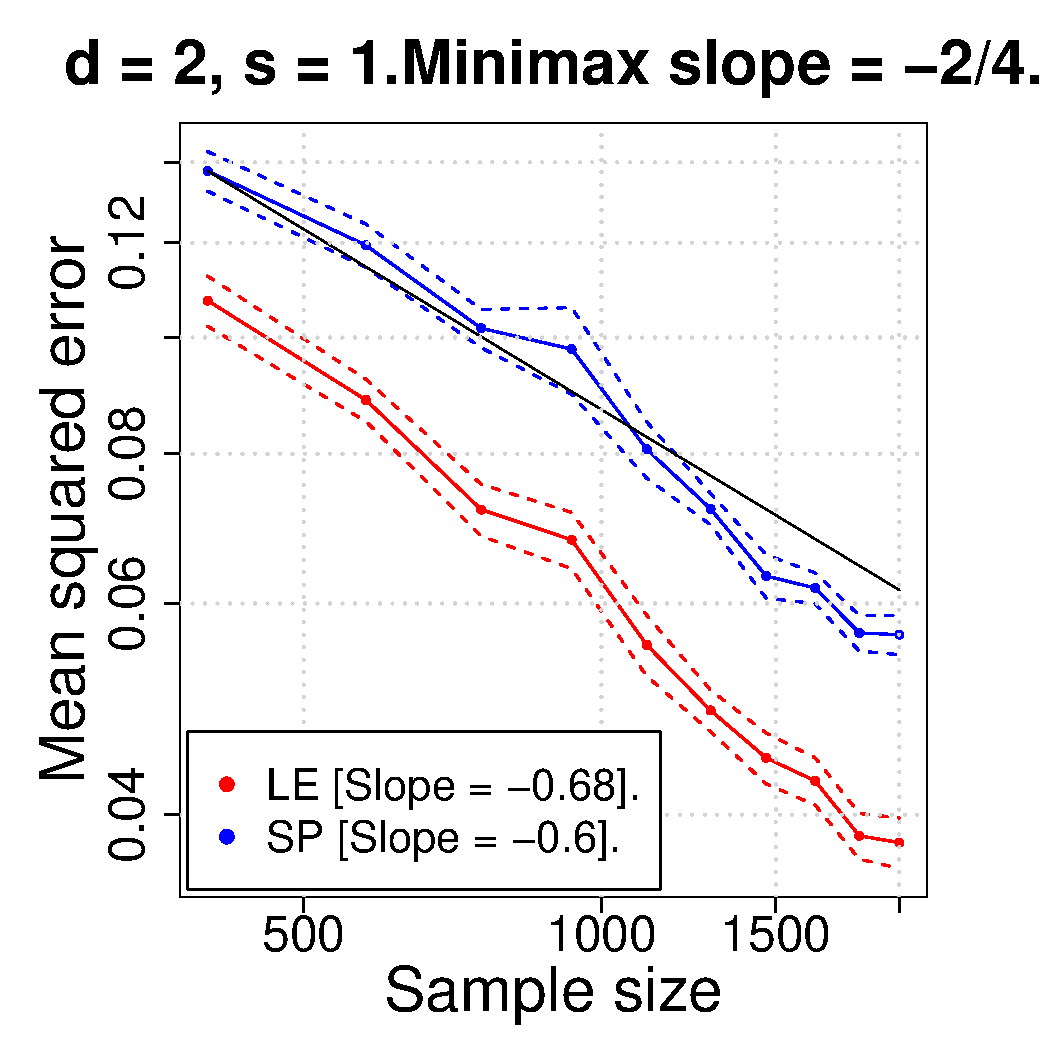
\includegraphics[width=.245\textwidth]{figures/mse_by_sample_size_2d.pdf}
	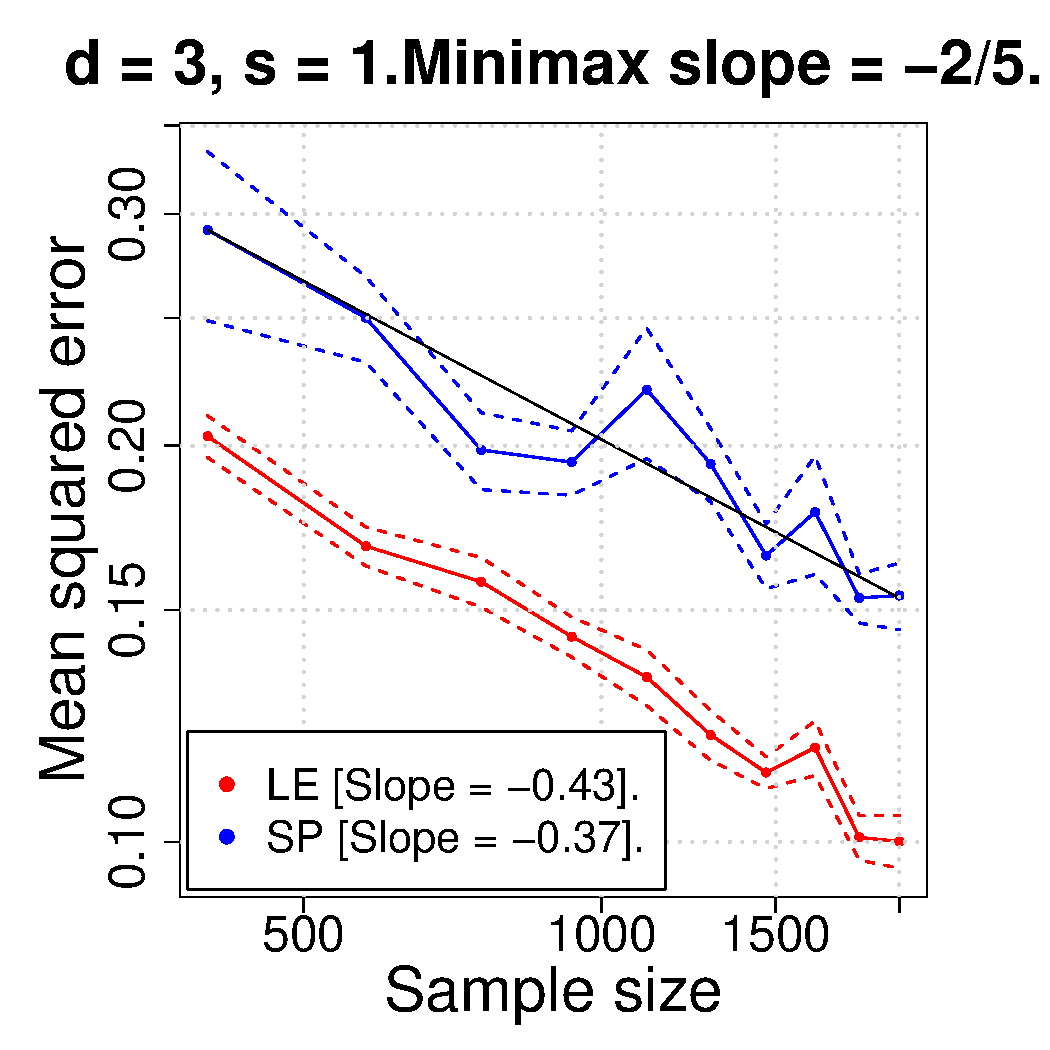
\includegraphics[width=.245\textwidth]{figures/mse_by_sample_size_3d.pdf} 
	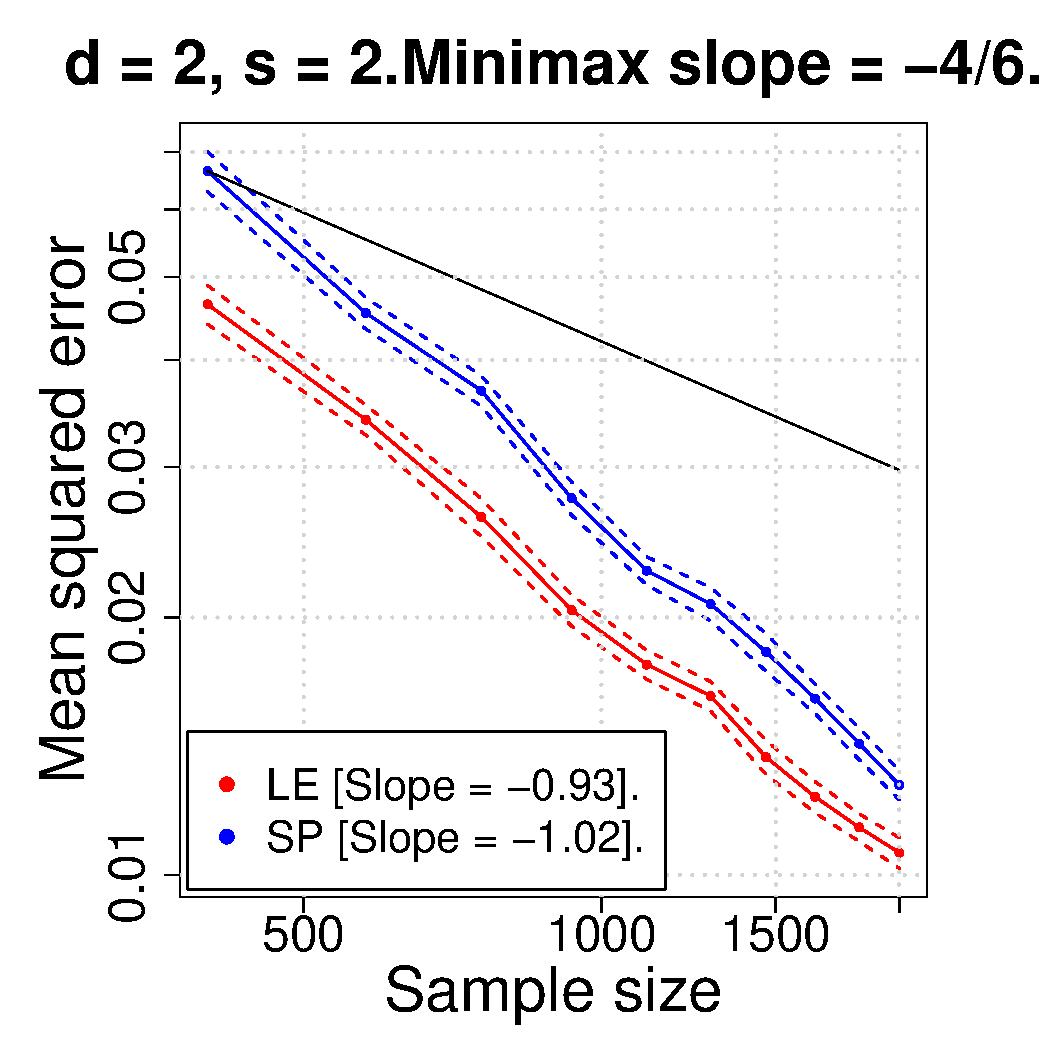
\includegraphics[width=.245\textwidth]{figures/mse_by_sample_size_2d_2s.pdf}
	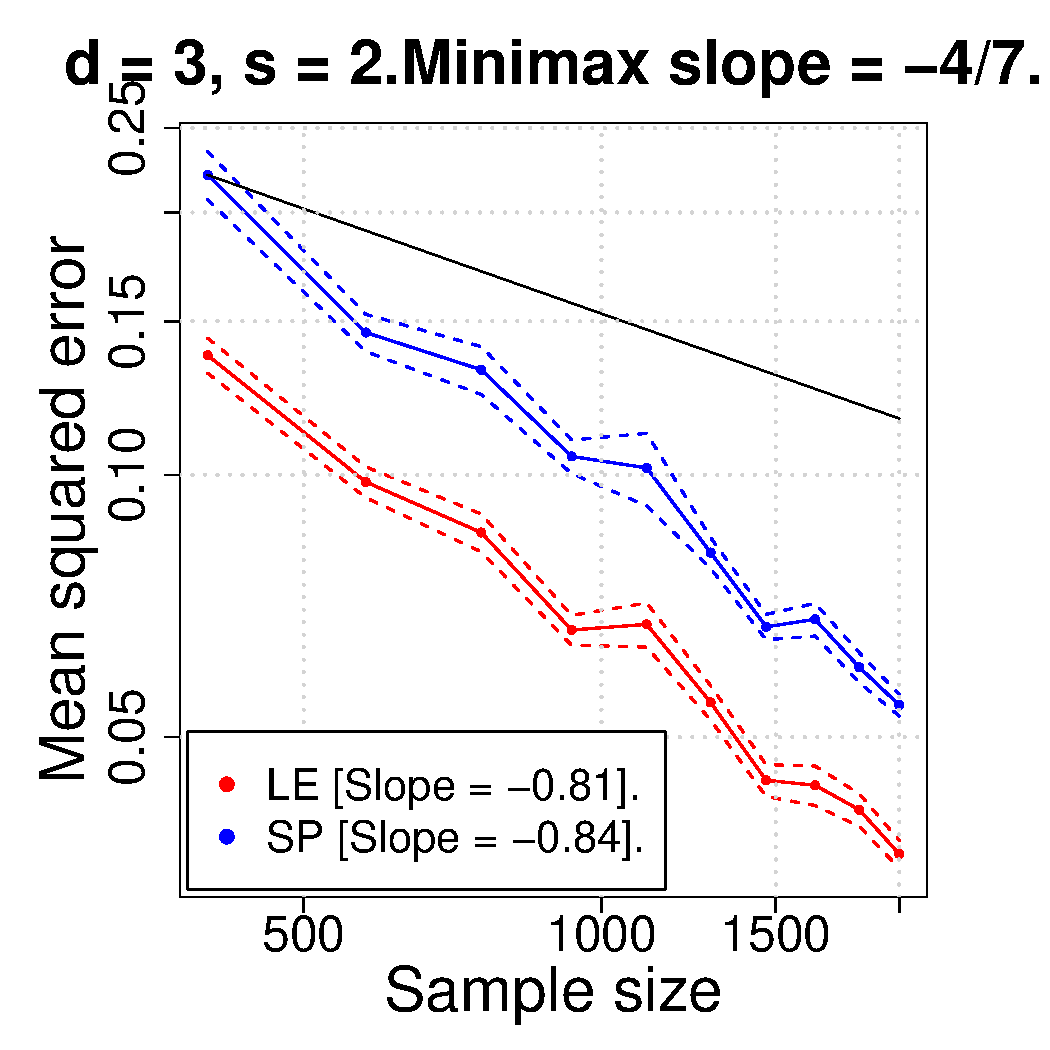
\includegraphics[width=.245\textwidth]{figures/mse_by_sample_size_3d_2s.pdf} 
	\caption{Mean squared error of Laplacian eigenmaps (\texttt{LE}) and a spectral projection estimator (\texttt{SP}) as a function of sample size $n$. Each plot is on the log-log scale, and the results are averaged over 50 repetitions. Both estimators are tuned for optimal average mean squared error. The black line shows the minimax rate (in slope only; the intercept is chosen to match the observed error).}
	\label{fig:fig1}
\end{figure*}

In Figure~\ref{fig:fig2} we compare tests using Laplacian eigenmaps and spectral projection. \textcolor{red}{(TODO): Need to ask Siva for help.}
\begin{figure*}[tb]
	\caption{Worst-case risk Laplacian eigenmaps (\texttt{LE}) and spectral projection (\texttt{SP}) tests, as a function of sample size $n$.}
	\label{fig:fig2}
\end{figure*}

These experiments demonstrate that in terms of statistical error, Laplacian eigenmaps methods are reasonable replacements for spectral projection methods. Laplacian eigenmaps depends on two tuning parameters, and in our final experiment we investigate the importance of both, focusing now on estimation. In Figure~\ref{fig:fig3}, we see how the mean-squared error of Laplacian eigenmaps changes as each tuning parameter is varied. As suggested by our theory, properly choosing the number of eigenvectors $K$ is crucial: the mse curves have a sharply defined minimum. On the other hand, as a function of the graph radius parameter $\varepsilon$ the mse curves are much closer to flat. This is particularly true in the first-order ($s = 1$) case, and still true albeit to a lesser extent when $s = 2$.   These findings reinforce two points we've made previously: first that Laplacian Eigenmaps should be viewed as a type of spectral projection method, in which the more important parameter to carefully tune is the number of eigenvectors $K$; second that the more regularity displayed by the regression function, the more important tuning the graph radius $\varepsilon$ becomes.

\begin{figure*}[tb]
	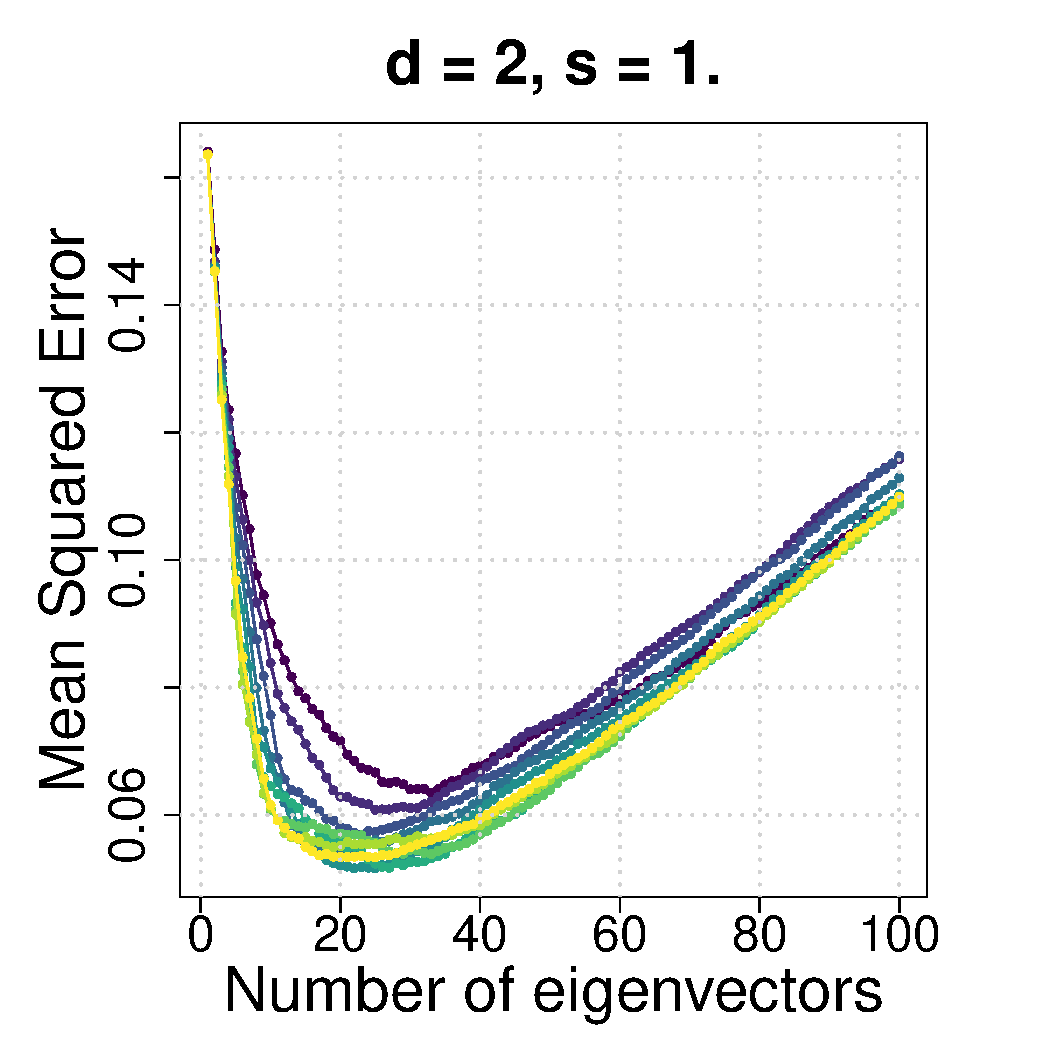
\includegraphics[width=.245\textwidth]{figures/eigenmaps_parameters/mse_by_number_of_eigenvectors.pdf}
	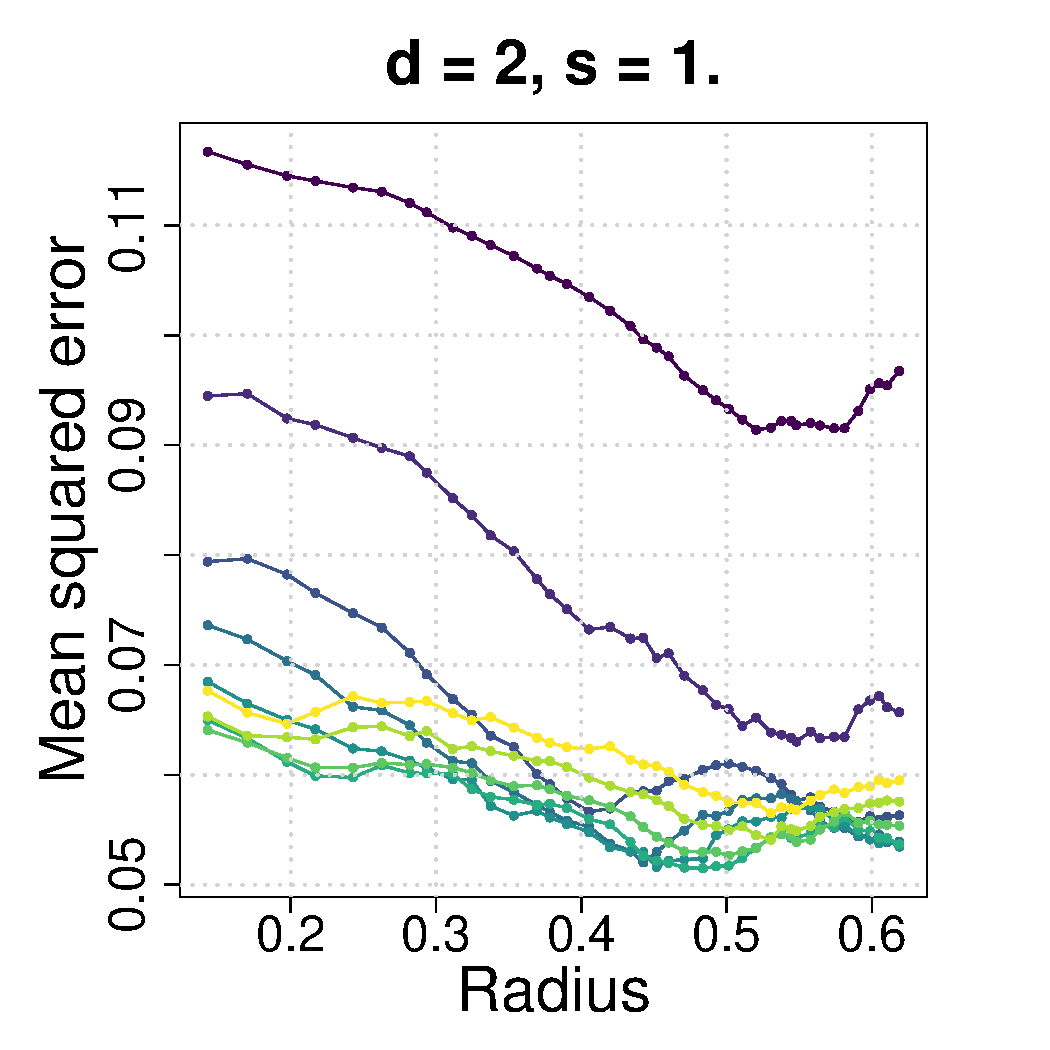
\includegraphics[width=.245\textwidth]{figures/eigenmaps_parameters/mse_by_radius.pdf} 
	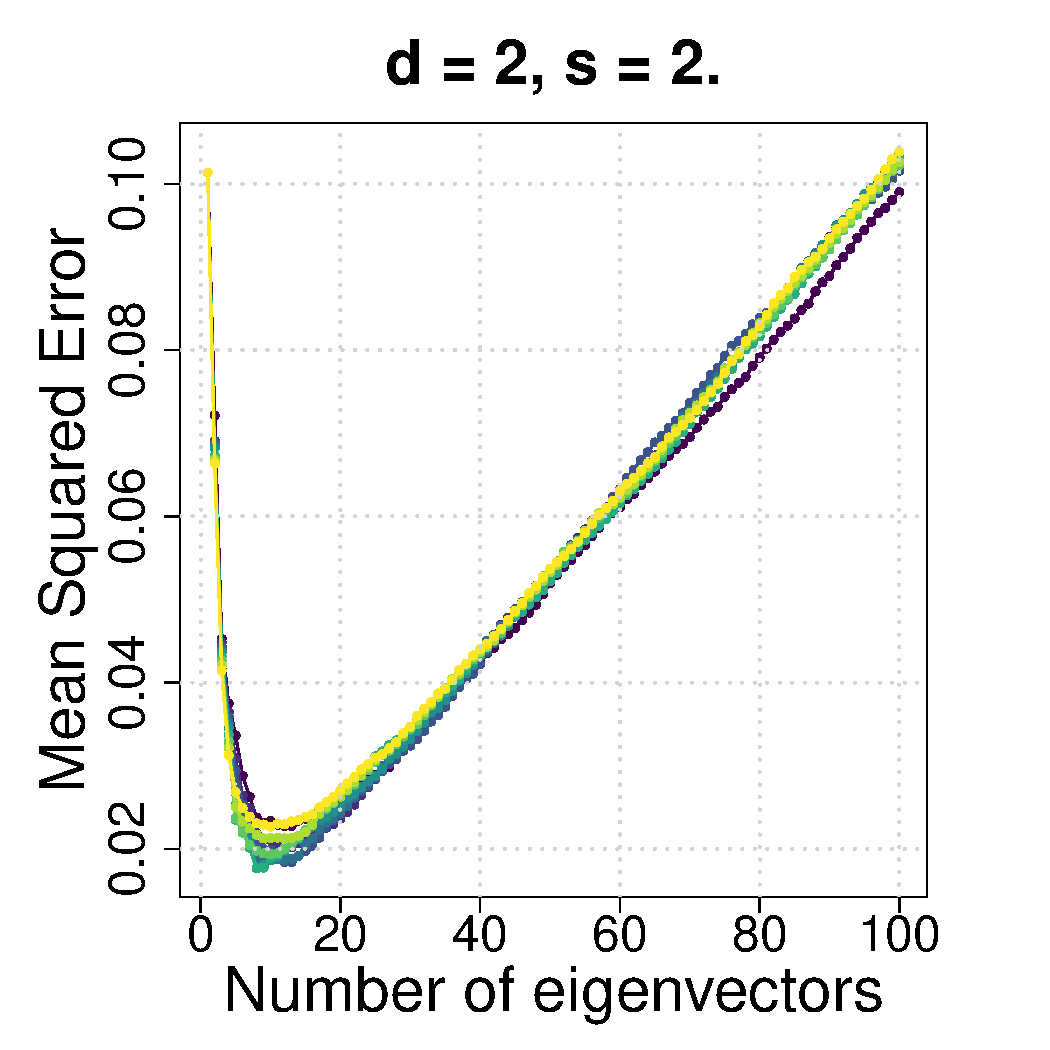
\includegraphics[width=.245\textwidth]{figures/eigenmaps_parameters_2s/mse_by_number_of_eigenvectors.pdf}
	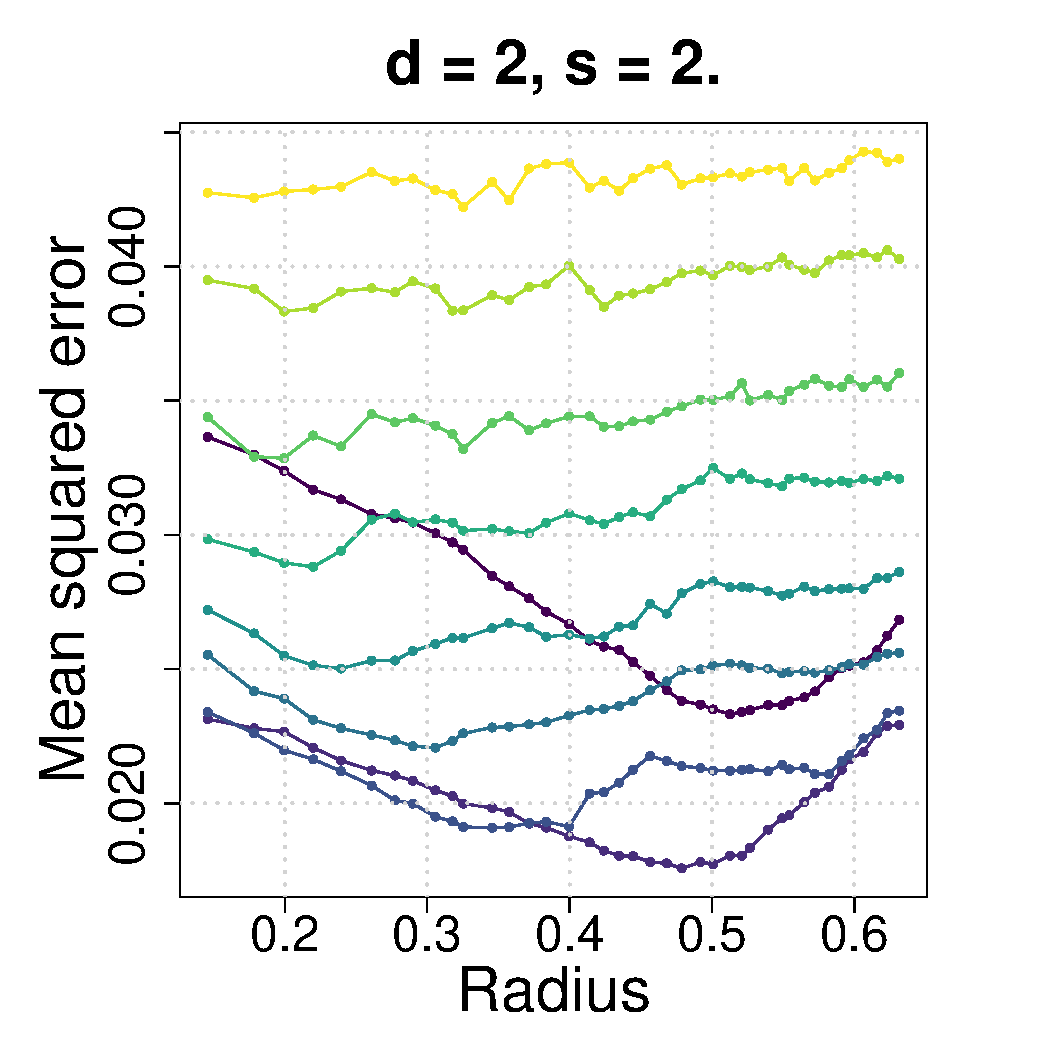
\includegraphics[width=.245\textwidth]{figures/eigenmaps_parameters_2s/mse_by_radius.pdf} 
	\caption{Mean squared error of Laplacian Eigenmaps as a function of hyperparameters. For all experiments, sample size $n = 2000$, and the results are averaged over $50$ repetitions. Colors show~\textcolor{red}{(?)}}
	\label{fig:fig3}
\end{figure*}

\section{Discussion}
\label{sec:discussion}

\subsection{Comparison with other estimators}
In this paper, we have motivated Laplacian eigenmaps by viewing it as a noisy approximation of a classical spectral projection method, which is its most obvious counterpart. We have shown that Laplacian eigenmaps inherits the optimality properties of its more classical counterpart. We now discuss the relationship between Laplacian eigenmaps and three other approaches to nonparametric regression. The first two---nonparametric least squares and kernel smoothing---are classical, whereas the third---Laplacian smoothing---makes use of the graph Laplacian in a different way than Laplacian eigenmaps.

\paragraph{Nonparametric least squares.}
The standard recommended alternative to spectral projection methods, when the distribution $P$ is considered non-uniform or unknown, is to do least-squares. For example, suppose instead of knowing $\psi_1,\psi_2,\ldots$, we had access only to eigenfunctions $\phi_1,\phi_2,\ldots$ of an unweighted Laplace-Beltrami operator $\Delta$. Then letting $\Phi_K = \mathrm{span}\{\phi_1,\ldots,\phi_K\}$, the least-squares estimator and test statistic
\begin{equation*}
\wt{f}_{\mathrm{LS}} := \argmin_{f \in \Phi_K} \|Y - f\|_n^2,\textrm{and}~~\wt{T}_{\mathrm{LS}} = \|\wt{f}\|_{\nu}^2
\end{equation*}
are still rate-optimal over $H_0^s(\mc{X})$. This holds true for both Model~\ref{def:model_flat_euclidean} and~\ref{def:model_manifold}, and is a consequence of our assumption that $p$ is bounded away from $0$.

However, this is not a totally satisfactory fix. For one thing, the least squares approach just outlined requires that we know the domain $\mc{X}$, in the strong sense that we know the Laplace-Beltrami operator $\Delta$ defined on $\mc{X}$. Domain knowledge is generally precious information, and such strong knowledge of $\mc{X}$ seems particularly unrealistic in the case where $\mc{X}$ is a manifold, and $\Delta$ is the manifold Laplace-Beltrami operator. Additionally, even if we know $\mc{X}$, diagonalizing the Laplace-Beltrami operator $\Delta$ is quite difficult for all but a few special domains, such as the unit cube $\mc{X} = [0,1]^d$ or torus $\mc{X} = \mathbb{T}^d$.

\paragraph{Kernel smoothing.}
It is also natural to ask whether the two stage estimator $T_{h,n}\wh{f}$ defined in Section~\ref{sec:out_of_sample} has any advantage over the simpler approach of directly kernel smoothing the responses, i.e. using the estimator $T_{h,n}Y$ (possibly for a different choice of $h$). In Appendix~\ref{subsec:eigenmaps_beats_kernel_smoothing}, we answer this question in the affirmative, by giving a simple example of a sequence of densities and regression functions $\{(p^{(n)}, f_0^{(n)}: n \in \mathbb{N}\}$ such that $\Ebb\|f_0 - T_{h,n}\wh{f}\|_P^2$ is of a strictly lower order than $\inf_{h'} \Ebb\|f_0 - T_{h',n}Y\|_P^2$. This is possible because Laplacian eigenmaps induces a completely different bias than kernel smoothing. For example, when $f_0$ and $p$ satisfy the so-called \emph{cluster} assumption--- e.g. $f_0$ is piecewise constant in high-density regions (clusters) of $p$--- then the bias of Laplacian eigenmaps can much smaller than that of kernel smoothing (for equivalent levels of variance). 

We emphasize that this does not contradict the well-known fact that kernel smoothing is an optimal method for nonparametric regression over e.g. H\"{o}lder balls. It simply reflects that in the standard nonparametric regression setup---which we adopt in the main part of this paper, and in which $P$ is assumed to be equivalent to Lebesgue measure---the biases of Laplacian eigenmaps and kernel smoothing are equivalent. On the other hand, when $f_0$ and $p$ satisfy some special relationship, such as the cluster assumption, the biases of these two methods can be quite different. There has been some work \textcolor{red}{(Rigollet, Wasserman, Niyogi, El Alaoui)} analyzing semi-supervised learning under various instantiations of the cluster assumption. However, a comprehensive analysis of various methods, including Laplacian eigenmaps and kernel smoothing, in this setting remains outstanding.

\paragraph{Laplacian smoothing.}
As mentioned previously, graph Laplacian smoothing uses the graph Laplacian $L_{n,\varepsilon}$ to form the penalty in a penalized least squares estimator. It can be calculated by one solve of a sparse, diagonally dominant linear system. Thus it should be much faster to compute than Laplacian eigenmaps, in which one must find (many) eigenvectors of $L_{n,\varepsilon}$. On the other hand, Laplacian smoothing is known to be minimax rate-optimal only in very limited regimes (over the Sobolev spaces $H^1(\mc{X})$ for $1 \leq d < 4$.) In contrast, we have shown that Laplacian eigenmaps is minimax rate-optimal for all $d$ (when $s = 1$) . We have also shown that Laplacian eigenmaps can adapt to higher-order smoothness, i.e. it can be minimax rate-optimal when $s > 1$. Thus, the known statistical properties of Laplacian eigenmaps are much stronger than those of Laplacian smoothing. 

\subsection{Future Work}
We view our work can be viewed as a contribution both to the fields of nonparametric regression with series estimators, and to graph-based learning. We end our discussion by mentioning some open work in each of these directions. 

Much is known about classical spectral projection methods beyond their rate optimality. For instance: such estimators and tests exhibit \emph{sharp optimality}, meaning their risk is within a $(1 + o(1))$ factor of the optimal risk; they can adapt to unknown smoothness of the regression function; they can be used to estimate smooth functionals of the regression function;  finally, they can be used to form confidence sets in $L^2(P)$. It would be interesting to see if Laplacian eigenmaps could replicate the performance of classical methods in any, or all, of these problems.

On the other hand, there are many variants of Laplacian eigenmaps worth considering. For instance, one can change the graph under consideration (e.g. by using the k-nearest neighbors), or the normalization of the graph Laplacian $L_{n,\varepsilon}$ (e.g. by using the symmetric normalized Laplacian). The former is practically useful, because it typically leads to connected graphs while always ensuring a given level of edge sparsity. In the latter, the graph Laplacian converges to a different limiting operator, which possesses different eigenvectors than $\Delta_P$ and thereby induces a different bias. We believe that under the setup we consider here, both methods will continue to be optimal.


\bibliographystyle{plainnat}
\bibliography{../../graph_regression_bibliography} 

\appendix

\noindent 

\section{Graph-dependent error bounds}
\label{sec:fixed_graph_error_bounds}
In this section, we adopt the fixed design perspective; or equivalently, condition on $X_i = x_i$ for $i = 1,\ldots,n$. Let $G = \bigl([n],W\bigr)$ be a fixed graph on $\{1,\ldots,n\}$ with Laplacian matrix $L = \sum_{k = 1}^{n}\lambda_k v_k v_k^{\top}$; the eigenvectors have unit empirical norm, $\|v_k\|_n^2 = 1$. The randomness thus all comes from the responses 
\begin{equation}
\label{eqn:fixed_graph_regression_model}
Y_i = f_{0}(x_i) + w_i
\end{equation}
where the noise variables $w_i$ are independent $N(0,1)$. In the rest of this section, we will mildly abuse notation and write $f_0 = (f_0(x_1),\ldots,f_0(x_n)) \in \Reals^n$. We will also write ${\bf Y} = (Y_1,\ldots,Y_n)$.

\subsection{Upper bound on Estimation Error of Laplacian Eigenmaps}

\begin{lemma}
	\label{lem:fixed_graph_estimation}
	For any integer $s > 0$, and any integer $0 \leq K \leq n$, the Laplacian eigenmaps estimator $\wh{f}$ of~\eqref{eqn:laplacian_eigenmaps_estimator} satisfies
	\begin{equation}
	\label{eqn:fixed_graph_estimation}
	\|\wh{f} - f_0\|_n^2 \leq \frac{\dotp{L^sf_0}{f_0}_n}{\lambda_{K + 1}^s} + \frac{5K}{n};
	\end{equation}
	this is guaranteed if $K = 0$, and otherwise holds with probability at least $1 - \exp(-K)$ if $1 \leq K \leq n$. 
\end{lemma}
\paragraph{Proof (of Lemma~\ref{lem:fixed_graph_estimation}).}
	By the triangle inequality,
	\begin{equation}
	\label{pf:fixed_graph_estimation_1}
	\|\wh{f} - f_0\|_n^2 \leq 2\Bigl(\|\mathbb{E}\wh{f} - f_0\|_n^2 + \|\wh{f} - \mathbb{E}\wh{f}\|_n^2\Bigr).
	\end{equation}
	The first term in~\eqref{pf:fixed_graph_estimation_1} (approximation error) is non-random, since the design is fixed. The expectation $\mathbb{E}\wh{f} = \sum_{k = 1}^{K} \dotp{v_k}{f_0}_n v_k$, so that
	\begin{equation*}
	\|\mathbb{E}\wh{f} - f_0\|_n^2 = \Bigl\|\sum_{k = K + 1}^{n} \dotp{v_k}{f_0}_n v_k\Bigr\|_n^2 = \sum_{k = K + 1}^n \dotp{v_k}{f_0}_n^2.
	\end{equation*}
	In the above, the last equality relies on the fact that $v_k$ are orthonormal in $L^2(P_n)$. Using the fact that the eigenvalues are in increasing order, we obtain
	\begin{equation*}
	\sum_{k = K + 1}^n \dotp{v_k}{f_0}_n^2 \leq \frac{1}{\lambda_{K + 1}^s} \sum_{k = K + 1}^n \lambda_k^s \dotp{v_k}{f_0}_n^2 \leq \frac{\dotp{L^sf_0}{f_0}_n}{\lambda_{K + 1}^s}.
	\end{equation*}
	
	If $K = 0$, $\wh{f} = \Ebb{\wh{f}} = 0$, and the second term in~\eqref{pf:fixed_graph_estimation_1} is $0$. Otherwise the second   in~\eqref{pf:fixed_graph_estimation_1} (estimation error) is random. Observe that $\dotp{v_k}{\varepsilon}_n \overset{d}{=} Z_k/\sqrt{n}$, where $(Z_1,\ldots,Z_n) \sim N(0,I_{n \times n})$. Again using the orthonormality of the eigenvectors $v_k$, we have
	\begin{equation*}
	\|\wh{f} - \mathbb{E}\wh{f}\|_n^2 = \sum_{k = 1}^{K} \dotp{v_k}{\varepsilon}_n^2 \overset{d}{=} \frac{1}{n}\sum_{k = 1}^{K} Z_k^2.
	\end{equation*}
	Thus $\|\wh{f} - \mathbb{E}\wh{f}\|_n^2$ is equal to $1/n$ times a $\chi^2$ distribution with $K$ degrees of freedom. Consequently, it follows from a result of \citep{laurent00} that
	\begin{equation*}
	\Pbb\biggl(\|\wh{f} - \mathbb{E}\wh{f}\|_n^2 \geq \frac{K}{n} + 2\frac{\sqrt{K}}{n}\sqrt{t} + \frac{2t}{n}\biggr) \leq \exp(-t).
	\end{equation*}
	Setting $t = K$ completes the proof of the lemma.

\subsection{Upper bound on Testing Error of Laplacian Eigenmaps}

Let $\wh{T} = \sum_{k = 1}^{K} \dotp{{\bf Y}}{v_k}_n^2$, and let $\varphi = \1\{\wh{T} \geq t_a\}$. In the following Lemma, we upper bound the Type I and Type II error of the test $\varphi$.

\begin{lemma}
	\label{lem:fixed_graph_testing}
	Suppose we observe $(Y_1,x_1),\ldots,(Y_n,x_n)$ according to~\eqref{eqn:fixed_graph_regression_model}.
	\begin{itemize}
		\item If $f_0 = 0$, then $\Ebb_0[\varphi] \leq a$.
		\item Suppose $f_0 \neq 0$ satisfies
		\begin{equation}
		\label{eqn:fixed_graph_testing_critical_radius}
		\|f_0\|_n^2 \geq \frac{\dotp{L^sf_0}{f_0}_n}{\lambda_{K + 1}^s} + \frac{\sqrt{2K}}{n}\biggl[2\sqrt{\frac{1}{a}} + \sqrt{\frac{2}{b}} + \frac{32}{bn}\biggr],
		\end{equation}
		for some $s \in \mathbb{N}\setminus \{0\}$. Then $\Ebb_{f_0}[1 - \phi] \leq b$.
	\end{itemize}
\end{lemma}
\paragraph{Proof (of Lemma~\ref{lem:fixed_graph_testing}).}
We first compute the expectation and variance of $\wh{T}$, then apply Chebyshev's inequality to upper bound the Type I and Type II error.

\underline{\emph{Expectation}.}
Recall that $\wh{T} = \sum_{k = 1}^{K} \dotp{Y}{v_k}_n^2$. Expanding the square gives
\begin{equation*}
\Ebb[\wh{T}] = \sum_{k = 1}^{K} \Ebb[\dotp{Y}{v_k}_n^2] = \sum_{k = 1}^{K} \dotp{f_0}{v_k}_n^2 + \Ebb[2\dotp{f_0}{v_k}_n\dotp{\varepsilon}{v_k}_n + \dotp{\varepsilon}{v_k}_n^2] = \frac{K}{n} + \sum_{k = 1}^{K} \dotp{f_0}{v_k}_n^2.
\end{equation*}
Thus $\Ebb[\wh{T}] - t_a = \sum_{k = 1}^{K} \dotp{f_0}{v_k}_n^2 - \sqrt{2K}/n \cdot \sqrt{1/a}$. Furthermore, it is a consequence of~\eqref{eqn:fixed_graph_testing_critical_radius} that 
\begin{equation}
\label{pf:fixed_graph_testing_1}
\sum_{k = 1}^{K} \dotp{f_0}{v_k}_n^2 - \frac{\sqrt{2K}}{n}\sqrt{1/a} \geq \|f_0\|_n^2 - \frac{\dotp{L^sf_0}{f_0}_n}{\lambda_{K + 1}^s} - \frac{\sqrt{2K}}{n}\sqrt{1/a} \geq \frac{\sqrt{2K}}{n}\biggl[\sqrt{\frac{1}{a}} + \sqrt{\frac{2}{b}} + \frac{32}{bn}\biggr].
\end{equation} 

\underline{\emph{Variance}.}
Recall from the proof of Lemma~\ref{lem:fixed_graph_estimation} that $\dotp{\varepsilon}{v_k}_n \overset{d}{=} Z_k/\sqrt{n}$ for $(Z_1,\ldots,Z_n) \sim N(0,I_{n \times n})$. Expanding the square, and recalling that $\Cov[Z,Z^2] = 0$ for Gaussian random variables, we have that
\begin{equation*}
\Var\bigl[\dotp{{\bf Y}}{v_k}_n^2\bigr] = \Var\biggl[\frac{2}{n}\dotp{f_0}{v_k}_nZ_k + \frac{2}{n^2}Z_k^2\biggr] = \frac{4\dotp{f_0}{v_k}_n^2}{n} + \frac{2}{n^2}.
\end{equation*}
Moreover, since $\Cov[Z_k^2,Z_{\ell}^2] = 0$ for each $k = 1,\ldots,K$, we see that
\begin{equation*}
\Var\bigl[\wh{T}\bigr] = \sum_{k = 1}^{K} \Var\bigl[\dotp{{\bf Y}}{v_k}_n^2\bigr] = \frac{2K}{n^2} + \sum_{k = 1}^{K}\frac{4\dotp{f_0}{v_k}_n^2}{n}.
\end{equation*}

\underline{\emph{Bounds on Type I and Type II error}.}
The upper bound on Type I error follows immediately from Chebyshev's inequality. 

The upper bound on Type II error also follows from Chebyshev's inequality. We observe that~\eqref{eqn:fixed_graph_testing_critical_radius} implies $\Ebb_{f_0}[\wh{T}] = t_a$, and apply Chebyshev's inequality to deduce
\begin{equation*}
\Pbb_{f_0}\bigl(\wh{T} < t_a\bigr) \leq \Pbb_{f_0}\Bigl(|\wh{T} - \Ebb_{f_0}[\wh{T}]|^2 > |\Ebb_{f_0}[\wh{T}] - t_a|^2\Bigr) \leq \frac{\Var\bigl[\wh{T}\bigr]}{\bigl[\Ebb_{f_0}[\wh{T}] - t_a\bigr]^2} = \frac{2K/n^2 + 4/n\sum_{k = 1}^{K}\dotp{f_0}{v_k}_n^2}{\bigl[\Ebb_{f_0}[\wh{T}] - t_a\bigr]^2}.
\end{equation*}
Thus we have upper bounded the Type II error by the sum of two terms, each of which are no more than $1/(2b)$, as we now show. For the first term, after noting that~\eqref{pf:fixed_graph_testing_1} implies $\Ebb_{f_0}[\wh{T}] - t_a \geq \sqrt{2K}/n \cdot \sqrt{2/b}$, the upper bound follows:
\begin{equation*}
\frac{2K/n^2}{\bigl[\Ebb_{f_0}[\wh{T}] - t_a\bigr]^2} \leq \frac{b}{2}.
\end{equation*}
On the other hand, for the second term we use~\eqref{pf:fixed_graph_testing_1} in two ways: first to conclude that $\Ebb_{f_0}[\wh{T}] - t_a \geq 1/2 \cdot \sum_{k = 1}^{K}\dotp{f_0}{v_k}_n^2$, and second to obtain
\begin{equation*}
\frac{4\sum_{k = 1}^{K}\dotp{f_0}{v_k}_n^2}{n\bigl[\Ebb_{f_0}[\wh{T}] - t_a\bigr]^2} \leq \frac{4\sum_{k = 1}^{K}\dotp{f_0}{v_k}_n^2}{n\bigl(\sum_{k = 1}^{K}\dotp{f_0}{v_k}_n^2/2\bigr)^2} \leq \frac{16}{n\sum_{k = 1}^{K}\dotp{f_0}{v_k}_n^2} \leq \frac{b}{2}.
\end{equation*}

\section{Graph Sobolev semi-norm, flat Euclidean domain}
\label{sec:graph_quadratic_form_euclidean}
In this section we prove Proposition~\ref{prop:graph_seminorm_ho}. The proposition will follow from several intermediate results.
\begin{enumerate}
	\item~In Section~\ref{subsec:decomposition_graph_seminorm}, we show that
	\begin{equation}
	\label{pf:graph_seminorm_ho_1}
	\dotp{L_{n,\varepsilon}^sf}{f}_n \leq \frac{1}{\delta} \dotp{L_{P,\varepsilon}^sf}{f}_{P} + \frac{C\varepsilon^2}{\delta n\varepsilon^{2 + d}}M^2.
	\end{equation}
	with probability at least $1 - 2\delta$. 
	
	We term the first term on the right hand side the \emph{non-local Sobolev semi-norm}, as it is a kernelized approximation to the Sobolev semi-norm $\dotp{\Delta_P^sf}{f}_{P}$. The second term on the right hand side is a pure bias term, which as we will see is negligible compared to the non-local Sobolev semi-norm as long as $\varepsilon \ll n^{-1/(2(s -1 + d))}$. 
	\item~In Section~\ref{subsec:approximation_error_nonlocal_laplacian}, we show that when $x$ is sufficiently in the interior of $\mc{X}$, then $L_{P,\varepsilon}^kf(x)$ is a good approximation to $\Delta_P^kf(x)$, as long as $f \in H^{s}(\mc{X})$ and $p \in C^{s - 1}(\mc{X})$ for some $s \geq 2k + 1$. 
	\item~In Section~\ref{subsec:boundary_behavior_nonlocal_laplacian}, we show that when $x$ is sufficiently near the boundary of $\mc{X}$, then $L_{P,\varepsilon}^kf(x)$ is close to $0$, as long as $f \in H_0^{s}(\mc{X})$ for some $s > 2k$.
	\item~In Section~\ref{subsec:estimate_nonlocal_seminorm}, we use the results of the preceding two sections to show that if $f \in H_0^s(\mc{X};M)$ and $p \in C^{s - 1}(\mc{X})$, there exists a constant $C$ which does not depend on $f$ such that
	\begin{equation}
	\label{pf:graph_seminorm_ho_2}
	\dotp{L_{P,\varepsilon}^sf}{f}_{P} \leq CM^2.
	\end{equation}
\end{enumerate}
Finally, in Section~\ref{subsec:integrals} we provide some assorted estimates used in Sections~\ref{subsec:decomposition_graph_seminorm}. 

\paragraph{Proof (of Proposition~\ref{prop:graph_seminorm_ho}).}
Proposition~\ref{prop:graph_seminorm_ho} follows immediately from~\eqref{pf:graph_seminorm_ho_1} and~\eqref{pf:graph_seminorm_ho_2}. \qed

One note regarding notation: suppose a function $g \in H^{\ell}(U)$, where $\ell \in \mathbb{N}$ and $U$ is an open set. Let $V$ be another open set, compactly contained within $U$. Then we will use the notation $g \in H^{\ell}(V)$ to mean that the restriction $\restr{g}{V}$ of $g$ to $V$ belongs to $H^{\ell}(V)$.

\subsection{Decomposition of graph Sobolev semi-norm}
\label{subsec:decomposition_graph_seminorm}

In Lemma~\ref{lem:graph_seminorm_bias}, we decompose the graph Sobolev semi-norm (a V-statistic) into an unbiased estimate of the non-local Sobolev semi-norm (a U-statistic), and a pure bias term. We establish that the pure bias term will be small (in expectation) relative to the U-statistic whenever $\varepsilon$ is sufficiently small.
\begin{lemma}
	\label{lem:graph_seminorm_bias}
	For any $f \in L^2(\mc{X})$, the graph Sobolev semi-norm satisfies
	\begin{equation}
	\label{eqn:graph_seminorm_bias_1}
	\dotp{L_{n,\varepsilon}^sf}{f}_{n} = U_{n,\varepsilon}^{(s)}(f) + B_{n,\varepsilon}^{(s)}(f),
	\end{equation}
	such that $\mathbb{E}[U_{n,\varepsilon}^{(s)}(f)] = (n - s - 1)!/n! \cdot \dotp{L_{P,\varepsilon}^sf}{f}_P$. If additionally $f \in H^1(\mc{X};M)$ and $\varepsilon \geq n^{-1/d}$, then the bias term $B_{n,\varepsilon}^{(s)}(f)$ satisfies
	\begin{equation}
	\label{eqn:graph_seminorm_bias_2}
	\mathbb{E}\bigl[|B_{n,\varepsilon}^{(s)}(f)|\bigr] \leq \frac{C\varepsilon^2}{\delta n\varepsilon^{2 + d}}M^2.
	\end{equation}
\end{lemma}
Then~\ref{pf:graph_seminorm_ho_1} follows immediately from Lemma~\ref{lem:graph_seminorm_bias}, by Markov's inequality.
\paragraph{Proof (of Lemma~\ref{lem:graph_seminorm_bias}).}
We begin by introducing some notation. We will use bold notation $\bj = (j_1,\ldots,j_s)$ for a vector of indices where $j_i \in [n]$ for each $i$. We write $[n]^s$ for the collection of all such vectors, and $(n)^s$ for the subset of such vectors with no repeated indices. Finally, we write $D_if$ for a kernelized difference operator,
\begin{equation*}
D_if(x) := \bigl(f(x) - f(X_i)\bigr) \eta\biggl(\frac{\|X_i - x\|}{\varepsilon}\biggr),
\end{equation*}
and we let $D_{\bj}f(x) := \bigl(D_{j_1}\circ \cdots \circ D_{j_s}f\bigr)(x)$.

With this notation in hand, it is easy to represent $\dotp{L_{n,\varepsilon}^sf}{f}_{n}$ as the sum of a U-statistic and a bias term,
\begin{align*}
\dotp{L_{n,\varepsilon}^sf}{f}_{n} & = \frac{1}{n} \sum_{i = 1}^{n} L_{n,\varepsilon}^sf(X_i) \cdot f(X_i) \\
& = \underbrace{\frac{1}{n^{s + 1}\varepsilon^{s(d + 2)}} \sum_{{i\bf j} \in (n)^{s + 1}}D_{\bj}f(X_i) \cdot f(X_i)}_{=:U_{n,\varepsilon}^{(s)}(f)} + \underbrace{\frac{1}{n^{s + 1}\varepsilon^{s(d + 2)}} \sum_{\substack{i\bj \in \\ [n]^{s + 1}\setminus (n)^{s + 1}}} D_{\bj}f(X_i) \cdot f(X_i)}_{=:B_{n,\varepsilon}^{(s)}(f)}
\end{align*}
When the indices of $i\bj$ are all distinct, it follows straightforwardly from the law of iterated expectation that
\begin{equation*}
\mathbb{E}[ D_{\bj}f(X_i) \cdot f(X_i)] = \varepsilon^{s(d + 2)}\mathbb{E}[L_{P,\varepsilon}^sf(X_i) \cdot f(X_i)] = \dotp{L_{P,\varepsilon}^sf}{f}_{P}, 
\end{equation*}
which in turn implies $\mathbb{E}[U_{n,\varepsilon}^{(s)}(f)] = (n - s - 1)!/n! \cdot \dotp{L_{P,\varepsilon}^sf}{f}_P$. 

It remains to show~\eqref{eqn:graph_seminorm_bias_2}. By adding and subtracting $f(X_{\bj_1})$, we obtain by symmetry that
\begin{equation*}
\sum_{\substack{i\bj \in \\ [n]^{s + 1}\setminus (n)^{s + 1}}} D_{\bj}f(X_i) \cdot f(X_i) = \frac{1}{2} \cdot \sum_{\substack{i\bj \in \\ [n]^{s + 1}\setminus (n)^{s + 1}}} D_{\bj}f(X_i) \cdot \bigl(f(X_i) - f(X_{\bj_1})\bigr),
\end{equation*}
and consequently
\begin{equation*}
\Ebb\Bigl[\sum_{\substack{i\bj \in \\ [n]^{s + 1}\setminus (n)^{s + 1}}} D_{\bj}f(X_i) \cdot f(X_i)\Bigr] \leq \frac{1}{2} \cdot \sum_{\substack{i\bj \in \\ [n]^{s + 1}\setminus (n)^{s + 1}}} \Ebb\Bigl[\bigl|D_{\bj}f(X_i)\bigr| \cdot \bigl|f(X_i) - f(X_{\bj_1})\bigr|\Bigr].
\end{equation*}
In Lemma~\ref{lem:graph_seminorm_bias2}, we show that if $f \in H^1(\mc{X};M)$, then for any $i\bj \in [n]^{s + 1}$ which contains a total of $k + 1$ distinct indices, 
\begin{equation*}
\Ebb\Bigl[\bigl|D_{\bj}f(X_i)\bigr| \cdot \bigl|f(X_i) - f(X_{\bj_1})\bigr|\Bigr] \leq C_1 \varepsilon^{2 + kd} M^2.
\end{equation*}
This shows us that the expectation of $|B_{n,\varepsilon}^s(f)|$ can bounded from above by the sum over several different terms, as follows:
\begin{align*}
\Ebb\Bigl[|B_{n,\varepsilon}^s(f)|\Bigr] & \leq C_1\frac{\varepsilon^2}{n\varepsilon^{2s}}M^2 \sum_{\substack{i\bj \in \\ [n]^{s + 1}\setminus (n)^{s + 1}}} \frac{1}{(n\varepsilon^d)^s}  \varepsilon^{(|i\bj| - 1)d} \\
& \leq C_1\frac{\varepsilon^2}{n\varepsilon^{2s}}M^2  \sum_{k = 1}^{s - 1} \frac{(n\varepsilon^d)^k}{(n\varepsilon^d)^s}n.
\end{align*}
Finally, we note that by assumption $n\varepsilon^d \geq 1$, so that in the above sum the factor of $(n\varepsilon^d)^k$ is largest when $k = s- 1$. We conclude that
\begin{equation*}
\Ebb\Bigl[|B_{n,\varepsilon}^s(f)|\Bigr] \leq C_1 (s - 1) \frac{\varepsilon^2}{n\varepsilon^{2s + d}}M^2,
\end{equation*}
which is the desired result.

\subsection{Approximation error of non-local Laplacian}
\label{subsec:approximation_error_nonlocal_laplacian}

In this section, we establish the convergence $L_{P,\varepsilon}^kf \to \sigma_{\eta}^k\Delta_P^kf$ as $\varepsilon \to 0$. More precisely, we give an upper bound on the squared difference between $L_{P,\varepsilon}^kf$ and  $\sigma_{\eta}^k\Delta_P^kf$ as a function of $\varepsilon$. The bound holds for all $x \in \mc{X}_{k\varepsilon}$, and $f \in H^{s}(\mc{X})$, as long as $s \geq 2k + 1$.  \textcolor{red}{(TODO): Make sure that $\sigma_{\eta}$ is defined somewhere.}
\begin{lemma}
	\label{lem:approximation_error_nonlocal_laplacian}
	Assume Model~\ref{def:model_flat_euclidean}. Let $s \in \mathbb{N} \setminus \{0,1\}$, suppose that $f \in H^s(\mc{X};M)$, and if $s > 1$ suppose that $p \in C^{s - 1}(\mc{X})$. Let $L_{P,\varepsilon}$ be define with respect to a kernel $\eta$ that satisfies~\ref{asmp:kernel_flat_euclidean}. Then there exist constants $C_1$ and $C_2$ that do not depend on $f$, such that each of the following statements hold.
	\begin{itemize}
		\item If $s$ is odd and $k = (s - 1)/2$, then
		\begin{equation}
		\label{eqn:approximation_error_nonlocal_laplacian_1}
		\|L_{P,\varepsilon}^kf - \Delta_P^kf\|_{L^2(\mc{X}_{k\varepsilon})} \leq C_1 M \varepsilon
		\end{equation}
		\item If $s$ is even and $k = (s - 2)/2$, then
		\begin{equation}
		\label{eqn:approximation_error_nonlocal_laplacian_2}
		\|L_{P,\varepsilon}^kf - \Delta_P^kf\|_{L^2(\mc{X}_{k\varepsilon})} \leq C_2 M \varepsilon^2.
		\end{equation}
	\end{itemize}
\end{lemma}
We remark that when $k = 1$ and $f \in C^3(\mc{X})$ or $C^4(\mc{X})$, statements of this kind are well known \textcolor{red}{(references)}, and indeed stronger results---with $L^{\infty}(\mc{X})$ norm replacing $L^2(\mc{X})$ norm---hold. When dealing with the iterated Laplacian, and functions $f$ which are regular only in the Sobolev sense, the proof is somewhat more lengthy, but the spirit of the result is largely the same.
 
\paragraph{Proof (of Lemma~\ref{lem:approximation_error_nonlocal_laplacian}).}
Throughout this proof, we shall assume that $f$ and $p$ are smooth functions, meaning they belong to $C^{\infty}(\mc{X})$. This is without loss of generality, since $C^{\infty}(\mc{X})$ is dense in both $H^s(\mc{X})$ and $C^{s - 1}(\mc{X})$, and since both sides of the inequalities~\eqref{eqn:approximation_error_nonlocal_laplacian_1} and~\eqref{eqn:approximation_error_nonlocal_laplacian_2} are continuous with respect to $\|\cdot\|_{H^s(\mc{X})}$ and $\|\cdot\|_{C^{s - 1}(\mc{X})}$ norms.

We will actually prove a more general set of statements than contained in Lemma~\ref{lem:approximation_error_nonlocal_laplacian}, more general in the sense that they give estimates for all $k$, rather than simply the particular choices of $k$ given above. In particular, we will prove that the following two statements hold for any $s \in \mathbb{N}$ and any $k \in \mathbb{N} \setminus \{0\}$. 
\begin{itemize}
	\item If $k \geq s/2$, then for every $x \in \mc{X}_{k\varepsilon}$, 
	\begin{equation}
	\label{pf:approximation_error_nonlocal_laplacian_0}
	L_{P,\varepsilon}^kf(x) = g_s(x) \varepsilon^{s - 2k}
	\end{equation}
	for a function $g_s$ that satisfies
	\begin{equation}
	\label{pf:approximation_error_nonlocal_laplacian_0.5}
	\|g_s\|_{L^2(\mc{X}_{k\varepsilon})} \leq C \|p\|_{C^{q}(\mc{X})}^k M 
	\end{equation}
	where $q = 1$ if $s =0$ or $s = 1$, and otherwise $q = s - 1$. 
	\item If $k < s/2$, then for every $x \in \mc{X}_{k\varepsilon}$,
	\begin{equation}
	\label{pf:approximation_error_nonlocal_laplacian_1}
	L_{P,\varepsilon}^kf(x) = \sigma_{\eta}^k \cdot \Delta_{P}^kf(x) + \sum_{j = 1}^{\floor{(s - 1)/2} - k} g_{2(j + k)}(x)\varepsilon^{2j} + g_{s}(x) \varepsilon^{s - 2k}.
	\end{equation}
	for functions $g_j$ that satisfy
	\begin{equation}
	\label{pf:approximation_error_nonlocal_laplacian_1.5}
	\|g_j\|_{H^{s - j}(\mc{X}_{k\varepsilon})} \leq C \|p\|_{C^{s - 1}(\mc{X})}^k M.
	\end{equation}
\end{itemize}
In the statement above, recall that $H^0(\mc{X}_{k\varepsilon}) = L^2(\mc{X}_{k\varepsilon})$. Additionally, note that we may speak of the pointwise behavior of derivatives of $f$ because we have assumed that $f$ is a smooth function. Observe that~\eqref{eqn:approximation_error_nonlocal_laplacian_1} follows upon taking $k = \floor{(s - 1)/2}$ in~\eqref{pf:approximation_error_nonlocal_laplacian_1}, whence we have
\begin{equation*}
\bigl(L_{P,\varepsilon}^kf(x) - \sigma_{\eta}^k \Delta_{P}^kf(x)\bigr)^2 = \varepsilon^2 \bigl(g_s(x)\bigr)^2
\end{equation*}
for some $g_s \in \Leb^2(\mc{X}_{k\varepsilon},C \cdot M \cdot \|p\|_{C^{s - 1}(\mc{X})})$, and integrating over $\mc{X}_{k\varepsilon}$ gives the desired result. \eqref{eqn:approximation_error_nonlocal_laplacian_2} follows from~\eqref{pf:approximation_error_nonlocal_laplacian_1} in an identical fashion. 

It thus remains establish~\eqref{pf:approximation_error_nonlocal_laplacian_1}, and~\eqref{pf:approximation_error_nonlocal_laplacian_0} which is an important part of proving~\eqref{pf:approximation_error_nonlocal_laplacian_1}. We will do so by induction on $k$. Note that throughout, we will let $g_j$ refer to functions which may change from line to line, but which always satisfy~\eqref{pf:approximation_error_nonlocal_laplacian_1.5}. 

\underline{\textit{Proof of~\eqref{pf:approximation_error_nonlocal_laplacian_0} and~\eqref{pf:approximation_error_nonlocal_laplacian_1}, base case.}}

We begin with the base case, where $k = 1$. Again, we point out that although desired result is known when $s = 3$ or $s = 4$, and $f$ is regular in the H\"{o}lder sense, we require estimates for all $s \in \mathbb{N}$ when $f$ is regular in the Sobolev sense.

When $s = 0$, the inequality~\eqref{pf:approximation_error_nonlocal_laplacian_0} is implied by Lemma~\ref{lem:l2estimate_nonlocal_laplacian}.  When $s \geq 1$, we proceed using Taylor expansion. For any $x \in \mc{X}_{\varepsilon}$, we have that $B(x,\varepsilon) \subseteq \mc{X}$. Thus for any $x' \in B(x,\varepsilon)$, we may take an order $s$ Taylor expansion of $f$ around $x' = x$, and an order $q$ Taylor expansion of $p$ around $x' = x$, where $q = 1$ if $s = 1$, and otherwise $q = s - 1$. (See Section~\ref{subsec:taylor_expansion} for a review of the notation we use for Taylor expansions, as well as some properties that we make use of shortly.) This allows us to express $L_{P,\varepsilon}f(x)$ as the sum of three terms,
\begin{align*}
L_{P,\varepsilon}f(x) & = \frac{1}{\varepsilon^{d + 2}}\sum_{j_1 = 1}^{s - 1} \sum_{j_2 = 0}^{q - 1}\frac{1}{j_1!j_2!}  \int_{\mc{X}} \bigl(d_x^{j_1}f\bigr)(x' - x) \bigl(d_x^{j_2}p\bigr)(x' - x) \eta\biggl(\frac{\|x' - x\|}{\varepsilon}\biggr) \,dx' \quad + \\
& \quad \frac{1}{\varepsilon^{d + 2}}\sum_{j = 1}^{s - 1} \frac{1}{j!} \int_{\mc{X}} \bigl(d_x^jf\bigr)(x' - x)  r_{x'}^{q}(x;p) \eta\biggl(\frac{\|x' - x\|}{\varepsilon}\biggr) \,dx' \quad  + \\
& \quad \frac{1}{\varepsilon^{d + 2}} \int_{\mc{X}} r_{x'}^j(x;f) \eta\biggl(\frac{\|x' - x\|}{\varepsilon}\biggr) \,dP(x').
\end{align*}
Here we have adopted the convention that $\sum_{j = 1}^{0} = 0$. 

Changing variables to $z = (x' - x)/\varepsilon$, we can rewrite the above expression as 
\begin{align*}
L_{P,\varepsilon}f(x) & = \frac{1}{\varepsilon^{2}}\sum_{j_1 = 1}^{s - 1} \sum_{j_2 = 0}^{q - 1}\frac{\varepsilon^{j_1 + j_2}}{j_1!j_2!}  \int d_x^{j_1}f(z) d_x^{j_2}p(z) \eta\bigl(\|z\|\bigr) \,dz \quad + \\
& \quad \frac{1}{\varepsilon^{2}} \sum_{j = 1}^{s - 1} \frac{\varepsilon^j}{j!} \int d_x^jf(z)  r_{zh + x}^{q}(x;p) \eta\bigl(\|z\|\bigr) \,dz \quad  + \\
& \quad \frac{1}{\varepsilon^{2}} \int r_{zh + x}^j(x;f) \eta\bigl(\|z\|\bigr) p(zh + x)\,dz \\
& := G_1(x) + G_2(x) + G_3(x).
\end{align*}
We now separately consider each of $G_1(x),G_2(x)$ and $G_3(x)$. We will establish that if $s = 1$ or $s = 2$, then $G_1(x) = 0$, and otherwise if $s \geq 3$ that
\begin{equation*}
G_1(x) = \sigma_{\eta}\Delta_Pf(x) + \sum_{j = 1}^{\floor{(s - 1)/2} - 1}g_{2(j + 1)}(x)\varepsilon^{2j} + g_{s}(x)\varepsilon^{s - 2}.
\end{equation*}
On the other hand, we will establish that if $s = 1$ then $G_2(x) = 0$, and otherwise for $s \geq 2$
\begin{equation}
\label{pf:approximation_error_nonlocal_laplacian_2}
\|G_2\|_{\Leb^2(\mc{X}_{\varepsilon})} \leq C \varepsilon^{s - 2} M \|p\|_{C^{s - 1}(\mc{X})};
\end{equation}
this same estimate will hold for $G_3$ for all $s \geq 1$. Together these will imply~\eqref{pf:approximation_error_nonlocal_laplacian_0} and~\eqref{pf:approximation_error_nonlocal_laplacian_1}. 

\emph{Estimate on $G_1(x)$.}
If $s = 1$, then $s - 1 = 0$, and so $G_1(x) = 0$. We may therefore suppose $s \geq 2$. Recall that
\begin{equation}
G_1(x) = \sum_{j_1 = 1}^{s - 1} \sum_{j_2 = 0}^{q - 1} \frac{\varepsilon^{j_1 + j_2 - 2}}{j_1!j_2!}  \underbrace{\int_{B(0,1)} d_x^{j_1}f(z) d_x^{j_2}p(z) \eta(\|z\|) \,dz}_{:= g_{j_1,j_2}(x)} \label{pf:approximation_error_nonlocal_laplacian_3}
\end{equation}
The nature of $g_{j_1,j_2}(x)$ depends on the sum $j_1 + j_2$. Since $d_x^{j_1}f d_x^{j_2}$ is an order $j_1 + j_2$ (multivariate) monomial, we have (see Section~\ref{subsec:taylor_expansion}) that whenever $j_1 + j_2$ is odd,
\begin{equation*}
g_{j_1,j_2}(x) = \int_{\mc{X}} d_x^{j_1}f(z) d_x^{j_2}p(z) \eta(\|z\|) \,dz = 0.
\end{equation*}
In particular this is the case when $j_1 = 1$ and $j_2 = 0$. Thus when $s = 2$,  $G_1(x) = g_{1,0}(x) = 0$. On the other hand if $s \geq 3$, then the lowest order terms in~\eqref{pf:approximation_error_nonlocal_laplacian_3} are those where $j_1 + j_2 = 2$, so that either $j_1 = 1$ and $j_2 = 1$, or $j_1 = 2$ and $j_2 = 0$. We have that
\begin{align*}
g_{1,1}(x) + \frac{1}{2}g_{2,0}(x) & = \int_{\mc{X}} d_x^{1}f(z) d_x^{1}p(z) \eta(\|z\|) \,dz + \frac{p(x)}{2} \int_{\mc{X}} d_x^{2}f(z) \eta(\|z\|) \,dz \\
& = \sum_{i_1 = 1}^{d} \sum_{i_2 = 1}^{d} D^{e_{i_1}}f(x) D^{e_{i_2}}p(x) \int_{\mc{X}} z^{e_{i_1} + e_{i_2}} \eta(\|z\|) \,dz + \frac{p(x)}{2} \sum_{i_1 = 1}^{d} \sum_{i_2 = 1}^{d}D^{e_{i_2}+e_{i_2}}f(x)\int_{\mc{X}} z^{e_{i_1} + e_{i_2}} \eta(\|z\|) \,dz\\
& = \sum_{i = 1}^{d} D^{e_{i}}f(x) D^{e_{i}}p(x) \int_{\mc{X}} z^2 \eta(\|z\|) \,dz + \frac{p(x)}{2} \sum_{i = 1}^{d} D^{2e_{i}}f(x)\int_{\mc{X}} z^2 \eta(\|z\|) \,dz\\ 
& = \sigma_{\eta}\Delta_Pf(x),
\end{align*}
which is the leading term order term. Now it remains only to deal with the higher-order terms, where $j_1 + j_2 > 2$, and where it suffices to show that each function $g_{j_1,j_2}$ satisfies~\eqref{pf:approximation_error_nonlocal_laplacian_1.5} for $j = \min\{j_1 + j_2 - 2,s - 2\}$. It is helpful to write $g_{j_1,j_2}$ using multi-index notation, 
\begin{align*}
g_{j_1,j_2}(x) = \sum_{|\alpha_1| = j_1} \sum_{|\alpha_2| = j_2} D^{\alpha_1}f(x) D^{\alpha_2}p(x) \int_{B(0,1)} z^{\alpha_1 + \alpha_2} \eta(\|z\|) \,dz,
\end{align*}
where we note that $|\int_{B(0,1)} z^{\alpha_1 + \alpha_2} \eta(\|z\|) \,dz| < \infty$ for all $\alpha_1, \alpha_2$, by the assumption that $\eta$ is Lipschitz on its support. Finally, by H\"{o}lder's inequality we have that
\begin{align*}
\|D^{\alpha_1}f D^{\alpha_2}p\|_{H^{s - (j + 2)}(\mc{X})} & \leq \|D^{\alpha_1}f\|_{H^{s - (j + 2)}(\mc{X})} \|D^{\alpha_2}p\|_{C^{s - (j + 2)}(\mc{X})} \\
& \leq \|D^{\alpha_1}f\|_{H^{s - j_1}(\mc{X})} \|D^{\alpha_2}p\|_{C^{s - (j_2 + 1)}(\mc{X})} \\
& \leq M \cdot \|p\|_{C^{s - 1}(\mc{X})},
\end{align*}
and summing over all $|\alpha_1| = j_1$ and $|\alpha_2| = j_2$ establishes that $g_{j_1,j_2}$ satisfies~\eqref{pf:approximation_error_nonlocal_laplacian_1.5}.

\emph{Estimate on $G_2(x)$.}
Note immediately that $G_2(x) = 0$ if $s = 1$. Otherwise if $s \geq 2$, then $q = s - 1$. Recalling that $|r_{x + z\varepsilon}^{s - 1}(x; p)| \leq C\varepsilon^{s - 1}\|p\|_{C^{s - 1}(\mc{X})}$ for any $z \in B(0,1)$, and that $d_x^jf(\cdot)$ is a $j$-homogeneous function, we have that
\begin{align}
|G_2(x)| & \leq \sum_{j = 1}^{s - 1} \frac{\varepsilon^{j - 2}}{j!}\int_{B(0,1)} \Bigl|\bigl(d_x^{j}f\bigr)(z)\Bigr| \cdot |r_{x + z\varepsilon}^{s - 1}(x;p)| \cdot \eta(\|z\|) \,dz \nonumber \\
& \leq C\varepsilon^{s - 2}\|p\|_{C^{s - 1}(\mc{X})} \sum_{j = 1}^{s - 1} \frac{1}{j!} \int_{B(0,1)} \Bigl|\bigl(d_x^{j}f\bigr)(z)\Bigr| \cdot \eta(\|z\|) \,dz \label{pf:approximation_error_nonlocal_laplacian_4}.
\end{align}
Furthermore, for each $j = 1,\ldots,s - 1$ convolution of $d_x^jf$ with $\eta$ only decreases the $\Leb^2(\mc{X}_{\varepsilon})$ norm, meaning
\begin{equation}
\label{pf:approximation_error_nonlocal_laplacian_5}
\begin{aligned}
\int_{\mc{X}_{\varepsilon}} \biggl(\int_{B(0,1)} \Bigl|\bigl(d_x^{j}f\bigr)(z)\Bigr| \cdot \eta(\|z\|) \,dz\biggr)^2 \,dx & \leq \int_{\mc{X}_{\varepsilon}} \biggl(\int_{B(0,1)} \Bigl|\bigl(d_x^jf\bigr)(z)\Bigr|^2 \eta(\|z\|)\,dz \biggr) \cdot \biggl(\int_{B(0,1)} \eta(\|z\|) \,dz \biggr) \,dx \\
& \leq \int_{B(0,1)} \int_{\mc{X}_{\varepsilon}} \Bigl[\bigl(d^jf\bigr)(x)\Bigr]^2 \eta(\|z\|) \,dx  \,dz \\
& \leq \|d^jf\|_{\Leb^2(\mc{X_{\varepsilon}})}^2.
\end{aligned}
\end{equation}
In the above, we have used both that $|d_x^jf(z)| \leq |d^jf(x)|$ for all $z \in B(0,1)$, and that the kernel is normalized so that $\int \eta(\|z\|) \,dz = 1$. 
Combining this with~\eqref{pf:approximation_error_nonlocal_laplacian_4}, we conclude that
\begin{align*}
\int_{\mc{X}_{\varepsilon}} |G_2(x)|^2 \,dx & \leq C \Bigl(\varepsilon^{s - 2}\|p\|_{C^{s - 1}(\mc{X})}\Bigr)^2 \sum_{j = 1}^{s - 1} \int_{\mc{X}_{\varepsilon}}\biggl(\frac{1}{j!} \int_{B(0,1)} \Bigl|\bigl(d_x^{j}f\bigr)(z)\Bigr| \cdot \Bigl|\eta(\|z\|)\Bigr| \,dz\biggr)^2 \,dx \\
& \leq C \Bigl(\varepsilon^{s - 2}\|p\|_{C^{s - 1}(\mc{X})}\Bigr)^2 \sum_{j = 1}^{s - 1} \|d^ju\|_{\Leb^2(\mc{X_{\varepsilon}})}^2,
\end{align*}
establishing the desired estimate.

\emph{Estimate on $G_3(x)$.}
Applying the Cauchy-Schwarz inequality, we deduce a pointwise upper bound on $|G_3(x)|^2$,
\begin{align*}
|G_3(x)|^2 & \leq \biggl(\frac{p_{\max}}{\varepsilon^2}\biggr)^2 \cdot \biggl(\int_{B(0,1)} \bigl|r_{x + \varepsilon z}^s(x;u)\bigr|^2 \eta(\|z\|)\,dz\biggr) \cdot \biggl(\int_{B(0,1)} \eta(\|z\|) \,dz\biggr) \\
& \leq \biggl(\frac{p_{\max}}{\varepsilon^2}\biggr)^2 \int_{B(0,1)} \bigl|r_{x + \varepsilon z}^s(x;u)\bigr|^2 \eta(\|z\|) \,dz.
\end{align*}
Applying this pointwise over all $x \in \mc{X}_{\varepsilon}$ and integrating, we obtain
\begin{align*}
\int_{\mc{X}_{\varepsilon}} |G_3(x)|^2 \,dx & \leq \biggl(\frac{p_{\max}}{\varepsilon^2}\biggr)^2 \int_{\mc{X}_{\varepsilon}} \int_{B(0,1)} \bigl|r_{x + \varepsilon z}^s(x;f)\bigr|^2 \eta(\|z\|) \,dz \,dx \\
& = \biggl(\frac{p_{\max}}{\varepsilon^2}\biggr)^2 \int_{B(0,1)} \int_{\mc{X}_{\varepsilon}} \bigl|r_{x + \varepsilon z}^s(x;f)\bigr|^2 \eta(\|z\|) \,dx \,dz \\
& \leq \biggl(\frac{p_{\max}\varepsilon^s}{\varepsilon^2}\biggr)^2  \|d^sf\|_{L^2(\mc{X}_{\varepsilon})}^2,
\end{align*}
with the last inequality following from~\eqref{eqn:sobolev_remainder_term}. Noting that $p_{\max} = \|p\|_{C^0(\mc{X})} \leq \|p\|_{C^{s - 1}(\mc{X})}$, we see that this is a sufficient bound on $\|G_3\|_{\Leb^2(\mc{X}_{\varepsilon})}$.

\underline{\textit{Proof of~\eqref{pf:approximation_error_nonlocal_laplacian_0} and~\eqref{pf:approximation_error_nonlocal_laplacian_1}, induction step.}}
We now assume that~\eqref{pf:approximation_error_nonlocal_laplacian_0} and~\eqref{pf:approximation_error_nonlocal_laplacian_1} hold for all order up to some $k$, and show that they then hold for order $k + 1$ as well. The proof is relatively straightforward, once we introduce a bit of notation. Namely, for any $\ell,j \in \mathbb{N}$ such that $1 \leq j \leq \ell \leq$, we will use $g_j^{\ell}$ to refer to a function satisfying
\begin{equation}
\label{pf:approximation_error_nonlocal_laplacian_6}
\|g_j^{\ell}\|_{H^{\ell - j}(\mc{X}_{(k + 1)\varepsilon})} \leq C \|p\|_{C^{q}(\mc{X})}^{k + 1} M.
\end{equation}
Note that $g_j^{\ell}(x) = g_{(s - \ell) + j}(x)$, so that $g_j^{s}(x) = g_j(x)$. As before, the functions $g_j^{\ell}$ may change from line to line, but will always satisfy~\eqref{pf:approximation_error_nonlocal_laplacian_6}. We immediately illustrate the purpose of this notation. Suppose $g \in H^{\ell}(\mc{X}_{k\varepsilon}; C \|p\|_{C^{q}(\mc{X})}^k M)$ for some $\ell \leq s$. If $\ell \leq 2$, then by the inductive hypothesis, it follows that for any $x \in \mc{X}_{(k + 1)\varepsilon}$
\begin{equation}
\label{pf:approximation_error_nonlocal_laplacian_7}
L_{P,\varepsilon}g(x) = g_{\ell}^{\ell}(x) \varepsilon^{\ell - 2}.
\end{equation} 
On the other hand if $2 < \ell \leq s$, then by the inductive hypothesis, it follows that for any $x \in \mc{X}_{(k + 1)\varepsilon}$,
\begin{equation}
\label{pf:approximation_error_nonlocal_laplacian_8}
L_{P,\varepsilon}g(x) = \sigma_{\eta} \Delta_Pg(x) + \sum_{j = 1}^{\floor{(\ell - 1)/2} - 1} g_{2j + 2}^{\ell}(x) \varepsilon^{2j} + g_{\ell}^{\ell}(x) \varepsilon^{\ell - 2}.
\end{equation}

\emph{Proof of \eqref{pf:approximation_error_nonlocal_laplacian_0}.} If $s \leq 2(k + 1)$, then by the inductive hypothesis it follows that for all $x \in \mc{X}_{k\varepsilon}$, we have $L_{P,\varepsilon}^kf(x) = g_{s}(x) \cdot \varepsilon^{s - 2k}$, for some $g_s \in L^2(\mc{X}_{k\varepsilon}, C\|p\|_{C^{s - 1}(\mc{X})}^k M)$. Note that we may know more about $L_P^kf(x)$ than simply that it is bounded in $L^2$-norm, but a bound in $L^2$-norm suffices. In particular, from such a bound along with~\eqref{pf:approximation_error_nonlocal_laplacian_7} we deduce that for any $x \in \mc{X}_{(k + 1)\varepsilon}$,
\begin{equation}
\label{pf:approximation_error_nonlocal_laplacian_8.5}
L_{P,\varepsilon}^{k + 1}f(x) = \bigl(L_{P,\varepsilon} \circ L_{P,\varepsilon}^k f)(x)= L_{P,\varepsilon} g_s(x)\varepsilon^{s - 2k} = g_{s}^{s}(x) \varepsilon^{s - 2(k + 1)},
\end{equation}
establishing~\eqref{pf:approximation_error_nonlocal_laplacian_0}. 

\emph{Proof of \eqref{pf:approximation_error_nonlocal_laplacian_1}.} If $s > 2(k + 1)$, then by the inductive hypothesis we have that for all $x \in \mc{X}_{k\varepsilon}$, 
\begin{equation*}
L_{P,\varepsilon}^kf(x) = \sigma_{\eta}^k \Delta_P^kf(x) + \sum_{j = 1}^{\floor{(s - 1)/2} - k} g_{2(j + k)}(x) \varepsilon^{2j} + g_s(x) \varepsilon^{s - 2k}.
\end{equation*}
Thus for any $x \in \mc{X}_{(k + 1)\varepsilon}$, 
\begin{equation*}
L_{P,\varepsilon}^{k + 1}f(x) = \bigl(L_{P,\varepsilon} \circ L_{P,\varepsilon}^k f\bigr)(x) = \sigma_{\eta}^k L_{P,\varepsilon}\Delta_P^kf(x) + \sum_{j = 1}^{\floor{(s - 1)/2} - k} L_{P,\varepsilon}g_{2(j + k)}(x) \varepsilon^{2j} + L_{P,\varepsilon}g_s(x) \varepsilon^{s - 2k}
\end{equation*}
There are three terms on the right hand side of this equality, and we now analyze each separately.
\begin{enumerate}
	\item Noting that $\Delta_P^kf \in H^{s - 2k}(\mc{X}; C\|p\|_{C^{s - 1}(\mc{X})}^kM)$, we use~\eqref{pf:approximation_error_nonlocal_laplacian_8} to derive that
	\begin{align}
	L_{P,\varepsilon}\Delta_P^kf(x) & = \sigma_{\eta} \Delta_P^{k + 1}f(x) + \sum_{j = 1}^{(s - 2k - 1)/2 - } g_{2j + 2}^{s - 2k}(x)\varepsilon^{2j} + g_{s - 2k}^{s - 2k}(x) \varepsilon^{s - 2k - 2} \nonumber \\
	& = \sigma_{\eta} \Delta_P^{k + 1}f(x) + \sum_{j = 1}^{(s - 1)/2 - (k + 1)} g_{2(k + 1 + j)}(x)\varepsilon^{2j} + g_{s}(x) \varepsilon^{s - 2(k + 1)}, \label{pf:approximation_error_nonlocal_laplacian_9}
	\end{align}
	where in the second equality we have simply used the fact $g_j^{\ell}(x) = g_{(s - \ell) + j}(x)$ to rewrite the equation.
	\item Suppose $j < \floor{(s - 1)/2} - k$. Then we use~\eqref{pf:approximation_error_nonlocal_laplacian_8} to derive that
	\begin{align*}
	L_{P,\varepsilon}g_{2(j + k)}(x) & = \sigma_{\eta}\Delta_P g_{2(j + k)}(x) + \sum_{i = 1}^{\floor{(s - 2j - 2k - 1)/2} - 1} g_{2(i + 1)}^{s - 2(j + k)}(x)\varepsilon^{2i} + g_{s - 2(j + k)}^{s - 2(j + k)}(x) \varepsilon^{s - 2(j + k + 1)} \\
	& = g_{2(j + k + 1)}(x) + \sum_{i = 1}^{\floor{(s - 1)/2} - (j + k + 1)} g_{2(i + j + k + 1)}(x)\varepsilon^{2i} + g_{s}(x) \varepsilon^{s - 2(j + k + 1)},
	\end{align*}
	where in the second equality we have again used $g_j^{\ell}(x) = g_{(s - \ell) + j}(x)$, and also written $\sigma_{\eta} \Delta_Pf = g_{2}^{s - 2(j + k)} = g_{2(j + k + 1)}$, since the particular dependence on the Laplacian $\Delta_P$ will not matter. From here, multiplying by $\varepsilon^{2j}$, we conclude that
	\begin{align}
	\varepsilon^{2j} L_{P,\varepsilon}g_{2(j + k)}(x) & = g_{2(j + k + 1)}(x) \varepsilon^{2j} + \sum_{i = 1}^{\floor{(s - 1)/2} - (j + k + 1)} g_{2(i + j + k + 1)}(x)\varepsilon^{2(i + j)} + g_{s}(x) \varepsilon^{s - 2(k + 1)} \nonumber \\ 
	& = g_{2(j + k + 1)}(x) \varepsilon^{2j} + \sum_{m = 1}^{\floor{(s - 1)/2} - (k + 1)}  g_{2(m + k + 1)}(x)\varepsilon^{2m} + g_{s}(x) \varepsilon^{s - 2(k + 1)} \label{pf:approximation_error_nonlocal_laplacian_10},
	\end{align}
	with the second equality following upon changing variables to $m = i + j$. 
	
	On the other hand if $j = \floor{(s - 1)/2} - k$, then the calculation is much simpler,
	\begin{equation}
	\label{pf:approximation_error_nonlocal_laplacian_11}
	\varepsilon^{2j} L_{P,\varepsilon}g_{2(j + k)}(x) = g_{s - 2(j + k)}^{s - 2(j + k)}(x) \varepsilon^{2j} \varepsilon^{s - 2(j + k) - 2} = g_s(x) \varepsilon^{s - 2(k + 1)}.
	\end{equation}
	\item Finally, it follows immediately from~\eqref{pf:approximation_error_nonlocal_laplacian_8} that
	\begin{equation}
	\label{pf:approximation_error_nonlocal_laplacian_12}
	L_{P,\varepsilon}g_s(x) \varepsilon^{s - 2k} = g_{s}(x) \varepsilon^{s - 2(k + 1)}.
	\end{equation}
\end{enumerate}
Plugging~\eqref{pf:approximation_error_nonlocal_laplacian_9}-\eqref{pf:approximation_error_nonlocal_laplacian_12} back into~\eqref{pf:approximation_error_nonlocal_laplacian_8.5} proves the claim.

\subsection{Boundary behavior of non-local Laplacian}
\label{subsec:boundary_behavior_nonlocal_laplacian}

In Lemma~\ref{lem:approximation_error_nonlocal_laplacian_boundary}, we establish that if $f$ is Sobolev smooth of order $s > 2k$ and zero-trace, then near the boundary of $\mc{X}$ the non-local Laplacian $L_{P,\varepsilon}^kf$ is close to $0$ in the $\Leb^2$-sense.
\begin{lemma}
	\label{lem:approximation_error_nonlocal_laplacian_boundary}
	Assume Model~\ref{def:model_flat_euclidean}. Let $s,k \in \mathbb{N}$. Suppose that $f \in H_0^{s}(\mc{X};M)$. Then there exist numbers $c,C > 0$ that do not depend on $M$, such that for all $\varepsilon < c$, 
	\begin{equation*}
	\|L_{P,\varepsilon}^kf\|_{L^2(\partial_{k\varepsilon}\mc{X})}^2 \leq C \varepsilon^{2(s - 2k)}M^2.
	\end{equation*}
\end{lemma}

\paragraph{Proof (of Lemma~\ref{lem:approximation_error_nonlocal_laplacian_boundary})}
Applying Lemma~\ref{lem:l2estimate_nonlocal_laplacian}, we have that
\begin{equation*}
\|L_{P,\varepsilon}^kf\|_{L^2(\partial_{k\varepsilon}(\mc{X}))}^2 \leq \frac{(Cp_{\max})^{2}}{\varepsilon^4} \|L_{P,\varepsilon}^{k - 1}f\|_{L^2(\partial_{k\varepsilon}(\mc{X}))}^2 \leq \cdots \leq \frac{(Cp_{\max})^{2}}{\varepsilon^{4k}} \|f\|_{L^2(\partial_{k\varepsilon}(\mc{X}))}^2   
\end{equation*}
Thus it remains to show that for all $\varepsilon < c$,
\begin{equation}
\label{pf:approximation_error_nonlocal_laplacian_boundary_0}
\|f\|_{L^2(\partial_{k\varepsilon}(\mc{X}))}^2 = \int_{\partial_{k\varepsilon}(\mc{X})} \bigl(f(x)\bigr)^2 \,dx \leq C_1 \varepsilon^{2s} \|f\|_{H^s(\mc{X})}^2.
\end{equation}
We will build to~\eqref{pf:approximation_error_nonlocal_laplacian_boundary_0} by a series of intermediate steps, following the same rough structure as the proof of Theorem 18.1 in \citet{leoni2017}. For simplicity, we will take $k = 1$; the exact same proof applies to the general case upon assuming $\varepsilon < c/k$.

\underline{\textit{Step 1: Local Patch.}}
To begin, we assume that for some $c_0 > 0$ and a Lipschitz mapping $\phi: \Reals^{d - 1} \to [-c_0,c_0]$, we have that $f \in C_c^{\infty}(U_{\phi}(c_0))$, where 
\begin{equation*}
U_{\phi}(c_0) = \Bigl\{y \in Q(0,c_0): \phi(y_{-d}) \leq y_d\Bigr\}, 
\end{equation*}
and here $Q(0,c_0)$ is the $d$-dimensional cube of side length $c_0$, centered at $0$. We will show that for all $0 < \varepsilon < c_0$, and for the tubular neighborhood $V_{\phi}(\varepsilon) = \{y \in Q(0,c_0): \phi(y_{-d}) \leq y_d \leq \phi(y_{-d}) + \varepsilon\}$, we have that
\begin{equation*}
\int_{V_{\phi}(\varepsilon)} |f(x)|^2 \,dx \leq C\varepsilon^{2s} \|f\|_{H^s(U_{\phi}(c_0))}^2.
\end{equation*}
For a given $y = (y',y_d) \in V_{\phi}(\varepsilon)$, let $y_0 = (y',\phi(y'))$. Taking the Taylor expansion of $f(y)$ around $y = y_0$ because $u$ is compactly supported in $V_{\phi}$ it follows that,
\begin{align*}
f(y) & = f(y_0) + \sum_{j = 1}^{s - 1} \frac{1}{j!} D^{je_d}f(y_0) \bigl(y_d - \phi(y')\bigr)^j + \frac{1}{(s - 1)!}\int_{\phi(y')}^{y_d} (1 - t)^{s - 1} D^{se_d}f(y',z) \bigl(y_d - z\bigr)^{s - 1} \,dz \Longrightarrow\\
|f(y)| & \leq C\varepsilon^{s - 1}\int_{\phi(y')}^{y_d} \bigl|D^{se_d}f(y',z)\bigr| \,dz. 
\end{align*}
Consequently, by squaring both sides and applying Cauchy-Schwarz, we have that
\begin{equation*}
|f(y)|^2 \leq C\varepsilon^{2(s - 1)} \biggl(\int_{\phi(y')}^{y_d} \bigl|D^{se_d}f(y',z)\bigr| \,dz\biggr)^2 \leq C\varepsilon^{2s - 1} \int_{\phi(y')}^{y_d} \bigl|D^{se_d}f(y',z)\bigr|^2 \,dz.
\end{equation*}
Applying this bound for each $y \in V_{\phi}(\varepsilon)$, and then integrating, we obtain
\begin{align}
\int_{V_{\phi}(\varepsilon)} |f(y)|^2 \,dy & \leq \int_{Q_{d - 1}(c_0)} \int_{\phi(y')}^{\phi(y') + \varepsilon} |f(y',y_d)|^2 \,dy_d \,dy' \nonumber \\
& \leq C\varepsilon^{2s - 1}\int_{Q_{d - 1}(c_0)}  \int_{\phi(y')}^{\phi(y') + \varepsilon} \int_{\phi(y')}^{y_d} \bigl|D^{se_d}f(y',z)\bigr|^2 \,dz \,dy_d \,dy' \label{pf:approximation_error_nonlocal_laplacian_boundary_1}
\end{align}
where we have written $Q_{d - 1}(0,c_0)$ for the $d - 1$ dimensional cube of side length $c_0$, centered at $0$. Exchanging the order of the inner two integrals then gives
\begin{align*}
\int_{\phi(y')}^{\phi(y') + \varepsilon} \int_{\phi(y')}^{y_d} \bigl|D^{se_d}f(y',z)\bigr|^2 \,dz \,dy_d & = \int_{\phi(y')}^{\phi(y') + \varepsilon} \int_{z}^{\varepsilon} \bigl|D^{se_d}f(y',z)\bigr|^2 \,dy_d \,dz \\
& \leq C \varepsilon \int_{\phi(y')}^{\phi(y') + \varepsilon} \bigl|D^{se_d}f(y',z)\bigr|^2 \,dz \\
& \leq C \varepsilon \int_{\phi(y')}^{c_0} \bigl|D^{se_d}f(y',z)\bigr|^2 \,dz.
\end{align*}
Finally, plugging back into~\eqref{pf:approximation_error_nonlocal_laplacian_boundary_1}, we conclude that
\begin{equation*}
\int_{V_{\phi}(\varepsilon)} |f(y)|^2 \,dy \leq C \varepsilon^{2s} \int_{Q_{d - 1}(0,c_0)} \int_{\phi(y')}^{c_0} \bigl|D^{se_d}f(y',z)\bigr|^2 \,dz \,dy' \leq C \varepsilon^{2s} |u|_{H^s(U_{\phi}(c_0))}^2.
\end{equation*}

\underline{\textit{Step 2: Rigid motion of local patch.}} Now, suppose that at a point $x_0 \in \partial \mc{X}$, there exists a rigid motion $T: \Rd \to \Rd$ for which $T(x_0) = 0$, and a number $C_0$ such that for all $\varepsilon \cdot C_0 \leq c_0$, 
\begin{equation*}
T\bigl(Q_{T}(x_0,c_0) \cap \partial_{\varepsilon}\mc{X}\bigr) \subseteq V_{\phi}\bigl(C_0\varepsilon\bigr) \quad\textrm{and}\quad T\bigl(Q_T(x_0,c_0) \cap \mc{X}\bigr) = U_{\phi}(c_0).
\end{equation*}
Here $Q_{T}(x_0,c_0))$ is a (not necessarily coordinate-axis-aligned) cube of side length $c_0)$, centered at $x_0$. Define $v(y) := f(T^{-1}(y))$ for $y \in U_{\phi}(c_0)$. If $u \in C_c^{\infty}(\mc{X})$, then $v \in C_c^{\infty}(U_{\phi}(c_0))$, and moreover $\|v\|_{H^s(U_{\phi}(c_0))}^2 = \|f\|_{H^s(Q_{T}(x_0,c_0) \cap \mc{X})}^2$. Therefore, using the upper bound that we derived in Step 1,
\begin{equation*}
\int_{V_{\phi}(C_0 \cdot \varepsilon)} |v(y)|^2 \,dy \leq C \varepsilon^{2s} \|v\|_{H^s(U_{\phi}(c_0))}^2,
\end{equation*}
we conclude that
\begin{align*}
\int_{Q_{T}(x_0,c_0) \cap \partial_{\varepsilon}\mc{X}} |f(x)|^2 \,dx & = \int_{T(Q_T(x_0,c_0)) \cap \partial_{\varepsilon}\mc{X})} |v(y)|^2 \,dy \\
& \leq \int_{V_{\phi}(C_0 \cdot \varepsilon)} |v(y)|^2 \,dy \\
& \leq C \varepsilon^{2s} \|v\|_{H^s(U_{\phi}(c_0))}^2 = C \varepsilon^{2s} \|f\|_{H^s(Q_{T}(x_0,c_0)) \cap \mc{X})}^2 \leq C \varepsilon^{2s} \|f\|_{H^s(\mc{X})}^2.
\end{align*}

\underline{\textit{Step 3: Lipschitz domain}}.
Finally, we deal with the case where $\mc{X}$ is assumed to be an open, bounded subset of $\Rd$, with Lipschitz boundary. In this case, at every $x_0 \in \partial \mc{X}$, there exists a rigid motion $T_{x_0}: \Rd \to \Rd$ such that $T_{x_0}(x_0) = 0$, a number $c_0(x_0)$, a Lipschitz function $\phi_{x_0}:\Reals^{d - 1} \to [-c_0,c_0]$, and a number $C_0(x_0)$, such that for all $\varepsilon \cdot C_0(x_0) \leq c_0(x_0)$,
\begin{equation*}
T\bigl(Q_{T}(x_0,c_0(x_0)) \cap \partial_{\varepsilon}\mc{X}\bigr) \subseteq V_{\phi}\bigl(C_0(x_0) \cdot \varepsilon\bigr) \quad\textrm{and}\quad T\bigl(Q_T(x_0,c_0(x_0)) \cap \mc{X}\bigr) = U_{\phi}(c_0(x_0)).
\end{equation*}
Therefore for every $x_0 \in \partial \mc{X}$, it follows from the previous step that
\begin{equation*}
\int_{Q_{T_{x_0}}(x_0,c_0(x_0)) \cap \partial_{\varepsilon}\mc{X}} |f(x)|^2 \,dx \leq C(x_0) \varepsilon^{2s} \|f\|_{H^s(\mc{X})}^2,
\end{equation*}
where on the right hand side $C(x_0)$ is a constant that may depend on $x_0$, but not on $u$ or $\varepsilon$.

We conclude by taking a collection of cubes that covers $\partial_{\varepsilon}\mc{X}$ for all $\epsilon$ sufficiently small. First, we note that by a compactness argument there exists a finite subset of the collection of cubes $\{Q_{T_{x_0}}(x_0,c_0(x_0)/2): x_0 \in \partial\mc{X} \}$ which covers $\partial \mc{X}$, say $Q_{T_{x_1}}(x_1,c_0(x_1)/2),\ldots, Q_{T_{x_N}}(x_N,c_0(x_N)/2)$. Then, for any $\varepsilon \leq \min_{i = 1,\ldots,N} c_0(x_i)/2$, it follows from the triangle inequality that
\begin{equation*}
\partial_{\varepsilon}\mc{X} \subseteq \bigcup_{i = 1}^{N} Q_{T_{x_i}}(x_i, c_0(x_i)).
\end{equation*}
As a result,
\begin{equation*}
\int_{\partial_{\varepsilon}\mc{X}} |f(x)|^2 \leq \sum_{i = 1}^{N} \int_{Q_{T_{x_i}}(x_i, c_0(x_i)) \cap \partial_{\varepsilon}(\mc{X})} |f(x)|^2 \leq  \varepsilon^{2s} \|f\|_{H^s(\mc{X})}^2 \sum_{i = 1}^{N}C_0(x_i),
\end{equation*}
which proves the claim of~\eqref{pf:approximation_error_nonlocal_laplacian_boundary_0}.

\subsection{Estimate of non-local Sobolev seminorm}
\label{subsec:estimate_nonlocal_seminorm}

Now, we use the results of the preceding two sections to prove~\eqref{pf:graph_seminorm_ho_2}. We will divide our analysis in two cases, depending on whether $s$ is odd or even, but before we do this we state some facts that will be applicable to both cases. First, we  recall that $L_{P,\varepsilon}$ is self-adjoint in $L^2(P)$, meaning $\dotp{L_{P,\varepsilon}f}{g}_{P} = \dotp{f}{L_{P,\varepsilon}g}_{P}$ for all $f, g \in L^2(P)$. We also recall the definition of the Dirichlet energy $E_{P,\varepsilon}(f;\mc{X})$,
\begin{equation}
\label{eqn:dirichlet_energy}
\dotp{L_{P,\varepsilon}f}{f}_{P} = \frac{1}{\varepsilon^{d + 2}}\int_{\mc{X}} \int_{\mc{X}} \bigl(f(x) - f(x')\bigr)^2 \eta\biggl(\frac{\|x' - x\|}{\varepsilon}\biggr) \,dP(x') \,dP(x) =: E_{P,\varepsilon}(f;\mc{X}).
\end{equation}
Finally, we recall a result of \textcolor{blue}{(Green 21)}: there exist constants $c_0$ and $C_0$ which do not depend on $M$, such that for all $\varepsilon < c_0$ and for any $f \in H^1(\mc{X};M)$,
\begin{equation}
\label{pf:estimate_nonlocal_seminorm_1}
E_{P,\varepsilon}(f;\mc{X}) \leq C_0 M^2.
\end{equation}
\paragraph{Case 1: $s$ odd.}
Suppose $s$ is odd, so that $s \geq 3$. Taking $k = (s - 1)/2$, we use the self-adjointness of $L_{P,\varepsilon}$ to relate the non-local semi-norm $\dotp{L_{P,\varepsilon}^sf}{f}_{P}$ to a non-local Dirichlet energy,
\begin{equation*}
\dotp{L_{P,\varepsilon}^sf}{f}_P = \dotp{L_{P,\varepsilon}^{k + 1}f}{L_{P,\varepsilon}^{k}f}_P = E_{P,\varepsilon}(L_{P,\varepsilon}^{k}f;\mc{X}).
\end{equation*}
We now separate this energy into integrals over $\mc{X}_{k\varepsilon}$ and $\partial_{k\varepsilon}(\mc{X})$,
\begin{align}
E_{P,\varepsilon}(L_{P,\varepsilon}^{k}f;\mc{X}) & = \frac{1}{\varepsilon^{d + 2}}\Biggl\{\int_{\mc{X}_{k\varepsilon}} \int_{\mc{X}_{k\varepsilon}} \bigl(L_{P,\varepsilon}^kf(x) - L_{P,\varepsilon}^kf(x')\bigr)^2 \eta\biggl(\frac{\|x' - x\|}{\varepsilon}\biggr) \,dP(x') \,dP(x) \nonumber \\
& \quad + \int_{\partial_{k\varepsilon}\mc{X}} \int_{\partial_{k\varepsilon}\mc{X}} \bigl(L_{P,\varepsilon}^kf(x) - L_{P,\varepsilon}^kf(x')\bigr)^2 \eta\biggl(\frac{\|x' - x\|}{\varepsilon}\biggr) \,dP(x') \,dP(x)\Biggr\} \nonumber \\
& := E_{P,\varepsilon}(L_{P,\varepsilon}^{k}f;\mc{X}_{k\varepsilon}) + E_{P,\varepsilon}(L_{P,\varepsilon}^{k}f;\partial_{k\varepsilon}\mc{X}) \label{pf:estimate_nonlocal_seminorm_1.5}
\end{align}
and upper bound each energy separately. For the first term, we add and substract $\sigma_{\eta}^k\Delta_P^kf(x)$ and $\sigma_{\eta}^k\Delta_P^kf(x')$ within the integrand, then use the triangle inequality and \textcolor{red}{the symmetry between $x$ and $x'$} to deduce that
\begin{equation}
\label{pf:estimate_nonlocal_seminorm_2}
E_{P,\varepsilon}(L_{P,\varepsilon}^{k}f;\mc{X}_{k\varepsilon}) \leq 3 \sigma_{\eta}^{2k} E_{P,\varepsilon}(\Delta_P^kf;\mc{X}_{k\varepsilon}) + \frac{2}{\varepsilon^{d + 2}}\int_{\mc{X}_{k\varepsilon}} \int_{\mc{X}_{k\varepsilon}} \bigl(L_{P,\varepsilon}^kf(x) - \sigma_{\eta}^k \Delta_P^kf(x)\bigr)^2 \eta\biggl(\frac{\|x' - x\|}{\varepsilon}\biggr) \,dP(x') \,dP(x).
\end{equation}
Noticing that $\Delta_P^kf \in H^1(\mc{X};\|p\|_{C^{s - 1}(\mc{X})}^kM)$, we use~\eqref{pf:estimate_nonlocal_seminorm_1} to conclude that $E_{P,\varepsilon}(\Delta_P^kf;\mc{X}_{k\varepsilon}) \leq C_0M^2$. On the other hand, it follows from Assumption~\ref{asmp:kernel_flat_euclidean} and~\eqref{eqn:approximation_error_nonlocal_laplacian_1} that
\begin{align*}
\frac{2}{\varepsilon^{d + 2}}\int_{\mc{X}_{k\varepsilon}} \int_{\mc{X}_{k\varepsilon}} \bigl(L_{P,\varepsilon}^kf(x) - \sigma_{\eta}^k \Delta_P^kf(x)\bigr)^2 \eta\biggl(\frac{\|x' - x\|}{\varepsilon}\biggr) \,dP(x') \,dP(x) & \leq \frac{2p_{\max}}{\varepsilon^{2}}\int_{\mc{X}_{k\varepsilon}} \bigl(L_{P,\varepsilon}^kf(x) - \sigma_{\eta}^k \Delta_P^kf(x)\bigr)^2 \,dP(x) \\
& \leq C_1M^2.
\end{align*}
Plugging these two bounds into~\eqref{pf:estimate_nonlocal_seminorm_2} gives the desired upper bound on $E_{P,\varepsilon}(L_{P,\varepsilon}^{k};\mc{X}_{k\varepsilon})$. 

For the second term in~\eqref{pf:estimate_nonlocal_seminorm_1.5}, we apply Lemmas~\ref{lem:dirichlet_estimate_nonlocal_laplacian} and~\ref{lem:approximation_error_nonlocal_laplacian_boundary} and conclude that,
\begin{equation*}
E_{P,\varepsilon}(L_{P,\varepsilon}^{k}f;\partial_{k\varepsilon}\mc{X}) \leq \frac{4p_{\max}^2}{\varepsilon^2}\|L_{P,\varepsilon}^kf\|_{L^2(\partial_{k\varepsilon}\mc{X})} \leq C M^2.
\end{equation*}
\paragraph{Case 2: $s$ even.}
If $s \in \mathbb{N}$ is even, $s \geq 2$, then letting $k = (s - 2)/2$, the  self-adjointness of $L_{P,\varepsilon}$ implies
\begin{equation*}
\dotp{L_{P,\varepsilon}^sf}{f}_P = \|L_{P,\varepsilon}^{k + 1}f\|_P^2.
\end{equation*}
As in the first case, we divide the integral up into the interior region $\mc{X}_{k\varepsilon}$ and the boundary region $\partial_{k\varepsilon}\mc{X}$,
\begin{equation}
\label{pf:estimate_nonlocal_seminorm_3}
\|L_{P,\varepsilon}^{k + 1}f\|_P^2 \leq p_{\max} \|L_{P,\varepsilon}^{k + 1}f\|_{\Leb^2(\mc{X})}^2 \leq p_{\max}\biggl\{\int_{\mc{X}_{k\varepsilon}} \bigl(L_{P,\varepsilon}^{k + 1}f(x)\bigr)^2 \,dP(x) + \int_{\partial_{k\varepsilon}\mc{X}} \bigl(L_{P,\varepsilon}^{k + 1}f(x)\bigr)^2 \,dP(x)\biggr\},
\end{equation}
and upper bound each term separately. For the first term, adding and subtracting $\sigma_{\eta}^k \Delta_P^kf(x)$ gives
\begin{align*}
\int_{\mc{X}_{k\varepsilon}} \bigl(L_{P,\varepsilon}^{k + 1}f(x)\bigr)^2 \,dP(x) & \leq 2\int_{\mc{X}_{k\varepsilon}} \bigl(L_{P,\varepsilon}\Delta_P^kf(x)\bigr)^2 \,dP(x)  + 2 \int_{\mc{X}_{k\varepsilon}} \Bigl(L_{P,\varepsilon}\bigl(L_{P,\varepsilon}^kf- \sigma_{\eta}\Delta_P^kf\bigr)(x)\Bigr)^2 \,dP(x) \\
& \overset{(i)}{\leq} CM^2  + 2 \int_{\mc{X}_{k\varepsilon}} \Bigl(L_{P,\varepsilon}\bigl(L_{P,\varepsilon}^kf- \sigma_{\eta}\Delta_P^kf\bigr)(x)\Bigr)^2 \,dP(x) \\
& \overset{(ii)}{\leq} CM^2  + \frac{Cp_{\max}^2}{\varepsilon^{2}} \|L_{P,\varepsilon}^kf- \sigma_{\eta}\Delta_P^kf\|_{L^2(\mc{X}_{k\varepsilon})}^2 \\
& \overset{(iii)}{\leq} CM^2,
\end{align*}
with $(i)$ following from~\eqref{pf:approximation_error_nonlocal_laplacian_0} since $\Delta_P^kf \in H^2(\mc{X};M\|p\|_{C^{s - 1}(\mc{X})}^l)$, $(ii)$ following from Lemma~\ref{lem:l2estimate_nonlocal_laplacian}, and $(iii)$ following from~\eqref{eqn:approximation_error_nonlocal_laplacian_2}.

Then Lemma~\ref{lem:approximation_error_nonlocal_laplacian_boundary} shows that the second term in~\eqref{pf:estimate_nonlocal_seminorm_3} satisfies
\begin{equation*}
\int_{\partial_{k\varepsilon}\mc{X}} \bigl(L_{P,\varepsilon}^{k + 1}f(x)\bigr)^2 \,dP(x) \leq CM^2.
\end{equation*}

\subsection{Assorted integrals}
\label{subsec:integrals}

\textcolor{red}{(TODO): The language ``...for a Borel set $U \subseteq \mc{X}$...'' should be checked.}

\begin{lemma}
	\label{lem:l2estimate_nonlocal_laplacian}
	Assume Model~\ref{def:model_flat_euclidean}. Suppose $f \in L^2(U;M)$ for a Borel set $U \subseteq \mc{X}$, and let $L_{P,\varepsilon}$ be defined with respect to a kernel $\eta$ that satisfies~\ref{asmp:kernel_flat_euclidean}. Then there exists a constant $C$ which does not depend on $f$ or $M$ such that
	\begin{equation}
	\label{eqn:l2estimate_nonlocal_laplacian}
	\|L_{P,\varepsilon}f\|_{\Leb^2(U)} \leq \frac{2 p_{\max}}{\varepsilon^2} \|f\|_{L^2(U)}
	\end{equation}
\end{lemma}

\begin{lemma}
	\label{lem:dirichlet_estimate_nonlocal_laplacian}
	Assume Model~\ref{def:model_flat_euclidean}. Suppose $f \in L^2(U;M)$ for a Borel set $U \subseteq \mc{X}$, and let $L_{P,\varepsilon}$ be defined with respect to a kernel $\eta$ that satisfies~\ref{asmp:kernel_flat_euclidean}. Then there exists a constant $C$ which does not depend on $f$ or $M$ such that
	\begin{equation}
	\label{eqn:dirichlet_estimate_nonlocal_laplacian}
	E_{P,\varepsilon}(f;U) \leq \frac{4 p_{\max}^2}{\varepsilon^2} \|f\|_{L^2(U)}^2
	\end{equation}
\end{lemma}

\begin{lemma}
	\label{lem:graph_seminorm_bias2}
	Assume Model~\ref{def:model_flat_euclidean}. Suppose $f \in H^1(\mc{X};M)$, and let $D_if$ be defined with respect to a kernel $\eta$ that satisfies~\ref{asmp:kernel_flat_euclidean}. Then there exists a constant $C$ which does not depend on $f$ or $M$, such that for any $i \in [n]$ and $\bj \in [n]^s$,
	\begin{equation*}
	\Ebb\Bigl[|D_{\bj}f(X_i)| \cdot |f(X_i) - f(X_{\bj_1})|\Bigr] \leq C \varepsilon^{2 + dk}M^2,
	\end{equation*}
	where $k + 1$ is the number of distinct indices in $i\bj$. 
\end{lemma}

\paragraph{Proof (of Lemma~\ref{lem:l2estimate_nonlocal_laplacian}).}
We fix a version of $f \in \Leb^2(U)$, so that we may speak of its pointwise values.

At a given point $x \in U$, we can upper bound $|L_{P,\varepsilon}f(x)|^2$ using the Cauchy-Schwarz inequality as follows,
\begin{align*}
|L_{P,\varepsilon}f(x)|^2 & \leq \biggl(\frac{p_{\max}}{\varepsilon^{2 + d}}\biggr)^2 \Biggl(\int_U \bigl(|f(x')| + |f(x)|\bigr)^2 \eta\biggl(\frac{\|x' - x\|}{\varepsilon}\biggr) \,dx'\Biggr)^2 \\
& \leq \biggl(\frac{p_{\max}}{\varepsilon^{2 + d}}\biggr)^2 \Biggl(\int_U \bigl(|f(x')| + |f(x)|\bigr)^2 \eta\biggl(\frac{\|x' - x\|}{\varepsilon}\biggr) \,dx' \cdot \int \eta\biggl(\frac{\|x' - x\|}{\varepsilon}\biggr) \,dx' \Biggr) \\
& = \frac{p_{\max}^2}{\varepsilon^{4 + d}} \int_U \bigl(|f(x')| + |f(x)|\bigr)^2 \eta\biggl(\frac{\|x' - x\|}{\varepsilon}\biggr) \,dx'.
\end{align*}
The equality follows by the assumption $\int_{\Rd} \eta(\|z\|)\,dx = 1$ in~\ref{asmp:kernel_flat_euclidean}. Integrating over all $x \in U$, it follows from the triangle inequality that
\begin{align}
\|L_{P,\varepsilon}\|_{\Leb^2(U)}^2 & \leq \frac{2 p_{\max}^2}{\varepsilon^{4 + d}} \int_{U} \int_{U} \bigl(|f(x')|^2 + |f(x)|^2\bigr) \eta\biggl(\frac{\|x' - x\|}{\varepsilon}\biggr) \,dx' \,dx \nonumber \\
& \leq \frac{2 p_{\max}^2}{\varepsilon^{4 + d}} \int_{U} \int_{U} \bigl(|f(x')|^2 + |f(x)|^2\bigr) \eta\biggl(\frac{\|x' - x\|}{\varepsilon}\biggr) \,dx' \,dx. \label{pf:l2estimate_nonlocal_laplacian_1}
\end{align}
Finally, using Fubini's Theorem we determine that
\begin{equation}
\int_{U} \int_{U} \bigl(|f(x')|^2 + |f(x)|^2\bigr) \eta\biggl(\frac{\|x' - x\|}{\varepsilon}\biggr) \,dx' \,dx = 2 \int_{U} \int_{U} |f(x)|^2 \eta\biggl(\frac{\|x' - x\|}{\varepsilon}\biggr) \,dx \leq 2 \varepsilon^d \int_{U} |f(x)|^2 \,dx = 2\varepsilon^d \|f\|_{\Leb^2(U)}^2,
\label{pf:l2estimate_nonlocal_laplacian_2}
\end{equation}
and by combining~\eqref{pf:l2estimate_nonlocal_laplacian_1} and~\eqref{pf:l2estimate_nonlocal_laplacian_2} we conclude that
\begin{equation*}
\|L_{P,\varepsilon}\|_{\Leb^2(U)}^2 \leq \frac{4p_{\max}^2}{\varepsilon^4} \|f\|_{\Leb^2(U)}^2. 
\end{equation*}

\paragraph{Proof (of Lemma~\ref{lem:dirichlet_estimate_nonlocal_laplacian}).}
We have
\begin{equation*}
E_{P,\varepsilon}(f) = \frac{1}{\varepsilon^{2 + d}} \int_{U} \int_{U} \bigl(f(x) - f(x')\bigr)^2 \eta\biggl(\frac{\|x' - x\|}{\varepsilon}\biggr) \,dP(x') \,dP(x) \leq \frac{2p_{\max}^2}{\varepsilon^{2 + d}} \int_{U} \int_{U} \bigl(|f(x)|^2 + |f(x')|^2\bigr) \eta\biggl(\frac{\|x' - x\|}{\varepsilon}\biggr) \,dx' \,dx,
\end{equation*}
and the claim follows from~\eqref{pf:l2estimate_nonlocal_laplacian_2}.

\paragraph{Proof (of Lemma~\ref{lem:graph_seminorm_bias2}).}
Let $G_{n,\varepsilon}[X_{i\bj}]$ be the subgraph induced by vertices $X_i, X_{\bj_1},\ldots,X_{\bj_s}$. We make two observations. First, in order for $|D_{\bj}f(X_i)| \cdot |f(X_i)  - f(X_j)|$ to be non-zero, it must be the case that the subgraph $G_{n,\varepsilon}[X_{i\bj}]$ is connected. Second, noting that for any indices $i$ and $j$,
\begin{equation*}
|D_{ij}f(x)| \leq \Bigl(|D_jf(X_i)| + |D_jf(x)|\Bigr)\|\eta\|_{\infty}, 
\end{equation*}
a straightforward inductive argument implies that 
\begin{equation*}
|D_{\bj}f(X_i)| \leq s\|\eta\|_{\infty}^s \sum_{j \in i\bj} |D_{\bj_s}f(X_j)|.
\end{equation*}
Combining these two observations, we reduce the task to upper bounding the product of two (first-order) differences,
\begin{align*}
\mathbb{E}\Bigl[ |D_{\bj}f(X_i)| |f(X_i) - f(X_{\bj_1})| \Bigr] & = \mathbb{E}\Bigl[ |D_{\bj}f(X_i)| |f(X_i) - f(X_{\bj_1})| \cdot \1\bigl\{G_{n,\varepsilon}[X_{i\bj}]~~\textrm{is connected.} \bigr\} \Bigr] \\
& \leq s\|\eta\|_{\infty}^s \sum_{j \in i\bj} \mathbb{E}\Bigl[ |D_{\bj_s}f(X_j)| \cdot |f(X_i) - f(X_{\bj_1})| \cdot \1\bigl\{G_{n,\varepsilon}[X_{i\bj}]~~\textrm{is connected.} \bigr\}   \Bigr] \\
& \leq s\|\eta\|_{\infty}^s \sum_{j \in i\bj} \mathbb{E}\Bigl[ |f(X_j) - f(X_{\bj_s})| \cdot |f(X_i) - f(X_{\bj_1})| \cdot \1\bigl\{G_{n,\varepsilon}[X_{i\bj}]~~\textrm{is connected.} \bigr\}   \Bigr] 
\end{align*}
Next, from the Cauchy-Schwarz inequality we have that for any $j \in \bj$,
\begin{align*}
& \mathbb{E}\Bigl[ |f(X_j) - f(X_{\bj_s})| \cdot |f(X_i) - f(X_{\bj_1})| \cdot \1\bigl\{G_{n,\varepsilon}[X_{i\bj}]~~\textrm{is connected.} \bigr\}   \Bigr] \\
& \quad \leq \sqrt{\mathbb{E}\Bigl[ |f(X_j) - f(X_{\bj_s})|^2 \cdot \1\bigl\{G_{n,\varepsilon}[X_{i\bj}]~~\textrm{is connected.} \bigr\} \Bigr]} \cdot \sqrt{\mathbb{E}\Bigl[ |f(X_j) - f(X_{\bj_s})|^2 \cdot \1\bigl\{G_{n,\varepsilon}[X_{i\bj}]~~\textrm{is connected.} \bigr\} \Bigr]} \\
& \quad = \mathbb{E}\Bigl[ |f(X_j) - f(X_{i})|^2 \cdot \1\bigl\{G_{n,\varepsilon}[X_{i\bj}]~~\textrm{is connected.} \bigr\} \Bigr],
\end{align*}
with the equality following since each $X_i$ are identically distributed. Marginalizing out the contribution of all indices in $\bj$ not equal to $i$ or $j$ gives
\begin{align}
\mathbb{E}\Bigl[ |f(X_j) - f(X_{i})|^2 \cdot \1\bigl\{G_{n,\varepsilon}[X_{i\bj}]~~\textrm{is connected.} \bigr\} \Bigr] & \leq \bigl((s + 1)p_{\max}\nu_d\varepsilon^d\bigr)^{|i\bj\setminus\{j \cup i\}|} \cdot \mathbb{E}\Bigl[ |f(X_j) - f(X_{i})|^2 \1\{\|X_i - X_j\| \leq \varepsilon\}\Bigr] \nonumber \\
& \leq \bigl((s + 1)p_{\max}\nu_d\varepsilon^d\bigr)^{|i\bj\setminus\{j \cup i\}|} \cdot p_{\max}^2 \nu_d \varepsilon^{2 + d} M^2 \label{pf:graph_seminorm_bias2_1}
\end{align}
with the second inequality following from the proof of Lemma~1 in \textcolor{blue}{(Green 2021).} Finally, we notice that $|i\bj\setminus \{i \cup j\}| + 1 = k$, so that~\eqref{pf:graph_seminorm_bias2_1} gives the desired result.

\section{Graph Sobolev semi-norm, manifold domain}
\label{sec:graph_quadratic_form_manifold}
In this section we prove Proposition~\ref{prop:graph_seminorm_manifold}. Note that when $s = 1$, the upper bound~\eqref{eqn:graph_seminorm_manifold} follows immediately from Lemma~\ref{lem:dirichlet_energy_sobolev} and Markov's inequality. 

On the other hand when $s = 2$ or $s = 3$, we prove Proposition~\ref{prop:graph_seminorm_manifold} by first establishing some intermediate results, many of which are analogous to results we have already shown in the flat Euclidean case. Indeed, in some ways the proof will be simpler in the manifold setting than in the flat Euclidean case: there is no boundary, and we do not need to analyze the iterated nonlocal Laplacian $L_{P,\varepsilon}^j$ for $j > 1$. 

That being said, as mentioned in our main text, in the manifold setting there is some extra error induced by using Euclidean rather than geodesic distance. We upper bound this error by comparing $L_{P,\varepsilon}$ to an alternative nonlocal Laplacian $\wt{L}_{P,\varepsilon}$, which is defined with respect to geodesic distance. Precisely, let $d_{\mc{X}}(x,x')$ denote the geodesic distance between $x,x' \in \mc{X}$, and define
\begin{equation*}
\wt{L}_{P,\varepsilon}f(x) := \int_{\mc{X}} \bigl(f(x') - f(x)\bigr) \eta \biggl(\frac{d_{\mc{X}}(x',x)}{\varepsilon}\biggr) p(x') \,dx'.
\end{equation*}

We show the following results, each of which hold under the same assumptions as Proposition~\ref{prop:graph_seminorm_manifold}.
\begin{itemize}
	\item In Section~\ref{subsec:manifold_decomposition_graph_seminorm} we show that the graph Sobolev seminorm $\dotp{L_{n,\varepsilon}^sf}{f}_n$ is upper bounded by the sum of a nonlocal seminorm and a pure bias term: specifically, with probability at least $1 - 2\delta$,
	\begin{equation}
	\label{pf:graph_seminorm_manifold_1}
	\dotp{L_{n,\varepsilon}^sf}{f}_n \leq \frac{\dotp{L_{P,\varepsilon}^sf}{f}_P}{\delta} + C_1\frac{\varepsilon^2}{n\varepsilon^{2s + m}}M^2.
	\end{equation}
	This upper bound is essentially the same as~\eqref{pf:graph_seminorm_ho_1}, but with the intrinsic dimension $m$ taking the place of the ambient dimension $d$. The pure bias term will be of at most constant order when $\varepsilon \gtrsim n^{-1/(2(s-1) + m)}$. 
	\item In Section~\ref{subsec:error_euclidean_distance}, we show that the error incurred by using the ``wrong'' metric is negligible. Precisely, we find that
	\begin{equation}
	\label{eqn:nonlocal_laplacian_geodesic_error}
	\|L_{P,\varepsilon}f - \wt{L}_{P,\varepsilon}f\|_{L^2(\mc{X})}^2 \leq C_2 \varepsilon^2 |f|_{H^1(\mc{X})}^2.
	\end{equation}
	\item In Section~\ref{subsec:manifold_approximation_error_nonlocal_laplacian}, we analyze the approximation error of $\wt{L}_{P,\varepsilon}$. We show that when $f \in H^2(\mc{X})$ and $p \in C^1(\mc{X})$, 
	\begin{equation}
	\label{eqn:nonlocal_laplacian_approximation_error_manifold_l2}
	\|\wt{L}_{P,\varepsilon}f\|_{\Leb^2(\mc{X})}^2 \leq C_3 \|f\|_{H^2(\mc{X})}^2,
	\end{equation}
	whereas if $f \in H^3(\mc{X})$ and $p \in C^2(\mc{X})$, 
	\begin{equation}
	\label{eqn:nonlocal_laplacian_approximation_error_manifold_sobolev}
	\|\wt{L}_{P,\varepsilon}f - \sigma_{\eta}\Delta_Pf\|_{\Leb^2(\mc{X})}^2 \leq C_3 \varepsilon^2 \|f\|_{H^3(\mc{X})}^2.
	\end{equation}
	\item In Section~\ref{subsec:manifold_estimate_nonlocal_seminorm}, we use the results of the preceding two sections to show that if $f \in H^s(\mc{X})$ and $p \in C^{s - 1}(\mc{X})$, then 
	\begin{equation}
	\label{eqn:manifold_nonlocal_seminorm}
	\dotp{L_{P,\varepsilon}^sf}{f}_P \leq C_4\|f\|_{H^s(\mc{X})}^2.
	\end{equation}
	\item In Section~\ref{subsec:manifold_integrals} we state some technical results used in the previous sections.
\end{itemize}
We point out that when $f$ is H\"{o}lder smooth, results analogous to~\eqref{eqn:nonlocal_laplacian_approximation_error_manifold_sobolev} have been established in \citet{calder2019}. When $f$ is Sobolev smooth, our analysis (which relies heavily on Taylor expansions) is largely similar, except that the remainder term in the relevant Taylor expansion will be bounded in $L^2(\mc{X})$ norm rather than $L^{\infty}(\mc{X})$ norm. This is analogous to the situation in the flat Euclidean model.

\paragraph{Proof (of Proposition~\ref{prop:graph_seminorm_manifold}).} Follows immediately from~\eqref{pf:graph_seminorm_manifold_1} and~\eqref{eqn:manifold_nonlocal_seminorm}. \qed

\subsection{Decomposition of graph Sobolev seminorm}
\label{subsec:manifold_decomposition_graph_seminorm}
The proof of~\eqref{pf:graph_seminorm_manifold_1} is identical to the proof of~\eqref{pf:graph_seminorm_ho_1}, except substituting the intrinsic dimension $m$ for ambient dimension $d$, and using Lemma~\ref{lem:manifold_graph_seminorm_bias2} rather than Lemma~\ref{lem:graph_seminorm_bias2}.

\subsection{Error due to Euclidean Distance}
\label{subsec:error_euclidean_distance}

In this section, we prove~\eqref{eqn:nonlocal_laplacian_geodesic_error}. By applying Cauchy-Schwarz we obtain an upper bound on $|L_{P,\varepsilon}f(x) - \wt{L}_{P,\varepsilon}f(x)|^2$:
\begin{align}
\bigl[L_{P,\varepsilon}f(x) - \wt{L}_{P,\varepsilon}f(x)\bigr]^2 & \leq \frac{p_{\max}^2}{\varepsilon^{2(2 + m)}} \int_{\mc{X}} \bigl[f(x') - f(x)\bigr]^2 \biggl|\eta\biggl(\frac{\|x' - x\|}{\varepsilon}\biggr) - \eta\biggl(\frac{d_{\mc{X}}(x',x)}{\varepsilon}\biggr)\biggr| \,d\mu(x') \nonumber \\
& \quad \cdot \int_{\mc{X}} \biggl|\eta\biggl(\frac{\|x' - x\|}{\varepsilon}\biggr) - \eta\biggl(\frac{d_{\mc{X}}(x',x)}{\varepsilon}\biggr)\biggr| \,d\mu(x') \nonumber \\
& = \frac{1}{\varepsilon^{2(2 + m)}} A_1(x) \cdot A_2(x) \label{pf:error_euclidean_distance_0}
\end{align} 
Thus we have upper bounded $|L_{P,\varepsilon}f(x) - \wt{L}_{P,\varepsilon}f(x)|^2$ by the product of two terms, each of which we now suitably bound. 

To do so, we will use the following estimates, from Proposition 4 of \cite{trillos2019}: letting $R$ denote the reach of $\mc{X}$, for all $\|x' - x\| \leq R/2$,
\begin{equation}
\label{eqn:distance_error}
\|x' - x\| \leq d_{\mc{X}}(x',x) \leq \|x' - x\| + \frac{8}{R^2} \|x' - x\|^3.
\end{equation}
\paragraph{Upper bound on $A_1(x)$.}
From here forward we will assume $\varepsilon < R/2$. Consequently $\eta(\|x' - x\|/\varepsilon) \geq \eta(d_{\mc{X}}(x',x)/\varepsilon)$. Furthermore, letting $L_{\eta}$ denote the Lipschitz constant of $\eta$, and setting $\wt{\varepsilon} := (1 + 27\varepsilon^2/R^2)\varepsilon$ we have that
\begin{equation*}
\biggl|\eta\biggl(\frac{\|x' - x\|}{\varepsilon}\biggr) - \eta\biggl(\frac{d_{\mc{X}}(x',x)}{\varepsilon}\biggr)\biggr| \leq \frac{L_{\eta} 8 \varepsilon^2}{R^2} \cdot \1\bigl\{d_{\mc{X}}(x',x) \leq \varepsilon\bigr\} + \|\eta\|_{\infty} \cdot 1\{\varepsilon < d_{\mc{X}}(x',x) \leq \wt{\varepsilon}\}.
\end{equation*}
Thus,
\begin{equation*}
A_1(x) \leq \frac{8L_{\eta}\varepsilon^2}{R^2}\int_{\mc{X}}\bigl[f(x') - f(x)\bigr]^2 \1\{\|x' - x\| \leq \varepsilon\} \,d\mu(x') + \|\eta\|_{\infty} \int_{\mc{X}}\bigl[f(x') - f(x)\bigr]^2 \1\bigl\{\varepsilon < d_{\mc{X}}(x',x) \leq \wt{\varepsilon}\bigr\} \,d\mu(x') \\
\end{equation*}
Integrating over $\mc{X}$, we conclude from Lemma~\ref{lem:dirichlet_energy_remainder} and Lemma~3.3 of \citep{burago2014} and  that
\begin{equation*}
\int_{\mc{X}} A_1(x) \,d\mu(x) \leq \frac{8L_{\eta}\nu_m\varepsilon^2}{R^2(m + 2)} \Bigl(1 + CmKR^2\Bigr) \varepsilon^{m + 2} |f|_{H^1(\mc{X})}^2 + C\|\eta\|_{\infty}\varepsilon^{m + 4} |f|_{H^1(\mc{X})}^2 =: C_5 \varepsilon^{m + 4}|f|_{H^1(\mc{X})}.
\end{equation*}

\paragraph{Upper bound on $A_2(x)$.}
Integrating over $x' \in \mc{X}$, we see that
\begin{align}
\int_{\mc{X}} \biggl|\eta\biggl(\frac{\|x' - x\|}{\varepsilon}\biggr) - \eta\biggl(\frac{d_{\mc{X}}(x',x)}{\varepsilon}\biggr)\biggr| \,d\mu(x') & \leq \frac{8L_{\eta}\varepsilon^2}{R^2} \int_{\mc{X}} \1\bigl\{d_{\mc{X}}(x',x)\bigr\} \,d\mu(x') + p_{\max}\|\eta\|_{\infty} \int_{\mc{X}} \1\bigl\{ \varepsilon < d_{\mc{X}}(x',x) \leq \wt{\varepsilon} \bigr\} \,d\mu(x') \nonumber \\
& = \frac{8L_{\eta}\varepsilon^2}{R^2} \cdot \mu\bigl(B(x,\varepsilon)\bigr) +  p_{\max}\|\eta\|_{\infty} \Bigl[\mu\bigl(B(x,\wt{\varepsilon})\bigr) - \mu\bigl(B(x,\varepsilon)\bigr) \Bigr]. \label{pf:error_euclidean_distance_1}
\end{align}
Equation (1.36) in \cite{trillos2019} states that
\begin{equation*}
\bigl|\mu(B_\mc{X}(x,\varepsilon))  - \omega_m \varepsilon^m\bigr|  \leq CmK\varepsilon^{m + 2},
\end{equation*}
where $K$ is an upper bound on the \textcolor{red}{sectional curvature} of $\mc{X}$. Plugging this back into~\eqref{pf:error_euclidean_distance_1}, we conclude that
\begin{align*}
\int_{\mc{X}} \biggl|\eta\biggl(\frac{\|x' - x\|}{\varepsilon}\biggr) - \eta\biggl(\frac{d_{\mc{X}}(x',x)}{\varepsilon}\biggr)\biggr| \,d\mu(x') & \leq  \frac{8L_{\eta}\varepsilon^2}{R^2}\Bigl[\omega_m\varepsilon^{m} + CmK\varepsilon^{m + 2}\Bigr] + \|\eta\|_{\infty} \Bigl[\omega_m(\wt{\varepsilon}^m - {\varepsilon}^m) + 2CmK\varepsilon^{m + 2}\Bigr] \\
& \leq \frac{8L_{\eta}\varepsilon^2}{R^2}\Bigl[\omega_m\varepsilon^{m} + R^2CmK\varepsilon^{m}\Bigr] + \|\eta\|_{\infty} \varepsilon^{m + 2}\Bigl[\frac{27\omega_m}{R^2} + 2CmK\Bigr] \\
& =: C_6 \varepsilon^{m + 2}.
\end{align*}

\paragraph{Putting together the pieces.}
Plugging our upper bounds on $A_1(x)$ and $A_2(x)$ back into~\eqref{pf:error_euclidean_distance_0}, we deduce that
\begin{align*}
\|\wt{L}_{P,\varepsilon}f - L_{P,\varepsilon}f\|_{L^2(\mc{X})}^2 & \leq \frac{1}{\varepsilon^{2(2 + m)}} \int_{\mc{X}} A_1(x) \cdot A_2(x) \,d\mu(x) \\
& \leq \frac{C_6}{\varepsilon^{(2 + m)}} \int_{\mc{X}} A_1(x) \,d\mu(x) \\
& \leq C_5 C_6 \varepsilon^2 |f|_{H^1(\mc{X})}^2,
\end{align*}
thus proving the claimed result.

\subsection{Approximation Error of non-local Laplacian}
\label{subsec:manifold_approximation_error_nonlocal_laplacian}
Fix $x \in \mc{X}$. We begin with a pointwise estimate of $\wt{L}_{P,\varepsilon}f$, facilitated by expressing $w(v) = f(\exp_x(v))$ and $q(v) = p(\exp_x(v))$ in normal coordinates, as in \citep{calder2019}. Letting $J_x(v)$ be the Jacobian of the exponential map $\exp_x: B(0,\varepsilon) \subseteq T_x(\mc{X}) \to B_{\mc{X}}(x,\varepsilon)$ evaluated at $v \in T_x(\mc{X})$, we have
\begin{align*}
\wt{L}_{P,\varepsilon}f(x) & = \frac{1}{\varepsilon^{m + 2}} \int_{\mc{X}} \bigl(f(x') - f(x)\bigr) \eta\biggl(\frac{d_{\mc{X}}(x',x)}{\varepsilon}\biggr) \,dP(x') \\
& = \frac{1}{\varepsilon^{m + 2}} \int_{B(0,\varepsilon) \subset T_x(\mc{X})} \bigl(w(v) - w(0)\bigr) \eta\biggl(\frac{\|v\|}{\varepsilon}\biggr) J_x(v) q(v) \,dv \\
& = \frac{1}{\varepsilon^{2}}\biggl\{\int_{B(0,1)} \bigl(w(\varepsilon v) - w(0)\bigr) \eta(\|v\|) q(\varepsilon v) \,dv + \int_{B(0,1)} \bigl(w(\varepsilon v) - w(0)\bigr) \eta(\|v\|) q(\varepsilon v) \bigl(J_x(\varepsilon v) - 1\bigr) \,dv \biggr\} \\
& = A_1(x) + A_2(x)
\end{align*}
Note that $w$ and $q$ have the same smoothness properties as $f$ and $p$. Moreover, arguing exactly as we did in the flat Euclidean case, we can show that when $f \in H^2(\mc{X})$ and $p \in C^1(\mc{X})$, then
\begin{equation*}
\|A_1\|_{\Leb^2(\mc{X})}^2 \leq C \|f\|_{H^2(\mc{X})}^2
\end{equation*}
whereas if $f \in H^3(\mc{X})$ and $p \in C^2(\mc{X})$ then 
\begin{equation*}
\|A_1 - \sigma_{\eta} \Delta_Pf\|_{\Leb^2(\mc{X})}^2 \leq C\|f\|_{H^3(\mc{X})}^2 \varepsilon^2.
\end{equation*}
\textcolor{red}{(TODO): This is correct, but feels unacceptably vague. On the other hand, I don't want to have to redo the entire proof from the flat Euclidean section, since all the steps will be basically identical. Ask Ryan + Siva for guidance.}

Therefore it remains only to upper bound $A_2$ in $\Leb^2(\mc{X})$ norm. To do so, we recall (1.34) of \cite{trillos2019}: for any $\varepsilon < i_0$ and all $x \in \mc{X}$, the Jacobian $J_x(v)$ satisfies the upper bound
\begin{equation*}
|J_x(v) - 1| \leq CmK\varepsilon^2, \quad  \textrm{for all} ~~ v \in B(0,\varepsilon) \subseteq T_x(\mc{X}).
\end{equation*}
Combining this estimate with the Cauchy-Schwarz inequality, we conclude that
\begin{align*}
\|A_2\|_{\Leb^2(\mc{X})}^2 & \leq Cm^2K^2 \biggl[\int_{B(0,1)} \bigl(w(\varepsilon v) - w(0)\bigr)^2 \eta(\|v\|) q(\varepsilon v) \,dv\biggr] \cdot \biggl[\int_{B(0,1)} \eta(\|v\|) q(\varepsilon v) \,dv\biggr] \\
& \leq Cm^2K^2 \sigma_{\eta} (1 + L_q\varepsilon)  \int_{B(0,1)} \bigl(w(\varepsilon v) - w(0)\bigr)^2 \eta(\|v\|) q(\varepsilon v) \,dv \\
& \leq Cm^2K^2 \sigma_{\eta}^2 (1 + L_q\varepsilon) p_{\max}  \varepsilon^2 |f|_{H^1(\mc{X})}^2,
\end{align*}
with the final inequality following from (3.2) of~\cite{burago2014}. Combining our estimates on $A_1$ and $A_2$ yields the claim.

\subsection{Estimate of non-local Sobolev seminorm}
\label{subsec:manifold_estimate_nonlocal_seminorm}
In this subsection we establish that the upper bound~\eqref{eqn:manifold_nonlocal_seminorm} holds when $f \in H^s(\mc{X})$ and $p \in C^{s - 1}(\mc{X})$. We first consider $s = 2$, and then $s = 3$.

\paragraph{Case 1: $s = 2$.}
When $s = 2$, the triangle inequality implies that
\begin{equation*}
\dotp{L_{P,\varepsilon}^sf}{f}_P \leq 2p_{\max}\Bigl(\|L_{P,\varepsilon}f - \wt{L}_{P,\varepsilon}\|_{L^2(\mc{X})}^2 + \|\wt{L}_{P,\varepsilon}f\|_{L^2(\mc{X})}^2\Bigr)
\end{equation*}
The first term on the right hand side is upper bounded in~\eqref{eqn:nonlocal_laplacian_geodesic_error}, and the second term is upper bounded in~\eqref{eqn:nonlocal_laplacian_approximation_error_manifold_l2}. Together these estimates imply the claim.

\paragraph{Case 2: $s = 3$.}
When $s = 3$, the triangle inequality implies that
\begin{equation*}
\dotp{L_{P,\varepsilon}^sf}{f}_P = E_{P,\varepsilon}(L_{P,\varepsilon}f;\mc{X}) \leq 3\Bigl( E_{P,\varepsilon}(L_{P,\varepsilon}f - \wt{L}_{P,\varepsilon}f;\mc{X}) +  E_{P,\varepsilon}(\wt{L}_{P,\varepsilon}f - \sigma_{\eta} \Delta_Pf;\mc{X}) + \sigma_{\eta}^2 E_{P,\varepsilon}(\Delta_Pf;\mc{X})\Bigr)
\end{equation*}
We now upper bound each of the three terms on the right hand side of the above inequality. First, we note that by Lemma~\ref{lem:dirichlet_energy_l2} and~\eqref{eqn:nonlocal_laplacian_geodesic_error}, 
\begin{equation*}
 E_{P,\varepsilon}(L_{P,\varepsilon}f - \wt{L}_{P,\varepsilon}f;\mc{X}) \leq  \frac{C}{\varepsilon^2}\|L_{P,\varepsilon}f - \wt{L}_{P,\varepsilon}f\|_{\Leb^2(\mc{X})}^2 \leq C |f|_{H^1(\mc{X})}^2.
\end{equation*}
An equivalent upper bound on $E_{P,\varepsilon}(\wt{L}_{P,\varepsilon}f - \sigma_{\eta} \Delta_Pf;\mc{X})$ follows from Lemma~\ref{lem:dirichlet_energy_l2} and~\eqref{eqn:nonlocal_laplacian_approximation_error_manifold_sobolev}. Finally, we notice that $f \in H^3(\mc{X})$ and $p \in C^2(\mc{X})$ implies $\Delta_Pf \in H^1(\mc{X})$, and furthermore $|\Delta_Pf|_{H^1(\mc{X})} \leq \|p\|_{C^2(\mc{X})} \cdot \|f\|_{H^3(\mc{X})}$. We conclude from Lemma~\ref{lem:dirichlet_energy_sobolev} that
\begin{equation*}
E_{P,\varepsilon}(\Delta_Pf;\mc{X}) \leq C |\Delta_Pf|_{H^1(\mc{X})}^2 \leq C \|f\|_{H^3(\mc{X})}^2,
\end{equation*}
where in the final inequality we have absorbed $\|p\|_{C^2(\mc{X})}$ into the constant $C$. Together, these upper bounds prove the claim.

\subsection{Integrals}
\label{subsec:manifold_integrals}
Recall the Dirichlet energy $E_{P,\varepsilon}(f;\mc{X}) = \dotp{L_{P,\varepsilon}f}{f}_P$, defined in~\eqref{eqn:dirichlet_energy}. Now we establish some estimates on $E_{P,\varepsilon}(f;\mc{X})$ under Model~\ref{def:model_manifold}, and under various assumptions regarding the regularity of $f$.
\begin{lemma}
	\label{lem:dirichlet_energy_l2}
	Suppose Model~\ref{def:model_manifold}, and additionally that $f \in L^2(\mc{X})$. Then there exists a constant $C$ such that
	\begin{equation}
	\label{eqn:dirichlet_energy_l2}
	E_{P,\varepsilon}(f;\mc{X}) \leq \frac{C}{\varepsilon^2} \|f\|_{L^2(\mc{X})}^2.
	\end{equation}
\end{lemma}
\begin{lemma}
	\label{lem:dirichlet_energy_sobolev}
	Suppose Model~\ref{def:model_manifold}, and additionally that $f \in H^1(\mc{X})$. Then there exist constants $c$ and $C$ which do not depend on $f$ such that for any $0 < \varepsilon < c$,
	\begin{equation}
	\label{eqn:dirichlet_energy_sobolev}
	E_{P,\varepsilon}(f;\mc{X}) \leq C |f|_{H^1(\mc{X})}^2.
	\end{equation}
\end{lemma}

We use Lemma~\ref{lem:dirichlet_energy_remainder} to help upper bound the error incurred by using $\|\cdot\|$ rather than $d_{\mc{X}}(\cdot,\cdot)$. Recall the notation $\wt{\varepsilon} = (1 + 27\varepsilon^2/R^2)\varepsilon$, where $R$ is the reach of $\mc{X}$.
\begin{lemma}
	\label{lem:dirichlet_energy_remainder}
	Suppose Model~\ref{def:model_manifold}, and additionally that $f \in H^1(\mc{X})$. There exist constants $c$ and $C$ such that for any $\varepsilon < c$,
	\begin{equation}
	\label{eqn:dirichlet_energy_remainder}
	\int_{\mc{X}} \int_{\mc{X}} \bigl(f(x') - f(x)\bigr)^2 \1\{\varepsilon < d_{\mc{X}}(x',x) \leq \wt{\varepsilon}\} \,d\mu(x') \,d\mu(x) \leq C \varepsilon^{4 + m} \|f\|_{H^1(\mc{X})}^2
	\end{equation}
\end{lemma}

Finally, we use Lemma~\ref{lem:manifold_graph_seminorm_bias2} to show that the pure bias component of $\dotp{L_n^sf,f}_n$ is small in expectation. This is analogous to Lemma~\ref{lem:graph_seminorm_bias2}, except assuming Model~\ref{def:model_manifold} rather than Model~\ref{def:model_flat_euclidean}.
\begin{lemma}
	\label{lem:manifold_graph_seminorm_bias2}
	Assume Model~\ref{def:model_manifold}. Suppose $f \in H^1(\mc{X})$, and let $D_if$ be defined with respect to a kernel $\eta$ that satisfies~\ref{asmp:kernel_manifold}. Then there exists a constant $C$ which does not depend on $f$ or $n$, such that for any $i \in [n]$ and $\bj \in [n]^s$,
	\begin{equation*}
	\Ebb\Bigl[|D_{\bj}f(X_i)| \cdot |f(X_i) - f(X_{\bj_1})|\Bigr] \leq C \varepsilon^{2 + mk} \cdot \|f\|_{H^1(\mc{X})}^2,
	\end{equation*}
	where $k + 1$ is the number of distinct indices in $i\bj$. 
\end{lemma}

\paragraph{Proof (of Lemmas~\ref{lem:dirichlet_energy_l2} and~\ref{lem:dirichlet_energy_sobolev}).}
Define the non-local energy $\wt{E}_{P,\varepsilon}$ with respect to geodesic distance,
\begin{equation*}
\wt{E}_{P,\varepsilon}(f;{\mc{X}}) := \dotp{\wt{L}_{P,\varepsilon}f}{f}_{P} = \int_{\mc{X}} \int_{\mc{X}} \bigl(f(x') - f(x)\bigr)^2 \eta\biggl(\frac{d_{\mc{X}}(x',x)}{\varepsilon}\biggr) \,dP(x') \,dP(x).
\end{equation*}
From the lower bound in~\eqref{eqn:distance_error}, it follows that $E_{P,\varepsilon}(f;X) \leq \wt{E}_{P,\varepsilon}(f;{\mc{X}})$, and from the upper bounds $p(x) \leq p_{\max}$ and $\eta(|x|) \leq \|\eta\|_{\infty} \cdot \1\{x \in [-1,1]\}$ we further have
\begin{equation*}
\wt{E}_{P,\varepsilon}(f;{\mc{X}}) \leq p_{\max}^2 \|\eta\|_{\infty} \cdot \int_{\mc{X}} \int_{B_{\mc{X}}(\varepsilon)} \bigl(f(x') - f(x)\bigr)^2 \,d\mu(x') \,d\mu(x).
\end{equation*}
The estimates~\eqref{eqn:dirichlet_energy_l2} and~\eqref{eqn:dirichlet_energy_sobolev} then respectively follow from (3.1) and Lemma~3.3 of \cite{burago2014}.

\paragraph{Proof (of Lemma~\ref{lem:dirichlet_energy_remainder}).}
Following exactly the steps of the proof of Lemma~3.3 of \citet{burago2014}, but replacing all references to a ball of radius $r$ by references to the set difference between balls of radius $\wt{\varepsilon}$ and $\varepsilon$, we obtain that
\begin{equation*}
\int_{\mc{X}} \int_{\mc{X}} \bigl(f(x') - f(x)\bigr)^2 \1\{\varepsilon < d_{\mc{X}}(x',x) \leq \wt{\varepsilon}\} \,d\mu(x') \,d\mu(x) \leq (1 + CmK\varepsilon^2) \cdot \int_{\mc{X}} \int_{B_{m}(0,\wt{\varepsilon})} |d_x^{1}f(v)|^2 \,dv \,d\mu(x).
\end{equation*}
From (2.7) of~\citet{burago2014}, we further have
\begin{equation*}
\int_{\mc{X}} \int_{B_{m}(0,\wt{\varepsilon})} |d_x^{1}f(v)|^2 \,dv \,d\mu(x)  = \frac{\nu_m}{2 + m} (\wt{\varepsilon}^{2 + m} - \varepsilon^{2 + m}) \int_{\mc{X}} |d_x^1f|^2 \,d\mu(x) = 27\frac{\nu_m}{(2 + m)R^2} \varepsilon^{4 + m} \|d^1f\|_{\Leb^2(\mc{X})}^2. 
\end{equation*}
Recalling that $\|d^1f\|_{\Leb^2(\mc{X})}^2 \leq \|f\|_{H^1(\mc{X})}^2$, we see that this implies the claim of Lemma~\ref{lem:dirichlet_energy_remainder}.

\paragraph{Proof (of Lemma~\ref{lem:manifold_graph_seminorm_bias2}).}
The proof of Lemma~\ref{lem:manifold_graph_seminorm_bias2} is identical to the proof of Lemma~\ref{lem:graph_seminorm_bias2}, upon substituting the ambient dimension $m$ for the intrinsic dimension $d$, and using Lemma~\ref{lem:dirichlet_energy_sobolev} rather than Lemma~\ref{lem:dirichlet_estimate_nonlocal_laplacian} to establish~\eqref{pf:graph_seminorm_bias2_1}.

\section{Lower bound on empirical norm}
\label{sec:empirical_norm}
In this Section we prove Proposition~\ref{prop:empirical_norm_sobolev} (in Section~\ref{subsec:empirical_norm_sobolev}). We also prove an analogous result when $\mc{X}$ is a manifold as in Model~\ref{def:model_manifold} (in Section~\ref{subsec:empirical_norm_sobolev_manifold}).

\subsection{Proof of Proposition~\ref{prop:empirical_norm_sobolev}}
\label{subsec:empirical_norm_sobolev}
In this section we establish Proposition~\ref{prop:empirical_norm_sobolev}. As mentioned, the proof of this Proposition follows from the Gagliardo-Nirenberg interpolation inequality, and a one-sided Bernstein's inequality (Lemma~\ref{lem:one_sided_bernstein}). 

\begin{lemma}[Gagliardo-Nirenberg interpolation inequality]
	\label{lem:gagliardo_nirenberg}
	Suppose Model~\ref{def:model_flat_euclidean}, and that $f \in H^s(\mc{X})$ for some $s \geq d/4$. Then there exist constants $C_1$ and $C_2$ that do not depend on $f$, such that
	\begin{equation}
	\label{eqn:gagliardo_nirenberg}
	\|f\|_{\Leb^4(\mc{X})} \leq C_1 |f|_{H^s(\mc{X})}^{d/4s} \|f\|_{\Leb^2(\mc{X})}^{1 - d/(4s)} + C_2 \|f\|_{\Leb^2(\mc{X})}
	\end{equation}
\end{lemma}


\paragraph{Proof (of Proposition~\ref{prop:empirical_norm_sobolev}).}
Rearranging~\eqref{eqn:gagliardo_nirenberg} and raising both sides to the $4$th power, we see that
\begin{equation*}
\frac{\Ebb[f^4(X)]}{\|f\|_P^4} \leq C \biggl(\frac{\|f\|_{\Leb^4(\mc{X})}}{\|f\|_{\Leb^2(\mc{X})}}\biggr)^4 \leq C_1\biggl(\frac{|f|_{H^s(\mc{X})}}{\|f\|_{\Leb^2(\mc{X})}}\biggr)^{d/s} + C_2,
\end{equation*}
here the constants $C_1,C_2$ are not the same as in~\eqref{eqn:gagliardo_nirenberg}. Therefore taking the constant $C$ in assumption~\eqref{eqn:empirical_norm_sobolev_1} to be sufficiently large relative to $C_1$ and $C_2$, we have that
\begin{equation*}
C_1\biggl(\frac{|f|_{H^s(\mc{X})}}{\|f\|_{\Leb^2(\mc{X})}}\biggr)^{d/s} \leq \frac{\delta n}{64},
\end{equation*} 
and consequently 
\begin{equation*}
\frac{\Ebb[f^4(X)]}{\|f\|_P^4} \leq \frac{\delta n}{8} + 8C_2^3.
\end{equation*}
The claim then follows from Lemma~\ref{lem:one_sided_bernstein}, upon taking $c = 1/(64C_2^3)$ in the statement of Proposition~\ref{prop:empirical_norm_sobolev}.

\subsection{Proof of Proposition~\ref{prop:empirical_norm_sobolev_manifold}}
\label{subsec:empirical_norm_sobolev_manifold}
The proof of Proposition~\ref{prop:empirical_norm_sobolev_manifold} follows exactly the same steps as the proof of Proposition~\ref{prop:empirical_norm_sobolev}, upon replacing Lemma~\ref{lem:gagliardo_nirenberg} by Lemma~\ref{lem:gagliardo_nirenberg_manifold}.
\begin{lemma}[(c.f Theorem~3.70 of~\citet{aubin2012})]
	\label{lem:gagliardo_nirenberg_manifold}
	Suppose Model~\ref{def:model_manifold}, and that $f \in H^s(\mc{X})$ for some $s \geq m/4$. Then there exist constants $C_1$ and $C_2$ that do not depend on $f$, such that
	\begin{equation}
	\label{eqn:gagliardo_nirenberg_manifold}
	\|f\|_{\Leb^4(\mc{X})} \leq C_1 |f|_{H^s(\mc{X})}^{m/4s} \|f\|_{\Leb^2(\mc{X})}^{1 - m/(4s)} + C_2 \|f\|_{\Leb^2(\mc{X})}.
	\end{equation}
\end{lemma}
	
\section{Proof of Main Results}
\label{sec:proofs_main_results}

\subsection{Estimation Results}

\paragraph{Proof of Theorem~\ref{thm:laplacian_eigenmaps_estimation_fo}.}
We condition on the event that the design points $X_1,\ldots,X_n$ satisfy
\begin{equation}
\label{pf:laplacian_eigenmaps_estimation_fo_1}
\dotp{L_{n,\varepsilon}f_0}{f_0}_n \leq \frac{C}{\delta}M^2 \quad \textrm{and} \quad \lambda_k \geq \min\{\lambda_k(\Delta_P), \varepsilon^{-2}\}~~\textrm{for all $2 \leq k \leq n$.}
\end{equation}
Note that by Propositions~\ref{prop:graph_seminorm_fo} and~\ref{prop:graph_eigenvalue}, these statements are both satisfied with probability at least $1 - \delta - Cn\exp\{-cn\varepsilon^d\}$. 

Conditional on~\eqref{pf:laplacian_eigenmaps_estimation_fo_1}, we have from Lemma~\ref{lem:fixed_graph_estimation} that for any $0 \leq K \leq n$,
\begin{equation*}
\|\wh{f} - f_0\|_n^2 \leq C\biggl\{\frac{M^2}{\delta (\lambda_{K + 1}(\Delta_P) \wedge \varepsilon^{-2})} + \frac{K}{n}\biggr\},
\end{equation*}
either deterministically (when $K = 0$), or with probability at least $1 - \exp(-K)$ (when $K \geq 1$). Further, from the bounds $\varepsilon \leq c_0 K^{-1/d}$ (Assumption~\ref{asmp:parameters_estimation_fo}) and $\lambda_{K + 1}(\Delta_P) \geq c (K + 1)^{2/d}$ (Weyl's Law) we can simply the above expression to the following,
\begin{equation}
\label{pf:laplacian_eigenmaps_estimation_fo_2}
\|\wh{f} - f_0\|_n^2 \leq C\biggl\{\frac{M^2}{\delta}(K + 1)^{-2/d} + \frac{K}{n}\biggr\}.
\end{equation}
We now upper bound the right hand side of~\eqref{pf:laplacian_eigenmaps_estimation_fo_2}, based on the value of $K$ chosen in~\ref{asmp:parameters_estimation_fo}.  When possible we choose $K = \floor{M^2n}^{d/(2 + d)}$ to balance bias and variance, in which case~\eqref{pf:laplacian_eigenmaps_estimation_fo_2} implies
\begin{equation*}
\|\wh{f} - f_0\|_n^2 \leq \frac{C}{\delta} M^2 (M^2n)^{-2/(2 + d)}.
\end{equation*}
If $M^2 < n^{-1}$, then we take $K = 1$, and from~\eqref{pf:laplacian_eigenmaps_estimation_fo_2} we get
\begin{equation*}
\|\wh{f} - f_0\|_n^2 \leq \frac{C}{n\delta}.
\end{equation*}
Finally if $M > n^{1/d}$, we take $K = n$. In this case, we note that $\wh{f}(X_i) = Y_i$ for all $i = 1,\ldots,n$, and it immediately follows that
\begin{equation*}
\|\wh{f} - f_0\|_n^2 = \frac{1}{n}\sum_{i = 1}^{n} w_i^2 \leq 5,
\end{equation*}
with probability at least $1 - \exp(-n)$. Combining these three separate cases yields the conclusion of Theorem~\ref{thm:laplacian_eigenmaps_estimation_fo}. 


\paragraph{Proof of Theorem~\ref{thm:laplacian_eigenmaps_estimation_ho}.}
Follows identically to the proof of Theorem~\ref{thm:laplacian_eigenmaps_estimation_fo}, except substituting $L_{n,\varepsilon}^s$ for $L_{n,\varepsilon}$, $\lambda_k^s$ for $\lambda_k$, and using Proposition~\ref{prop:graph_seminorm_ho} rather than Proposition~\ref{prop:graph_seminorm_fo} and Assumption~\ref{asmp:parameters_estimation_ho} rather than Assumption~\ref{asmp:parameters_estimation_fo}.

\paragraph{Proof of Theorem~\ref{thm:laplacian_eigenmaps_estimation_manifold}.}
Follows identically to the proof of Theorem~\ref{thm:laplacian_eigenmaps_estimation_fo}, substituting $L_{n,\varepsilon}^s$ for $L_{n,\varepsilon}$, $\lambda_k^s$ for $\lambda_k$, and using Proposition~\ref{prop:graph_seminorm_manifold} rather than Proposition~\ref{prop:graph_seminorm_fo}, Proposition~\textcolor{red}{(?)} rather than Proposition~\ref{prop:graph_eigenvalue}, and Assumption~\ref{asmp:parameters_estimation_manifold} rather than Assumption~\ref{asmp:parameters_testing_fo}.

\subsection{Testing Results}

\paragraph{Proof of Theorem~\ref{thm:laplacian_eigenmaps_testing_fo}.}
We have already upper bounded the Type I error of $\varphi$ in Lemma~\ref{lem:fixed_graph_testing}, and it remains to upper bound the Type II error. To do so, we condition on the event that the design points $X_1,\ldots,X_n$ satisfy,
\begin{equation}
\label{pf:laplacian_eigenmaps_testing_fo_1}
\dotp{L_{n,\varepsilon}f_0}{f_0}_n \leq \frac{C}{\delta}M^2,\quad \textrm{and} \quad \lambda_k \geq \min\{\lambda_k(\Delta_P), \varepsilon^{-2}\}~~\textrm{for all $2 \leq k \leq n$,}
\end{equation}
as well as that
\begin{equation}
\label{pf:laplacian_eigenmaps_testing_fo_2}
\|f_0\|_n^2 \geq \frac{1}{2}\|f_0\|_P^2.
\end{equation}
Note that by Propositions~\ref{prop:graph_seminorm_fo} and~\ref{prop:graph_eigenvalue}, both statements in~\eqref{pf:laplacian_eigenmaps_testing_fo_1} are satisfied with probability at least $1 - \delta - Cn\exp\{-cn\varepsilon^d\}$. Additionally, by Proposition~\ref{prop:empirical_norm_sobolev} and the assumption in~\eqref{eqn:laplacian_eigenmaps_testing_criticalradius_fo} that $\|f_0\|_P^2 \geq CM^2/(bn^{2/d})$, the one-sided inequality~\eqref{pf:laplacian_eigenmaps_testing_fo_2} follows with probability at least $1 - \exp\{-(cn \wedge 1/b)\}$. Setting $\delta = b/3$ and taking $n \geq N$ to be sufficiently large, the bottom line is that both~\eqref{pf:laplacian_eigenmaps_testing_fo_1} and~\eqref{pf:laplacian_eigenmaps_testing_fo_2} are together satisfied with probability at least $1 - b/2$.

Now, to complete the proof of Theorem~\ref{thm:laplacian_eigenmaps_testing_fo}, we would like to invoke Lemma~\ref{lem:fixed_graph_testing}, and conclude that conditional on $X_1,\ldots,X_n$ satisfying~\eqref{pf:laplacian_eigenmaps_testing_fo_1} and~\eqref{pf:laplacian_eigenmaps_testing_fo_2}, our test $\varphi$ will equal $1$ with probability at least $1 - b/2$. To use Lemma~\ref{lem:fixed_graph_testing}, we will need to establish that~\eqref{eqn:fixed_graph_testing_critical_radius} is satisfied, which we now show. 

On the one hand, we have that the right hand side of~\eqref{eqn:fixed_graph_testing_critical_radius} is upper bounded, 
\begin{align*}
\frac{\dotp{L_{n,\varepsilon}f_0}{f_0}_n}{\lambda_{K + 1}} + \frac{\sqrt{2K}}{n}\biggl[2\sqrt{\frac{1}{a}} + \sqrt{\frac{2}{b}} + \frac{32}{bn}\biggr] & \leq C\biggl(\frac{M^2}{b \min\{\lambda_{K+1}(\Delta_P), \varepsilon^{-2}\}} + \frac{\sqrt{2K}}{n}\biggl[\sqrt{\frac{1}{a}} + \frac{1}{b}\biggr]\biggr) \\
& \leq C\biggl(\frac{M^2}{b}K^{-2/d} + \frac{\sqrt{2K}}{n}\biggl[\sqrt{\frac{1}{a}} + \frac{1}{b}\biggr]\biggr)
\end{align*}
with the second inequality following by the assumption $\varepsilon \leq K^{-1/d}$ and Weyl's Law. On the other hand, we have that $\|f_0\|_n^2 \geq \|f_0\|_P^2/2$. Consequently, to prove Theorem~\ref{thm:laplacian_eigenmaps_testing_fo}, it remains only to verify that
\begin{equation}
\label{pf:laplacian_eigenmaps_testing_fo_3}
\|f_0\|_P^2 \geq C\biggl(\frac{M^2}{b}K^{-2/d} + \frac{\sqrt{2K}}{n}\biggl[\sqrt{\frac{1}{a}} + \frac{1}{b}\biggr]\biggr).
\end{equation}
As in the estimation case, we can further upper bound the right hand side of~\eqref{pf:laplacian_eigenmaps_testing_fo_3}, depending on the value of $K$ chosen in~\ref{asmp:parameters_testing_fo}. The classical case is $K = (M^2n)^{d/(2 + d)}$, in which case~\eqref{pf:laplacian_eigenmaps_testing_fo_3} is satisfied as long as
\begin{equation*}
\|f_0\|_P^2 \geq CM^2(M^2n)^{-4/(4 + d)}\biggl[\sqrt{\frac{1}{a}} + \frac{1}{b}\biggr]
\end{equation*}
If $M^2 < n^{-1}$, then we take $K = 1$, and~\eqref{pf:laplacian_eigenmaps_testing_fo_3} is satisfied whenever
\begin{equation*}
\|f_0\|_P^2 \geq \frac{C}{n}\biggl[\sqrt{\frac{1}{a}} + \frac{1}{b}\biggr].
\end{equation*}
Finally if $M > n^{1/d}$, we take $K = n$, and~\eqref{pf:laplacian_eigenmaps_testing_fo_3} is satisfied if
\begin{equation*}
\|f_0\|_P^2 \geq C\biggl(\frac{M^2}{n^{2/d}b} + n^{-1/2}\biggl[\sqrt{\frac{1}{a}} + \frac{1}{b}\biggr]\biggr).
\end{equation*}
We conclude by observing that~\eqref{eqn:laplacian_eigenmaps_testing_criticalradius_fo} implies each of these three inequalities, and thus implies~\eqref{pf:laplacian_eigenmaps_testing_fo_3}.

\paragraph{Proof of Theorem~\ref{thm:laplacian_eigenmaps_testing_ho}.}
Follows identically to the proof of Theorem~\ref{thm:laplacian_eigenmaps_estimation_fo}, except substituting $L_{n,\varepsilon}^s$ for $L_{n,\varepsilon}$, $\lambda_k^s$ for $\lambda_k$, and using Proposition~\ref{prop:graph_seminorm_ho} rather than Proposition~\ref{prop:graph_seminorm_fo} and Assumption~\ref{asmp:parameters_testing_ho} rather than Assumption~\ref{asmp:parameters_testing_fo}.

\paragraph{Proof of Theorem~\ref{thm:laplacian_eigenmaps_testing_manifold}.}
Follows identically to the proof of Theorem~\ref{thm:laplacian_eigenmaps_estimation_fo}, except substituting $L_{n,\varepsilon}^s$ for $L_{n,\varepsilon}$, $\lambda_k^s$ for $\lambda_k$, and using Proposition~\ref{prop:graph_seminorm_manifold} rather than Proposition~\ref{prop:graph_seminorm_fo}, Proposition~\ref{prop:graph_eigenvalue_manifold} rather than Proposition~\ref{prop:graph_eigenvalue}, Proposition~\ref{prop:empirical_norm_sobolev_manifold} rather than Proposition~\ref{prop:empirical_norm_sobolev}, and Assumption~\ref{asmp:parameters_testing_manifold} rather than Assumption~\ref{asmp:parameters_testing_fo}.

\paragraph{Proof of Theorem~\ref{thm:laplacian_eigenmaps_testing_ho_suboptimal}.}
Note that our choices of $K$ and $\varepsilon$ ensure  that~\eqref{pf:laplacian_eigenmaps_testing_fo_1} (with $L_{n,\varepsilon}^s$ replacing $L_{n,\varepsilon}$) and~\eqref{pf:laplacian_eigenmaps_testing_fo_2} are satisfied with probability at least $1 - b/2$. Proceeding as in the proof of Theorem~\ref{thm:laplacian_eigenmaps_testing_fo}, we upper bound the right hand side of~\eqref{eqn:fixed_graph_testing_critical_radius},
\begin{align*}
\frac{\dotp{L_{n,\varepsilon}f_0}{f_0}_n}{\lambda_{K + 1}} + \frac{\sqrt{2K}}{n}\biggl[2\sqrt{\frac{1}{a}} + \sqrt{\frac{2}{b}} + \frac{32}{bn}\biggr] & \leq C\biggl(\frac{M^2}{b \min\{\lambda_{K+1}(\Delta_P), \varepsilon^{-2}\}} + \frac{\sqrt{2K}}{n}\biggl[\sqrt{\frac{1}{a}} + \frac{1}{b}\biggr]\biggr) \\
& \leq C\biggl(\frac{M^2}{b}\varepsilon^2 + \frac{\sqrt{2K}}{n}\biggl[\sqrt{\frac{1}{a}} + \frac{1}{b}\biggr]\biggr).
\end{align*}
Unlike in the proof of Theorem~\ref{thm:laplacian_eigenmaps_testing_fo}, we note that in this case $\varepsilon^2 \leq C\lambda_K(\Delta_P)$ rather than vice versa. From here, proceeding as in the proof of Theorem~\ref{thm:laplacian_eigenmaps_testing_fo} gives the claimed result.

\section{Analysis of kernel smoothing}
\label{subsec:kernel_smoothing}
In this section we prove Lemma~\ref{lem:kernel_smoothing_insample} (in Section~\ref{subsec:pf_kernel_smoothing_insample}) and Lemma~\ref{lem:kernel_smoothing_bias} (in Section~\ref{subsec:pf_kernel_smoothing_bias}). In Section~\ref{subsec:eigenmaps_beats_kernel_smoothing}, we give a sequence of design densities and regression functions $\{p^{(n)}(x), f_0^{(n)}(x)\}_{n \in \mathbb{N}}$ for which the estimator $T_{n,h}\wc{f}$ (extension of Laplacian eigenmaps by kernel smoothing) strictly outperforms directly kernel smoothing the responses, in the sense that
\begin{equation*}
\lim_{n \to \infty} \sup_{h'} \frac{\Ebb \|T_{n,h}\wh{f} - f_0\|_P^2}{\Ebb \|T_{h',n}Y - f_0\|_P^2 } = 0.
\end{equation*}
We begin with some preliminary estimates in Section~\ref{subsec:kernel_smoothing_preliminaries}, which will ease the subsequent analysis.
\subsection{Some preliminary estimates}
\label{subsec:kernel_smoothing_preliminaries}
In certain parts the analysis of this section will overlap with Section~\ref{sec:graph_quadratic_form_euclidean}, where we upper bounded the non-local graph-Sobolev seminorm of a function $f$ in terms of the Sobolev norm of $f$. To see why this should be, note that for an function $f$ and point $x \in \mc{X}$, we have
\begin{equation*}
T_{P,h}f(x) - f(x) = \frac{1}{d_{Q,h}(x)} \int \bigl(f(x') - f(x)\bigr) \psi\biggl(\frac{\|x' - x\|}{h}\biggr) \,dQ(x') = \frac{h^{d + 2}}{d_{P,h}(x)} L_{P,h}f(x).
\end{equation*}
This expression reflects the known fact that the bias operator of kernel smoothing is equal to the non-local Laplacian, up to a rescaling by the population degree functional $d_{P,h}(x)$.  In the second equality, we are using the notation $L_{P,h}f(x)$ exactly as defined in~\eqref{eqn:nonlocal_laplacian}, but with the kernel $\psi$ instead of $\eta$. Note that $\psi$ satisfies all the same assumptions as $\eta$, except that of positivity; when $\psi$ is a higher-order kernel it may take negative values. 

Now we provide a lower bound on $d_{P,h}(x)$ that holds uniformly over all $x \in \mc{X}$. Recall that by assumption the density $p$ is Lipschitz. Letting $L_p$ denote the Lipschitz constant of $p$, we have that
\begin{align*}
d_{P,h}(x) & = \int \psi\biggl(\frac{\|x' - x\|}{h}\biggr) p(x') \,dx' \\
& = h^d \int \psi(\|z\|) p(hz + x) \1\Bigl\{ hz + x \in \mc{X} \Bigr\} \,dz \\
& \geq h^d p(x) \int \psi(\|z\|) \1\Bigl\{ hz + x  \in \mc{X}\Bigr\} \,dz - L_p h^{d + 1} \|\psi\|_{\infty} \nu_d.
\end{align*}
Since by assumption $\mc{X}$ has Lipschitz boundary, setting $c_0$ to be a sufficiently small constant in~\ref{asmp:bandwidth}, we can further deduce that $\int \psi(\|z\|) \1\{hz + x \in \mc{X}\} \,dz \geq 1/3$, and consequently that
\begin{equation}
\label{eqn:degree_lower_bound}
d_{P,h}(x) \geq \frac{p(x)}{3} h^d \geq \frac{p_{\min}}{3}h^d \quad \textrm{for all $x \in \mc{X}$.}
\end{equation}

\subsection{Proof of Lemma~\ref{lem:kernel_smoothing_insample}}
\label{subsec:pf_kernel_smoothing_insample}

To begin with, we apply the triangle inequality to upper bound $\|T_{n,h}\wc{f} - f_0\|_P$ by the sum of two terms,
\begin{equation}
\label{pf:kernel_smoothing_insample_1}
\|T_{n,h}\wc{f} - f_0\|_P \leq \|T_{n,h}(\wc{f} - f_0)\|_P + \|T_{n,h}f_0 - f_0\|_P.
\end{equation}
We proceed by separately upper bounding each term on the right hand side of~\eqref{pf:kernel_smoothing_insample_1}. We will show that
\begin{equation}
\label{pf:kernel_smoothing_insample_2}
\|T_{n,h}(\wc{f} - f_0)\|_P^2 \leq C \|\wc{f} - f_0\|_n^2
\end{equation}
and that 
\begin{equation}
\label{pf:kernel_smoothing_insample_3}
\|T_{n,h}f_0 - f_0\|_P^2 \leq \frac{C}{\delta} \cdot \frac{h^2}{nh^d} |f|_{H^1(\mc{X})}^2 + \frac{C}{\delta}\|T_{h,P}f_0 - f_0\|_P^2,
\end{equation}
each with probability at least $1 - C\exp(-cnh^d)$. Together these will imply the claim. 

\underline{\emph{Proof of~\eqref{pf:kernel_smoothing_insample_2}}.}
Fix $x \in \mc{X}$. By the Cauchy-Schwarz inequality we have
\begin{align*}
\Bigl[T_{n,h}\bigl(\wc{f} - f_0\bigr)(x)\Bigr]^2 & = \Biggl[\frac{1}{d_{n,h}(x)^2}\int \psi\biggl(\frac{\|x' - x\|}{h}\biggr) \cdot \bigl(\wc{f}(x') - f_0(x')\bigr) \,dP_n(x')\Biggr]^2 \\
& \leq \Biggl[\frac{1}{d_{n,h(x)}^2} \int \biggl|\psi\biggl(\frac{\|x' - x\|}{h}\biggr)\biggr| \,dP_n(x')\Biggr] \cdot \Biggl[\int \biggl|\psi\biggl(\frac{\|x' - x\|}{h}\biggr)\biggr| \cdot \bigl(\wc{f}(x') - f_0(x')\bigr)^2 \,dP_n(x')\Biggr] \\
& = \frac{d_{n,h}^{+}(x)}{|d_{n,h}(x)|} \cdot \frac{1}{|d_{n,h}(x)|} \Biggl[\int \biggl|\psi\biggl(\frac{\|x' - x\|}{h}\biggr)\biggr| \cdot \bigl(\wc{f}(x') - f_0(x')\bigr)^2 \,dP_n(x')\Biggr].
\end{align*}
In the last line all we have done is written $d_{n,h}^{+}(x)$ for the degree functional computed with respect to the kernel $|\psi|$, recalling that $\psi$ may take negative values so $d_{n,h}^{+}(x)$ may not be equal to $d_{n,h}(x)$.

Now we integrate over $x \in \mc{X}$ to get 
\begin{align}
\|T_{n,h}(\wc{f} - f_0)\|_P^2 & = \int \Bigl[T_{n,h}\bigl(\wc{f} - f_0\bigr)(x)\Bigr]^2 \,dP(x) \nonumber \\
& \leq \int \int \frac{d_{n,h}^{+}(x)}{|d_{n,h}(x)|} \cdot \frac{1}{|d_{n,h}(x)|} \biggl|\psi\biggl(\frac{\|x' - x\|}{h}\biggr)\biggr| \cdot \bigl(\wc{f}(x') - f_0(x')\bigr)^2 \,dP_n(x') \,dP(x) \nonumber \\
& \leq \sup_{x \in \mc{X}} \frac{d_{n,h}^{+}(x)}{|d_{n,h}(x)|} \cdot \int \int  \frac{1}{|d_{n,h}(x)|} \biggl|\psi\biggl(\frac{\|x' - x\|}{h}\biggr)\biggr| \cdot \bigl(\wc{f}(x') - f_0(x')\bigr)^2 \,dP(x) \,dP_n(x') \nonumber \\
& \leq \sup_{x \in \mc{X}} \frac{d_{n,h}^{+}(x) d_{P,h}^+(x)}{|d_{n,h}(x)|^2} \cdot \|\wc{f} - f_0\|_n^2. \label{pf:kernel_smoothing_insample_4}
\end{align}
Thus we have reduced the problem to showing that the various degree functionals $d_{n,h}^{+}, d_{P,h}^{+}$ and $d_{n,h}$ all put similar weight on a given point $x$. We use~\eqref{eqn:uniform_bound_empirical_degree_2}, which gives a uniform multiplicative bound on deviations of the empirical degree around its mean, to conclude that with probability at least $1 - C\exp\{-cnh^d\}$,
\begin{equation*}
d_{n,h}(x) \geq \frac{1}{2}d_{P,h}(x)~~ \textrm{and} ~~ d_{n,h}^{+}(x) \leq \frac{3}{2} d_{P,h}^{+}(x) \quad\textrm{for all $x \in \mc{X}$.}
\end{equation*}
Therefore,
\begin{equation*}
\sup_{x \in \mc{X}} \frac{d_{n,h}^{+}(x) d_{P,h}^+(x)}{|d_{n,h}(x)|^2} \leq 6 \cdot \sup_{x \in \mc{X}} \frac{|d_{P,h}^{+}(x)|^2}{|d_{P,h}(x)|^2} \leq 36 \biggl(\frac{\|\psi\|_{\infty} p_{\max} \nu_d}{p_{\min}}\biggr)^2
\end{equation*}
with the second inequality following from~\eqref{eqn:degree_lower_bound}. Plugging this back into~\eqref{pf:kernel_smoothing_insample_4} gives the claim.

\underline{\emph{Proof of~\eqref{pf:kernel_smoothing_insample_3}}.}
At a given point $x \in \mc{X}$, we have
\begin{align*}
T_{n,h}f_0(x) - f_0(x) & = \frac{1}{d_{n,h}(x)} \sum_{i = 1}^{n} \bigl(f_0(X_i) - f_0(x)\bigr) \psi\biggl(\frac{\|X_i - x\|}{h}\biggr) \\
& = \frac{d_{P,h}(x)}{d_{n,h}(x)} \cdot \frac{1}{nd_{P,h}(x)} \sum_{i = 1}^{n} \bigl(f_0(X_i) - f_0(x)\bigr) \psi\biggl(\frac{\|X_i - x\|}{h}\biggr).
\end{align*}
Thus,
\begin{equation}
\label{pf:kernel_smoothing_insample_5}
\Bigl[T_{n,h}f_0(x) - f_0(x)\Bigr]^2 = \biggl[\frac{d_{P,h}(x)}{d_{n,h}(x)}\biggr]^2 \cdot \biggl[\underbrace{\frac{1}{nd_{P,h}(x)}\sum_{i = 1}^{n} \bigl(f_0(X_i) - f_0(x)\bigr) \psi\biggl(\frac{\|X_i - x\|}{h}\biggr)}_{:= \wt{L}_{n,h}f_0(x)}\biggr]^2
\end{equation}
In the proof of~\eqref{pf:kernel_smoothing_insample_2} we have already given an upper bound on the ratio of population to empirical degree, which implies that
\begin{equation*}
\sup_{x \in \mc{X}} \biggl[\frac{d_{P,h}(x)}{d_{n,h}(x)}\biggr]^2 \leq 4,
\end{equation*}
with probability at least $1 - C\exp\{-cnh^d\}$. On the other hand, we note that the second term in the product in~\eqref{pf:kernel_smoothing_insample_5} has expectation
\begin{equation*}
\Ebb\Bigl[\wt{L}_{n,h}f_0(x)\Bigr] = T_{P,h}f_0(x) - f_0(x),
\end{equation*} 
and variance 
\begin{equation*}
\Var\Bigl[\wt{L}_{n,h}f_0(x)\Bigr] \leq \frac{1}{n(d_{P,h}(x))^2} \Ebb\biggl[(f_0(X) - f_0(x))^2 \cdot \biggl|\psi\biggl(\frac{\|X - x\|}{h}\biggr)\biggr|^2\biggr].
\end{equation*}
Integrating with respect to $P$ gives
\begin{align*}
\Ebb\biggl[\int \Bigl(\wt{L}_{n,h}f_0(x)\Bigr)^2 \,dP(x)\biggr] & = \int \Ebb\Bigl[\Bigl(\wt{L}_{n,h}f_0(x)\Bigr)^2\Bigr] \,dP(x) \\
& \leq \| T_{P,h}f_0 - f_0\|_P^2 + \frac{1}{n}\int \int \frac{1}{\bigl(d_{P,h}(x)\bigr)^2} \bigl(f_0(x') - f_0(x)\bigr)^2 \cdot \biggl|\psi\biggl(\frac{\|x' - x\|}{h}\biggr)\biggr|^2 \,dP(x') \,dP(x) \\
& \leq \| T_{P,h}f_0 - f_0\|_P^2 + \frac{3h^2}{p_{\min}n} \wt{E}_{P,h}(f_0;\psi^2).
\end{align*}
In the final inequality we have used the lower bound on $d_{P,h}(x)$ from~\eqref{eqn:degree_lower_bound}, and written $E_{P,h}(f_0;\psi^2)$ for the non-local Dirichlet energy defined with respect to the kernel $\psi^2$. 

Putting the pieces together, we conclude that
\begin{align*}
\|T_{n,h}f_0(x) - f_0(x)\|_P^2 & = \int \bigl(T_{n,h}f_0(x) - f_0(x)\bigr)^2 \,dP(x) \\
& \leq \sup_{x \in \mc{X}} \biggl[\frac{d_{P,h}(x)}{d_{n,h}(x)}\biggr]^2 \cdot \int \Bigl(\wt{L}_{n,h}f_0(x)\Bigr)^2 \,dP(x) \\
& \overset{(i)}{\leq} 4\frac{\| T_{P,h}f_0 - f_0\|_P^2}{\delta} + \frac{12h^2}{\delta p_{\min}nh^d} {E}_{P,h}(f_0;\psi^2) \\
& \overset{(ii)}{\leq}  4\frac{\| T_{P,h}f_0 - f_0\|_P^2}{\delta} + \frac{Ch^2}{\delta p_{\min}nh^d} |f_0|_{H^1(\mc{X})}^2,
\end{align*}
with probability at least $1 - \delta - C\exp(-cnh^d)$. In $(i)$ we have used Markov's inequality, and in $(ii)$ we have applied the estimate~\eqref{pf:estimate_nonlocal_seminorm_1} to the non-local Dirichlet energy ${E}_{P,h}(f_0;\psi^2)$. This establishes~\eqref{pf:kernel_smoothing_insample_3}.

\subsection{Kernel smoothing bias}
\label{subsec:pf_kernel_smoothing_bias}
Lemma~\ref{lem:kernel_smoothing_bias} gives the necessary upper bounds on the bias of kernel smoothing.
\begin{lemma}
	\label{lem:kernel_smoothing_bias}
	Suppose Model~\ref{def:model_flat_euclidean}, and that the kernel smoothing operator $T_{P,h}$ is computed with respect to a kernel $\eta$ that satisfies~\ref{asmp:kernel}.
	\begin{itemize}
		\item If $f_0 \in H^1(\mc{X})$, then there exists a constant $C$ which does not depend on $f_0$ such that
		\begin{equation*}
		\|T_{P,h}f_0 - f_0\|_P^2 \leq C h^{2} |f|_{H^1(\mc{X})}^2.
		\end{equation*}
		\item If $f_0 \in H_0^{s}(\mc{X})$, $p \in C^{s - 1}(\mc{X})$, and $\eta$ satisfies~\ref{asmp:ho_kernel}, then there exists a constant $C$ which does not depend on $f_0$ such that
		\begin{equation*}
		\|T_{P,h}f_0 - f_0\|_P^2 \leq C h^{2s} |f|_{H^s(\mc{X})}^2.
		\end{equation*}
	\end{itemize}
\end{lemma}
We separately prove the first-order ($s = 1$) and higher-order ($s > 1$) parts of Lemma~\ref{lem:kernel_smoothing_bias}. In both cases, the proof will rely heavily on results already established regarding the non-local Laplacian $L_{P,h}$ and non-local Dirichlet energy $E_{P,h}$, which we recall are given for a kernel function $\mc{K}$ by
\begin{equation*}
L_{P,h}f(x) = \frac{1}{h^{d + 2}} \int \bigl(f(x') - f(x)\bigr)\mc{K}\biggl(\frac{\|x' - x\|}{h}\biggr)\,dP(x'),
\end{equation*}
and $E_{P,h}(f;\mc{K}) = \dotp{L_{P,h}f}{f}_{P}$, respectively. 

\paragraph{Proof of Lemma~\ref{lem:kernel_smoothing_bias}, $s = 1$.}
Using the conclusions from Section~\ref{subsec:kernel_smoothing_preliminaries}, we have that
\begin{equation}
\label{pf:kernel_smoothing_bias_1}
\|T_{P,h}f - f\|_P^2 \leq \frac{9h^4}{p_{\min}^2} \int \bigl[L_{P,h}f(x)\bigr]^2 \,dP(x).
\end{equation}
By the Cauchy-Schwarz inequality, we have that
\begin{align*}
\int \bigl[L_{P,h}f(x)\bigr]^2 \,dP(x) & = \frac{1}{h^{2d + 4}}\int \biggl[\int \bigl(f(x') - f(x)\bigr)\psi\biggl(\frac{\|x' - x\|}{h}\biggr) \,dP(x')\biggr]^2 \,dP(x) \\
& \leq \frac{C}{h^{d + 4}} \int \int \bigl(f(x') - f(x)\bigr)^2 \cdot \biggl|\psi\biggl(\frac{\|x' - x\|}{h}\biggr)\biggr| \,dP(x') \,dP(x) \\
& = \frac{C}{h^{2}} E_{P,h}(f;|\psi|).
\end{align*}
Applying the estimate~\eqref{pf:estimate_nonlocal_seminorm_1} to the non-local Dirichlet energy ${E}_{P,h}(f;|\psi|)$ and plugging back into~\eqref{pf:kernel_smoothing_bias_1} gives the claimed result.

\paragraph{Proof of Lemma~\ref{lem:kernel_smoothing_bias}, $s > 1$.}
Proceeding from~\eqref{pf:kernel_smoothing_bias_1}, we separate the integral into the portion sufficiently in the interior of $\mc{X}$ and that near the boundary, obtaining
\begin{equation}
\label{pf:kernel_smoothing_bias_2}
\|T_{P,h}f - f\|_P^2 \leq\frac{9p_{\max}h^4}{p_{\min}^2}\Bigl(\|L_{P,h}f\|_{L^2(\mc{X}_h)}^2 + \|L_{P,h}f\|_{L^2(\partial_{h}(\mc{X}))}^2\Bigr).
\end{equation}
In Lemma~\ref{lem:approximation_error_nonlocal_laplacian_boundary}, we established a sufficient upper bound on the second term,
\begin{equation*}
\|L_{P,h}f\|_{L^2(\partial_{h}(\mc{X}))}^2 \leq Ch^{2(s - 2)} \|f\|_{H^s(\mc{X})}^2.
\end{equation*}
Thus it remains to upper bound the first term. Here we recall that at a given $x \in \mc{X}_h$, we can write
\begin{align*}
L_{P,h}f(x) & = \frac{1}{h^{2}}\sum_{j_1 = 1}^{s - 1} \sum_{j_2 = 0}^{q - 1}\frac{h^{j_1 + j_2}}{j_1!j_2!}  \int d_x^{j_1}f(z) d_x^{j_2}p(z) \psi\bigl(\|z\|\bigr) \,dz \quad + \\
& \quad \frac{1}{h^{2}} \sum_{j = 1}^{s - 1} \frac{h^j}{j!} \int d_x^jf(z)  r_{zh + x}^{q}(x;p) \psi\bigl(\|z\|\bigr) \,dz \quad  + \\
& \quad \frac{1}{h^{2}} \int r_{zh + x}^j(x;f) \psi\bigl(\|z\|\bigr) p(zh + x)\,dz \\
& = G_1(x) + G_2(x) + G_3(x).
\end{align*}
(Here $q = s - 1$.) 

We have already given sufficient upper bounds on $\|G_j\|_{L^2(\mc{X}_{h})}$ for $j = 2,3$ in~\eqref{pf:approximation_error_nonlocal_laplacian_2}.  Thus it remains only to upper bound $\|G_1\|_{L^2(\mc{X}_h)}$. Recall the expansion of $G_1$ from~\eqref{pf:approximation_error_nonlocal_laplacian_3},
\begin{equation*}
G_1(x) = \sum_{j_1 = 1}^{s - 1} \sum_{j_2 = 0}^{q - 1} \frac{h^{j_1 + j_2 - 2}}{j_1!j_2!}  \underbrace{\int_{B(0,1)} d_x^{j_1}f(z) d_x^{j_2}p(z) \eta(\|z\|) \,dz}_{:= g_{j_1,j_2}(x)}.
\end{equation*}
Noting that $d_x^{j_1} \cdot d_x^{j_2}$ is a degree-$(j_1 + j_2)$ multivariate polynomial, and recalling that $\psi$ is an order-$s$ kernel, we have that 
\begin{equation*}
\int g_{j_1,j_2}(z) \psi\bigl(\|z\|\bigr) \,dz = 0,\quad \textrm{for all $j_1,j_2$ such that $j_1 + j_2 < s$.}
\end{equation*}
Otherwise, derivations similar to those used in the proof of Lemma~\ref{lem:approximation_error_nonlocal_laplacian} imply that
\begin{equation*}
\|g_{j_1,j_2}\|_{L^2(\mc{X}_h)} \leq C \|f\|_{H^s(\mc{X})} \|p\|_{C^{s - 1}(\mc{X})},\quad \textrm{for all $j_1,j_2$ such that $j_1 + j_2 \geq s$,}
\end{equation*}
from which it follows that
\begin{equation*}
\|G_1\|_{L^2(\mc{X}_h)}^2 \leq C  h^{2(s - 2)} \|f\|_{H^s(\mc{X})} \|p\|_{C^{s - 1}(\mc{X})}.
\end{equation*}
Together these upper bounds on $\|G_j\|_{L^2(\mc{X}_j)}$ for $j = 1,2,3$ imply that
\begin{equation*}
\|L_{P,h}f\|_{\mc{X}_h}^2 \leq Ch^{2(s - 2)} \|f\|_{H^s(\mc{X})}^2,
\end{equation*}
and plugging this back into~\eqref{pf:kernel_smoothing_bias_2} yields the claim.

\subsection{Comparison of Laplacian eigenmaps to kernel smoothing}
\label{subsec:eigenmaps_beats_kernel_smoothing}

In this section, we give a sequence of densities $p^{(n)}$ and regression functions $f_0^{(n)}$ for which the $L^2(P)$ error of the two-stage estimator $T_{n,h}\wh{f}$ is stochastically dominated by the $L^2(P)$ error of applying kernel smoothing directly to the responses. We begin by precisely setting up the problem and reviewing the two estimators we will compare. Then we give and prove our formal claim.

\paragraph{Setup.}
As usual, we assume the design points $(X_1,\ldots,X_n)$ are sampled independently from a distribution $P$, and the responses
\begin{equation*}
Y_i = f_0(X_i) + \varepsilon_i,
\end{equation*}
where the noise terms $\varepsilon_i \sim N(0,1)$ are sampled independently, and are also independent of the design points.

Unlike in our main text, we shall assume a specific (parametric) form for $p = p^{(n)}$ and $f_0 = f_0^{(n)}$, that changes as a function of $n$. More specifically, using the notation
\begin{equation*}
r := \frac{(\log n)^2}{n}, \quad Q_1 := [0,1/2 - r], \quad Q_2 := [1/2 + r,1],
\end{equation*}
we take the domain $\mc{X}^{(n)} = Q_1 \cup Q_2$, and 
\begin{equation}
\label{def:model_cluster_assumption}
p^{(n)}(x) := \frac{1}{1 - 2r}\1\bigl\{x \in Q_1 \cup Q_2\bigr\}, \quad f_0^{(n)}(x) := \theta \cdot \Bigl(\1\bigl\{x \in Q_1\bigr\} - \1\bigl\{x \in Q_2\bigr\}\Bigr),
\end{equation}
where $\theta \in \Reals$. Note that as $n \to \infty$, the density $p^{(n)}$ is converging (in, say, $L^2([0,1])$ norm) to uniform distribution on $[0,1]$, and the regression function $f_0^{(n)}$ to a step function. 

Our goal is to estimate $f_0$ using an estimator $f$, in such a way that the resulting $L^2(P)$ error $\|f - f_0\|_P^2$ is small. We shall consider two estimators: Laplacian eigenmaps + extension by kernel smoothing, and direct kernel smoothing of the responses. In the notation of our main text, these are respectively $T_{n,h}\wh{f}$ and $T_{n,h'}{\bf Y}$. For simplicity, in both cases we shall consider only the boxcar kernel,
\begin{equation}
\label{asmp:boxcar_kernel}
\eta(z) = \psi(z) = \1\{z \leq 1\}.
\end{equation}

\paragraph{Laplacian eigenmaps + kernel smoothing beats direct kernel smoothing.}
Now we are in a position to state our result. Let $P^{(n)}$ be the distribution with density $p^{(n)}$, i.e. the uniform probability distribution on $Q_1 \cup Q_2$. 
\begin{proposition}
	\label{prop:eigenmaps_beats_kernel_smoothing}
	Suppose $(X_1,Y_1),\ldots(X_n,Y_n)$ are sampled according to~\eqref{def:model_cluster_assumption}. 
	\begin{itemize}
		\item Compute the Laplacian eigenmaps estimator $\wh{f}$ using a kernel $\eta$ which satisfies~\eqref{asmp:boxcar_kernel}, number of eigenvectors $K = 2$, and radius $\varepsilon = ((\log n)^2/n)/2$. Compute the kernel smoothed extension $T_{n,h}\wh{f}$ using a kernel $\psi$ which satisfies~\eqref{asmp:boxcar_kernel}, and bandwidth $h = ((\log n)^2/n)/2$. Then,
		\begin{equation}
		\label{eqn:eigenmaps_beats_kernel_smoothing_1}
		\Ebb \|T_{n,h}\wh{f} - f_0^{(n)}\|_{L^2(P^{(n)})}^2 \leq \frac{8 (\log n)^2 + 6 (\log n)^2 \theta^2}{n}.
		\end{equation}
		\item Compute the kernel smoothing estimator $T_{n,h}{\bf Y}$, using a kernel $\psi$ which satisfies~\eqref{asmp:boxcar_kernel}. Then
		\begin{equation}
		\label{eqn:eigenmaps_beats_kernel_smoothing_2}
		\inf_{h' > 0} \Ebb\Bigl[\|T_{n,h'}{\bf Y} - f_0^{(n)}\|_{L^2(P^{(n)})}^2\Bigr] \geq \min\biggl\{ \frac{1}{16(\log n)^2}, \frac{\theta}{\sqrt{32 n}} \biggr\}.
		\end{equation}
	\end{itemize}
\end{proposition}
The statements~\eqref{eqn:eigenmaps_beats_kernel_smoothing_1} and~\eqref{eqn:eigenmaps_beats_kernel_smoothing_2} are finite sample and hold for any $\theta$. Taking a sequence $(\theta_n)_{n \in \mathbb{N}}$ such that $\theta = o(\sqrt{n})$ and $\theta = \omega((\log n)^2/\sqrt{n})$ implies that 
\begin{equation*}
\lim_{n \to \infty} \sup_{h'}  \frac{\Ebb \|T_{n,h}\wh{f} - f_0^{(n)}\|_{P^{(n)}}^2}{	\Ebb \|T_{n,h'}{\bf Y} - f_0^{(n)}\|_{P^{(n)}}^2 } = 0.
\end{equation*}

\paragraph{Proof of Proposition~\ref{prop:eigenmaps_beats_kernel_smoothing}.}
First we prove~\eqref{eqn:eigenmaps_beats_kernel_smoothing_1}, then~\eqref{eqn:eigenmaps_beats_kernel_smoothing_2}.

\underline{\emph{Proof of~\eqref{eqn:eigenmaps_beats_kernel_smoothing_1}}.}
We begin by showing that with high probability the eigenvectors $v_1,v_2$ respect the cluster structure of $p$. Formally, letting $u_1 = (\1\{X_i \in Q_1\})_{i \in [n]}$, and likewise $u_2 = (\1\{X_i \in Q_2\})_{i \in [n]}$, we establish that
\begin{equation}
\label{pf:eigenmaps_beats_kernel_smoothing_1}
\Pbb\Bigl(\mathrm{span}\{v_1,v_2\} = \mathrm{span}\{u_1,u_2\}\Bigr) \geq 1 - \frac{1}{n}.
\end{equation}
Note that~\eqref{pf:eigenmaps_beats_kernel_smoothing_1} is equivalent to the statement that the neighborhood graph $G_{n,\varepsilon}$ consists of exactly two connected components: one consisting of all design points $X_i \in Q_1$, and the other consisting of all design points $X_i \in Q_2$. Of course, since $h < r$ and $\eta$ is compactly supported on $[0,1]$, it follows that no $X_i \in Q_1$ and $X_j \in Q_2$ can be connected. On the other hand, using an elementary concentration argument (stated in Lemma~\ref{lem:balls_in_bins}) and the triangle inequality, we deduce that with probability at least $1 - 1/n$ there exists a path in $G_{n,\varepsilon}$ between each $X_i, X_j \in Q_1$, and likewise between each $X_i,X_j \in Q_2$. This establishes~\eqref{pf:eigenmaps_beats_kernel_smoothing_1}.

Now we condition on the ``good'' event $\mc{E}$ that the design points $X_1,\ldots,X_n$ satisfy~\eqref{eqn:balls_in_bins}, and therefore that $\mathrm{span}\{v_1,v_2\} = \mathrm{span}\{u_1,u_2\}$. Consider the empirical mean $\wb{Y}_Q := \frac{1}{\sharp\{Q \cup {\bf X}\}} \sum_{i: X_i \in Q} Y_i$. Since $\mathrm{span}\{v_1,v_2\} = \mathrm{span}\{u_1,u_2\}$, the estimator $\wh{f}$ will be piecewise constant on $Q_1$ and $Q_2$, and in fact we have that
\begin{equation*}
\wh{f} = \wb{Y}_{Q_1}u_1 + \wb{Y}_{Q_2}u_2.
\end{equation*}
Moreover, by~\eqref{eqn:balls_in_bins} every $x \in Q_1$ is within distance $h$ of at least one $X_i \in {\bf X} \cup Q_1$ and likewise every $x \in Q_2$ is within distance $h$ of at least one $X_j \in {\bf X} \cup Q_2$. Consequently, the kernel smoothening of $\wh{f}$ also exhibits a piecewise constant structure,
\begin{equation*}
T_{n,h}\wh{f}(x) = \wb{Y}_{Q_1}\1\{x \in Q_1\} + \wb{Y}_{Q_2}\1\{x \in Q_2\},\quad \textrm{for all}~~x \in Q_1 \cup Q_2.
\end{equation*}
Letting
\begin{equation*}
\|T_{n,h}\wh{f} - f_0^{(n)}\|_{L^2(P^{(n)})}^2 = \frac{1}{2}\Bigl((\wb{Y}_{Q_1} - \theta)^2 + (\wb{Y}_{Q_2} + \theta)^2\Bigr),
\end{equation*}
it follows from Lemma~\ref{lem:chi_square_bound} that conditional on $\mc{E}$,
\begin{equation}
\label{pf:eigenmaps_beats_kernel_smoothing_0}
\|T_{n,h}\wh{f} - f_0^{(n)}\|_{L^2(P^{(n)})}^2 \leq \frac{4(\log n)^2}{n}.
\end{equation}

Now we derive a crude upper bound on $\|T_{n,h}\wh{f} - f_0^{(n)}\|_{L^2(P^{(n)})}$ that will suffice to control the error conditional on $\mc{E}^c$. Note that if $d_{n,h}(x) = 0$ then
$T_{n,h}\wh{f}(x) = 0$, and $\bigl(T_{n,h}\wh{f}(x) - f_0(x)\bigr)^2 = [f_0(x)]^2$. On the other hand, if $d_{n,h}(x) \geq 1$, then by Jensen's inequality it follows that
\begin{align*}
\bigl(T_{n,h}\wh{f}(x) - f_0(x)\bigr)^2 & \leq \biggl(\frac{1}{d_{n,h}(x)} \sum_{i = 1}^{n} (\wh{f}_i - f_0(x)) \cdot \1\{\|X_i - x\| \leq h \}\biggr)^2 \\
& \leq \frac{1}{d_{n,h}(x)} \sum_{i = 1}^{n} (\wh{f}_i - f_0(x))^2 \cdot \1\{\|X_i - x\| \leq h \} \\
& \leq 2[f_0(x)]^2 + \frac{2}{d_{n,h}(x)} \sum_{i = 1}^{n} (\wh{f}_i)^2 \cdot \1\{\|X_i - x\| \leq h\},
\end{align*}
and integrating over all $x \in \mc{X}^{(n)}$ gives
\begin{align*}
\|T_{n,h}\wh{f} - f_0\|_{\Leb^2(P^{(n)})}^2 & \leq 2 \|f_0\|_{\Leb^2(P^{(n)})}^2 + \sum_{i = 1}^{n} (\wh{f}_i)^2 \biggl(\int \frac{\1\{\|X_i - x\| \leq h \}}{d_{n,h}(x)} \,dP(x)\biggr) \\
& \leq 2 \|f_0\|_{\Leb^2(P^{(n)})}^2 + 2h\sum_{i = 1}^{n} (\wh{f}_i)^2 \\
& = 2 \|f_0\|_{\Leb^2(P^{(n)})}^2 + 2 (\log n)^2 \|\wh{f}\|_n^2.
\end{align*}
We can further upper bound the empirical norm of $\|\wh{f}\|_n^2$ using the Cauchy-Schwarz inequality:
\begin{equation*}
\|\wh{f}\|_n^2 \leq \frac{2}{n}\sum_{i = 1}^{n}\dotp{Y}{v_1}_n^2v_{1,i}^2 + \dotp{{\bf Y}}{v_2}_n^2v_{2,i}^2 \leq 2\bigl(\dotp{{\bf Y}}{v_1}_n^2 + \dotp{{\bf Y}}{v_2}_n^2\bigr) \leq 4 \|{\bf Y}\|_n^2. 
\end{equation*}
Noting that $\Ebb[\|{\bf Y}\|_n^2|{\bf X}] = \|f_0\|_n^2 + 1/n$, and that $\max_x |f_0(x)| = \theta$, we conclude that
\begin{equation*}
\Ebb\Bigl[\|T_{n,h}\wh{f} - f_0\|_{\Leb^2(P^{(n)})}^2 \cdot \1\{\mc{E}^c\}\Bigr] \leq \Ebb\Bigl[\Bigl(2 \|f_0\|_{\Leb^2(P^{(n)})}^2 + 4 (\log n)^2 \|{\bf Y}\|_n^2\Bigr) \cdot \1\{\mc{E}^c\} \Bigr] \leq \frac{2 \theta^2}{n} + \frac{4 (\log n)^2(\theta^2 + 1)}{n}.
\end{equation*}
Combining this with~\eqref{pf:eigenmaps_beats_kernel_smoothing_0} implies~\eqref{eqn:eigenmaps_beats_kernel_smoothing_1}.

\underline{\emph{Proof of~\eqref{eqn:eigenmaps_beats_kernel_smoothing_2}}.}
Fix $x \in \mc{X}^{(n)}$. A standard argument using the law of iterated expectation implies the following lower bound on the pointwise risk in terms of squared-bias and variance-like quantities,
\begin{equation*}
\Ebb\Bigl[\Bigl(T_{n,h'}{\bf Y}(x) - f_0(x)\Bigr)^2\Bigr] \geq \Ebb\biggl[\Bigl(f_0(X) - f_0(x)\Bigr)^2|X \in B(x,h')\biggr] + \Ebb\biggl[\frac{1}{d_{n,h'}(x)}\biggr].
\end{equation*}
The variance term can be lower bounded quite simply for any $x \in \mc{X}^{(n)}$; noting that $\sup_{x} p^{(n)}(x) < 2$ and $\nu(B(x,h') \cap \mc{X}^{(n)}) \leq 2h'$, it follows by Jensen's inequality that 
\begin{equation*}
\Ebb\biggl[\frac{1}{d_{n,h'}(x)}\biggr] \geq \frac{1}{\Ebb[d_{n,h'}(x)]} \geq \frac{1}{4nh'}.
\end{equation*}
On the other hand the squared bias term is quite large for $x$ close to $1/2$. Precisely, if $h' \geq 4r$ then a simple calculation implies
\begin{equation*}
\Ebb[(f_0(X) - f_0(x))^2|X \in B(x,h')] \geq \frac{\theta^2}{8} \quad \textrm{for all}~x \in [(1 - h'/2)_{+}, 1/2 - r].
\end{equation*}
Combining these lower bounds on variance and squared bias terms and integrating over $x' \in \mc{X}$, we deduce the following: if $h' \leq 4r$, then
\begin{equation*}
\Ebb\Bigl[\|T_{n,h'}{\bf Y} - f_0^{(n)}\|_{L^2(P^{(n)})}^2\Bigr] \geq \frac{1}{16(\log n)^2},
\end{equation*}
whereas if $h' > 4r$  then
\begin{equation*}\Ebb\Bigl[\|T_{n,h'}{\bf Y} - f_0^{(n)}\|_{L^2(P^{(n)})}^2\Bigr] \geq \frac{1}{4nh'} + \frac{\theta^2h'}{32}.
\end{equation*}
In the latter case, setting the derivative equal to $0$ shows that the right hand side is always at least $\theta/\sqrt{32 n}$, and taking the minimum over the two cases then yields~\eqref{eqn:eigenmaps_beats_kernel_smoothing_2}.

\paragraph{A Useful Lemma.}
Let $m = 4n/\log^2n$. Furthermore, for $i = 0,\ldots,m - 1$, let
\begin{equation*}
Q_{i1} = [i/m,(i + 1)/m] \cdot (1/2 - r), \quad Q_{i2} = 1/2 + [i/m,(i + 1)/m] \cdot (1/2 - r).
\end{equation*}
\begin{lemma}
	\label{lem:balls_in_bins}
	Suppose $(X_1,Y_1),\ldots(X_n,Y_n)$ are sampled according to~\eqref{def:model_cluster_assumption}. For any $\log(n) > 16$, we have that 
	\begin{equation}
	\label{eqn:balls_in_bins}
	\Pbb\Bigl(\sharp\{Q_{ij} \cup {\bf X}\} > 0 ~~\textrm{for all $i = 1,\ldots,m - 1$ and $j = 1,2$} \Bigr) \geq 1 - \frac{1}{n}.
	\end{equation}
\end{lemma}
Let $\varepsilon = h = \log^2n/2n$. Note that by construction,~\eqref{eqn:balls_in_bins} implies that any points $x$ and $x'$ in adjacent intervals $Q_{ij}$ and $Q_{i'j}$ must be connected in $G_{n,\varepsilon}$. It also implies that $d_{n,h}(x) > 0$ for every $x \in Q_1 \cup Q_2$.

\paragraph{Proof (of Lemma~\ref{lem:balls_in_bins}).}
For each $Q_{ij}$, we have that 
\begin{equation*}
\Pbb\bigl(\sharp\{Q_{ij} \cup {\bf X}\} = 0\bigr) = (1 - 1/(2m))^{n} \leq \exp\{-n/2m\}.
\end{equation*}
Thus by a union bound,
\begin{equation*}
\Pbb\Bigl(\sharp\{Q_{ij} \cup {\bf X}\} = 0 ~~\textrm{for any $i = 1,\ldots,m - 1$ and $j = 1,2$} \Bigr) \leq 2m\exp\{-n/2m\} = \frac{8n}{\log^2n}\exp\{-\log^2n/8\},
\end{equation*}
and the claim follows from some basic algebra. 

\section{Miscellaneous}
Here we give assorted helpful Lemmas used at various points in the above proofs. We also review notation and relevant facts regarding Taylor expansion.

\subsection{Concentration Inequalities}
Lemma~\ref{lem:chi_square_bound} controls the deviation of a chi-squared random variable. It is from~\cite{laurent00}.
\begin{lemma}
	\label{lem:chi_square_bound}
	Let $\xi_1,\ldots,\xi_N$ be independent $N(0,1)$ random variables, and let $U := \sum_{k = 1}^{N} a_k(\xi_k^2 - 1)$.  Then for any $t > 0$,
	\begin{equation*}
	\Pbb\Bigl[U \geq 2 \norm{a}_2 \sqrt{t} + 2 \norm{a}_{\infty}t\Bigr] \leq \exp(-t).
	\end{equation*}
	In particular if $a_k = 1$ for each $k = 1,\ldots,N$, then
	\begin{equation*}
	\Pbb\Bigl[U\geq 2\sqrt{N t} + 2t\Bigr] \leq \exp(-t).
	\end{equation*}
\end{lemma}

Lemma~\ref{lem:one_sided_bernstein} is an immediate consequence of the one-sided Bernstein's inequality (14.23) in \cite{wainwright2019}.
\begin{lemma}[One-sided Bernstein's inequality]
	\label{lem:one_sided_bernstein}
	Let $X, X_1,\ldots,X_n \sim P$, and $f$ satisfy $\Ebb[f^4(X)] < \infty$. Then
	\begin{equation*}
	\|f\|_n^2 \geq \frac{1}{2}\|f\|_P^2,
	\end{equation*}
	with probability at least $1 - \exp\bigl(-n/8 \cdot \|f\|_P^4 /\Ebb[f^4(X)]\bigr)$.
\end{lemma}

In the proof of Lemma~\ref{lem:kernel_smoothing_insample}, we require uniform control of the empirical degree functional $d_{n,h}(x)$ over all $x \in \mc{X}$. Such a result is available to us because the kernel $\psi$ is Lipschitz on its support, so that the class of functions $\{\psi((x - \cdot)/h): h \in \Rd\}$ has finite VC dimension. The precise estimate we use is due to \textcolor{blue}{(Gine + Guillou 2002)}. 
\begin{lemma}[Uniform bound for empirical degree.]
	\label{lem:uniform_bound_empirical_degree}
	Suppose Model~\ref{def:model_flat_euclidean}. For a kernel $\psi$ satisfying~\ref{asmp:kernel} and bandwidth $h$ satisfying~\ref{asmp:bandwidth}, there exist constants $c, C, c_1$ and $C_1$ which do not depend on $h$ or $n$ such that
	\begin{equation*}
	\Pbb\biggl(\sup_{x \in \Rd} n \cdot \Bigl|d_{n,h}(x) - d_{P,h}(x)\Bigr| > t\biggr) \leq C\exp\biggl(-c \frac{t^2}{nh^d}\biggr),
	\end{equation*}
	for any $t \in \Reals$ satisfying
	\begin{equation}
	\label{eqn:uniform_bound_empirical_degree_1}
	C_1\sqrt{nh^d \log(1/h)} \leq t \leq c_1 nh^d.
	\end{equation}
\end{lemma}
Now we translate Lemma~\ref{lem:uniform_bound_empirical_degree} into a multiplicative bound, which will be more useful for our purposes. 
Recall the lower bound on $d_{P,h}(x)$ given in~\eqref{eqn:degree_lower_bound}. By setting $C_0$ to be a sufficiently large constant in~\ref{asmp:bandwidth}, we can ensure that choosing $t = n h^d p_{\min}/6$ satisfies both the inequalities~\eqref{eqn:uniform_bound_empirical_degree_1}. For this choice of $t$ it follows from~\eqref{eqn:degree_lower_bound} and Lemma~\ref{lem:uniform_bound_empirical_degree} that
\begin{equation}
\label{eqn:uniform_bound_empirical_degree_2}
\sup_{x \in \Rd} \biggl|\frac{d_{n,h}(x) - d_{P,h}(x)}{d_{P,h}(x)}\biggr| \leq \sup_{x \in \Rd} \biggl|\frac{d_{n,h}(x) - d_{P,h}(x)}{2t/n}\biggr| \leq \frac{1}{2}
\end{equation}
with probability at least $1 - C\exp(-cnh^d)$. This is the form of the result we use in the proof of Lemma~\ref{lem:kernel_smoothing_insample}.

\subsection{Taylor expansion}
\label{subsec:taylor_expansion}
We begin with some notation that allows us to concisely derivatives. For a given $z \in \Rd$ and $s$-times differentiable function $f: \mc{X} \to \Reals$, we denote $\bigl(d_x^sf\bigr)(z) := \sum_{\abs{\alpha} = s} D^{\alpha}f(x) z^{\alpha}$. We also write $d^sf := \sum_{\abs{\alpha} = j} D^{\alpha}f$. We point out that in the first-order case $d_x^1f$ is the differential of $f$ at $x \in \mc{X}$, while $d^1f$ is the divergence of $f$.

Let $u$ be a function which is $s$ times continuously differentiable at all $x \in \mc{X}$, for $k \in \mathbb{N}\setminus\{0\}$. Suppose that for some $h > 0$, $x \in \mc{X}_{h}$ and $x' \in B(x,h)$. We write the order-$s$ Taylor expansion of $u(x')$ around $x' = x$ as
\begin{equation*}
u(x') = u(x) + \sum_{j = 1}^{s - 1} \frac{1}{j!}\bigl(d_x^{j}u\bigr)(x' - x) + r_{x'}^{s}(x;u)
\end{equation*}
For notational convenience we have adopted the convention that $\sum_{j = 1}^{0} a_j = 0$.  Thus $\bigl(d_x^{j}f\bigr)(z)$ is a degree-$j$ polynomial---and so a $j$-homogeneous function---in $z$, meaning for any $t \in \Reals$,
\begin{equation*}
\bigl(d_x^{j}f\bigr)(tz) = t^{j} \cdot \bigl(d_x^{j}f\bigr)(z).
\end{equation*}
The remainder term $r_{x'}$ is given by
\begin{equation*}
r_{x'}^s(x;f) = \frac{1}{(j - 1)!} \int_{0}^{1}(1 - t)^{j - 1} \bigl(d_{x + t(x' - x)}^{s}f\bigr)(x' - x) \,dt,
\end{equation*}
where we point out that the integral makes sense because $x + t(x' - x) \in B(x,h) \subseteq \mc{X}$. We now give estimates on the remainder term in both sup-norm and $L^2(\mc{X}_{h})$ norm, each of which hold for any $z \in B(0,1)$. In sup-norm, we have that 
\begin{equation*}
\sup_{x \in \mc{X}_{h}}|r_{x + hz}^j(x;f)| \leq C h^j \|f\|_{C^j(\mc{X})},
\end{equation*}
whereas in $L^2(\mc{X}_{h})$ norm we have,
\begin{equation}
\label{eqn:sobolev_remainder_term}
\int_{\mc{X}_{h}} \bigl|r_{x + thz}^j(x;f)\bigr|^2 \,dx \leq h^{2j} \int_{\mc{X}_{h}} \int_{0}^{1} |d_{x + thz}^jf(z)|^2 \,dt \,dx \leq h^{2j} \|d^jf\|_{\Leb^2(\mc{X})}^2.
\end{equation}
In the last inequality 

Finally, we recall some facts regarding the interaction between smoothing kernels and polynomials.  Let $q_j(z)$ be an arbitrary degree-$j$ (multivariate) polynomial. If $\eta$ is a radially symmetric kernel and $j$ is odd, then by symmetry it follows that
\begin{equation*}
\int_{B(0,1)} q_j(z) \eta(\|z\|) \,dz = 0.
\end{equation*}
On the other hand, if $\psi$ is an order-$s$ kernel for some $s > j$, then by converting to polar coordinates we can verify that
\begin{equation*}
\int_{B(0,1)} q_j(z) \eta(\|z\|) \,dz = 0.
\end{equation*}

\textcolor{red}{(TODO): Check with Ryan and Siva that (i) they believe these facts, and (ii) these facts do not require additional justification.}

\subsection{Upper bound on $L^2(P_n)$ risk}
\label{subsec:upper_bound_l2pn_risk}
\textcolor{red}{(TODO)}

\end{document}